% Created 2018-09-13 Thu 18:02
\documentclass[11pt]{article}
\usepackage[utf8]{inputenc}
\usepackage[T1]{fontenc}
\usepackage{fixltx2e}
\usepackage{graphicx}
\usepackage{longtable}
\usepackage{float}
\usepackage{wrapfig}
\usepackage{rotating}
\usepackage[normalem]{ulem}
\usepackage{amsmath}
\usepackage{textcomp}
\usepackage{marvosym}
\usepackage{wasysym}
\usepackage{amssymb}
\usepackage{hyperref}
\tolerance=1000
\author{Peter Jay Salzman, Michael Burian, Ori Pomerantz, Bob Mottram, Burel Stéphane}
\date{\today}
\title{Le guide de survie à la programmation en noyau Linux}
\hypersetup{
  pdfkeywords={linux, kernel, kernel module, kernel programming, noyau, module noyau, programmation noyau linux, développement noyau linux},
  pdfsubject={Comment créer des modules noyau pour Linux},
  pdfcreator={Emacs 26.1 (Org mode 8.2.3c)}}
\begin{document}

\maketitle
\tableofcontents


\section*{Introduction}
\label{sec-1}

Le guide de survie à la programmation en noyau Linux est un livre libre. Vous pouvez le reproduire et le modifier sous respect de l'Open Software License, version 3.0.

Cet ouvrage est distribué avec l'espoir qu'il vous sera utile, mais aucune financière ni d'utilisation.

Les auteurs encouragent la distribution sans condition de cet ouvrage pour un usage personnel, ou même à fin commerciale, à condition que toute l'information concernant les droits d'auteur et autres droits d'exclusivité soient respectés et que la licence utilisée reste compatible avec les descriptions de la licence Open Software License. En résumé, vous pouvez copier cet ouvrage, le distribuer à des fins non lucratives ou commerciales. Aucune permission explicite n'est requise de l'auteur pour la reproduction de cet ouvrage quelqu'en soit le format, papier ou électronique tant que vous respectez sa licence.

Tout travail ou traduction à partir de ce document doit être placé sous une licence compatible avec les descriptions de la licence Open Software License, et les droits d'exclusivité du document original doivent être préservés dans le document final. Si vous avez contribué à améliorer ce document, vous devez rendre votre travail disponible et ouvert pour une mise à jour. Merci de rendre vos travaux, traductions et mises à jours à disposition du gestionnaire de ce document, Peter Jay Salzman $\backslash$<p@dirac.org$\backslash$>. Ceci permettra de fusionner vos travaux avec la version originale, afin de toujours fournir à la communauté Linux une version mise à jour.

Si vous publiez cet ouvrage à des fins commerciales, des dons, des droits d'auteur et des copies physiques seront grandement appréciées par les auteurs et le [Linux Documentation Project](\url{http://www.tldp.org}) (LDP). Contribuer de cette sorte démontre votre soutien au logiciel libre et au LDP. Si vous avez des questions ou des commentaires, merci de contacter (en anglais) l'adresse décrite plus-haut.

\subsection*{Paternité}
\label{sec-1-1}

Le guide de survie à la programmation en noyau Linux a été à l'origine écrit pour le noyau dans sa version 2.2 par Ori Pomerantz. Mais à terme, Ori n'a plus eu le temps pour maintenir ce document à jour. Après tout, le noyau Linux est un logiciel très volatile. Peter Jay Salzman prit en main la mise à jour de ce document et l'a mis à jour pour la version 2.6. Finalement, Peter non plus n'a plus eu de temps à accorder à ce projet, alors Michael Burian est devenu un co-gestionnaire de ce document et l'a actualisé pour les verions 2.6. Bob Mottran a ensuite mis à jour les exemples pour les versions 3.8 et postérieures, puis a rajouté le chapitre sur les sysfs et mis à jour d'autre chapitres. Stéphane Burel a traduit les travaux de ces auteurs en français.

\subsection*{Versions et Notes}
\label{sec-1-2}

Comme précisé plus haut, le noyau Linux est un logiciel très volatile. Depuis les origines du guide que vous lisez, et alors que les nouvelles versions de Linux défilaient, la question s'est toujours posée de savoir si telle ou telle information obsolète devait être enlevée ou si on devait la garder à titre historique. Michael Burian et Bob Mottran ont décidé de créer une nouvelle branche du guide pour chaque version stable. Ainsi la version du guide 4.15.x traitera du noyau 4.15.x et la version 2.6.x traitera du noyau 2.6. Le but de ce guide n'est donc pas de retenir des informations historiques. Un personne qui cherche une vieille information devra donc lire le guide dans la version qui lui convient.

Le code source fourni et les notes générales devraient contenter toutes les architectures et versions, mais je ne peux cependant pas vous l'assurer.

\subsection*{Remerciements}
\label{sec-1-3}

Les personnes suivantes ont contribué aux corrections du présent document et leurs suggestions ont été utiles : Ignacio Martin, David Porter, Daniele Paolo Scarpazza, Dimo Velev, Francois Audeon, Horst Schirmeier, Bob Mottram et Roman Lakeev.

Merci également à Jacqueline Toulet pour sa relecture de la traduction française de ce document.

\subsection*{Qu'est ce qu'un module noyau ?}
\label{sec-1-4}

Vous souhaitez donc écrire un module noyau. Vous connaissez le C, vous avez créé quelques programmes que vous avez lancé en tant que simple processus, et vous souhaitez maintenant mettre les mains dans le cambouis, là ou un simple pointeur mal maîtrisé peut réduire à néant tout votre travail, et où un plantage de votre programme conduit au mieux au redémarrage de votre machine, au pire à la fin du monde.

Vous cherchez donc à créer un module noyau.

Un module noyau est un morceau code qui peut être chargé et déchargé du noyau à la demande. Il étend les services du noyau sans avoir besoin de redémarrer le système. Par exemple, les pilotes de périphériques forment une classe de modules qui permettent au noyau d'interagir avec les périphériques connectés au système. Sans les modules, il faudrait créer un noyau monolithique, d'un seul bloc, et insérer toutes les nouveautés directement dans l'image du noyau. Non seulement on aurait donc des noyaux bien plus gros, cette technique a aussi l'inconvénient de nécessiter une réinstallation et un redémarrage du noyau à chaque fois que l'on cherche une nouvelle fonctionnalité.

\subsection*{Paquet de module noyau}
\label{sec-1-5}

Les distributions Linux fournissent les commandes \textbf{modprobe}, \textbf{insmod} et \textbf{depmod} pour utiliser un paquet.

Sur Debian:

\begin{verbatim}
sudo apt-get install build-essential kmod
\end{verbatim}

Sur Parabola:

\begin{verbatim}
sudo pacman -S gcc kmod
\end{verbatim}

\subsection*{Quels modules sont présents dans mon noyau ?}
\label{sec-1-6}

Vous pouvez savoir les modules qui sont actuellement chargés dans votre noyau en utilisant la commande \textbf{lsmod}.

\begin{verbatim}
sudo lsmod
\end{verbatim}

La liste des modules sont stockés au sein du fichier /proc/modules, pouvez vous donc les voir avec la commande suivante :

\begin{verbatim}
sudo cat /proc/modules
\end{verbatim}

Cette liste pouvant être très longue, peut-être préférerez vous chercher un module particulier. Pour chercher le module \emph{fat} :

\begin{verbatim}
sudo lsmod | grep fat
\end{verbatim}

\subsection*{Ai-je besoin de télécharger et de compiler le noyau linux ?}
\label{sec-1-7}

Pour suivre ce cours, ce n'est pas une nécessité. Mais ça reste conseillé de travailler sur une version de test qui tourne sur une machine virtuelle afin d'éviter de ruiner votre système et de tout perdre en cas de maladresse du lecteur. Les auteurs de ce guide ne sont pas tenus pour responsable dans un tel cas de figure.

\subsection*{Avant de commencer}
\label{sec-1-8}

Avant de plonger dans le vif du sujet, je tiens à vous signaler qu'il existe tellement de versions différentes de Linux que vous pouvez rencontrez des problèmes qui ne sont pas signalées dans ce guide. Selon le cas, créer votre premier module "hello world", le compiler et l'insérer dans le noyau peut être la tâche la plus ardue de tout ce guide. Ce qui implique qu'une fois que vous aurez les pieds dans l'eau, ce qui suivra vous semblera plus simple. Ne désespérez jamais ! C'est la clé pour programmer dans le noyau Linux.

\begin{itemize}
\item Version des Modules
\label{sec-1-8-0-1}

Un module compilé pour un noyau donné ne se chargera pas sur un noyau différent, à moins que vous activiez l'option CONFIG\_MODVERSIONS dans ce dit noyau. Nous irons plus en profondeur dans ce concept plus tard dans ce guide. Jusqu'à ce que nous traitions le sujet, les exemples fournis peuvent ne pas marcher si vous utilisez un noyau avec cette option activée. Et la plupart des distributions Linux activent cette option par défaut. Si vous avez des problèmes en chargeant les modules en raison de la version de votre noyau, recompilez un noyau qui a désactivé cette option.

\item Utilisation d'une console.
\label{sec-1-8-0-2}

Il vous est vivement recommandé de noter, compiler et charger tous les exemples présents dans ce guide. Et il est également recommandé de le faire à partir d'une console. Vous ne devriez pas utiliser d'environnement graphique.

Les modules ne peuvent pas afficher de message à l'écran à la manière d'un printf(), mais ils peuvent enregistrer des informations et des alertes, qui finiront affichés sur votre écran, mais dans le seul cas où vous utilisez une console. Si vous insérez un module depuis un terminal graphique, les informations et les alertes seront enregistrées, mais seulement dans votre journal systemd. Vous ne pourrez pas le lire à moins de regarder votre journal journalctl. Afin d'avoir directement, et en temps réel, accès à toutes ces informations, vous devriez travailler à partir d'une console.
\end{itemize}

\section*{En-tête}
\label{sec-2}

Avant de pouvoir créer quoi que ce soit, vous aurez besoin d'installer les en-têtes de votre noyau.

Sur Parabola GNU/Linux:

\begin{verbatim}
sudo pacman -S linux-libre-headers
\end{verbatim}

Sur Debian:

\begin{verbatim}
sudo apt-get update
apt-cache search linux-headers-$(uname -r)
\end{verbatim}

Ceci vous dira quels fichiers d'en-tête sont disponibles. Par exemple :

\begin{verbatim}
sudo apt-get install kmod linux-headers-4.15.2-1-amd64
\end{verbatim}

\section*{Exemples}
\label{sec-3}

Tous les documents de ce guide sont disponibles dans le sous-répertoire \emph{examples}. Pour essayer et pour compiler :

\begin{verbatim}
cd examples
make
\end{verbatim}

Si vous avez des erreurs de compilation vous avez peut-être un noyau plus récent ou avez besoin d'installer les fichiers d'en-tête correspondants.

\section*{Hello World}
\label{sec-4}
\subsection*{Votre tout premier module}
\label{sec-4-1}

La plupart des personnes qui commencent à programmer débutent avec un "\emph{hello world}". Je ne sais pas quelles malédictions encourent celles et ceux qui brisent cette tradition, et j'ai trop peur de l'apprendre. Nous commencerons donc avec quelques exemples "\emph{hello world}" qui vous montreront les différents aspects des bases nécessaire à l'écriture d'un module noyau.

Voici le module le plus simple.

Créez un répertoire d'essai :

\begin{verbatim}
mkdir -p ~/develop/kernel/hello-1
cd ~/develop/kernel/hello-1
\end{verbatim}

Recopiez ceci au sein de votre éditeur et sauvegardez le sous \textbf{hello-1.c}:

\begin{verbatim}
/*
 *  hello-1.c - Module noyau élémentaire.
 */
#include <linux/module.h>       /* Nécessaire pour tous les modules */
#include <linux/kernel.h>       /* Nécessaire pour la macro pr_info */

int init_module(void)
{
    pr_info("Hello world 1.\n");

    /*
     * Un retour non nul signifie que init_module a échoué. Dans ce cas,
     * le module ne peut pas être chargé.
     */
    return 0;
}

void cleanup_module(void)
{
    pr_info("Goodbye world 1.\n");
}
\end{verbatim}

Vous aurez maintenant besoin d'un Makefile. Si vous recopiez ceci, n'oubliez pas de changer les espaces en tabulations :

\begin{verbatim}
obj-m += hello-1.o

all:
        make -C /lib/modules/$(shell uname -r)/build M=$(PWD) modules

clean:
        make -C /lib/modules/$(shell uname -r)/build M=$(PWD) clean
\end{verbatim}

Puis finalement :

\begin{verbatim}
make
\end{verbatim}

Si tout se passe bien, vous devriez ensuite avoir un module compilé \textbf{hello-1.ko}. Vous pouvez lire les informations de ce module avec la commande :

\begin{verbatim}
sudo modinfo hello-1.ko
\end{verbatim}

À ce moment, la commande :

\begin{verbatim}
sudo lsmod | grep hello
\end{verbatim}

Ne doit rien vous renvoyer. Vous pouvez essayer de charger votre module flambant-neuf avec :

\begin{verbatim}
sudo insmod hello-1.ko
\end{verbatim}

Le trait d'union sera converti en sous-tiret, donc si vous ressayer la commande :

\begin{verbatim}
sudo lsmod | grep hello
\end{verbatim}

Vous devriez maintenant voir votre module chargé. Il peut être enlevé avec la commande :

\begin{verbatim}
sudo rmmod hello_1
\end{verbatim}

Vous remarquez donc, comme précisé plus haut, que le trait d'union du nom de votre module a été remplacé par un sous-tiret. Pour voir ce qui s'est passé dans le journal :

\begin{verbatim}
journalctl --since "1 hour ago" | grep kernel
\end{verbatim}

Vous connaissez maintenant la base de la création, de la compilation, de l'installation et la suppression de modules. Nous allons maintenant étudier comment fonctionne un module.

Les modules noyau doivent contenir au moins deux fonctions : une fonction de départ (ou d'initialisation) appelée \textbf{init\_module()} qui est appelée par la commande insmod, et une fonction de fin (ou de nettoyage) appelée \textbf{cleanup\_module()} qui est appelée par la commande rmmod. Une nouveauté apportée par la version 2.3.13 du noyau vous permet d'utiliser maintenant les noms que vous souhaitez pour vos fonctions de départ et de fin. On étudiera cette option dans la rubrique 2.3. De fait, la nouvelle méthode doit être préférée, mais vous pouvez rencontrer quelques irréductibles traditionalistes qui préfèrent encore travailler à l'ancienne et utiliser les fonctions init\_module() et cleanup\_module() pour leurs fonctions de départ et de fin.

Généralement, la fonction de départ met en place une fonction gestionnaire pour une fonctionnalité du noyau, ou alors remplace l'une des fonctions du noyau avec le code de votre module (dans quel cas, le module exécute habituellement son code avant d'appeler le code originel). Et la fonction de nettoyage quant à elle est censée défaire tous les changements apportés la fonction de départ, afin de pouvoir décharger le module de manière propre et sécurisée.

Enfin, chaque module du noyau doit maintenant inclure le fichier linux/module.h. On a besoin d'inclure également le fichier \textbf{linux/kernel.h} pour avoir accès à la macro pr\_alert() de journalisation, fonction que l'on traitera dans la rubrique 2.1.1.

\begin{itemize}
\item Note à propos du style de code
\label{sec-4-1-0-1}

Un autre point qu'il faut préciser à quiconque commence avec la programmation au cœur du noyau linux, c'est qu'il faut respecter les conventions de codes du noyau. À ce titre, vous devez utiliser comme indentation des tabulations, et non pas des espaces. C'est l'une des nombreuses conventions du noyau, et vous devez respecter ces conventions du noyau si vous voulez soumettre publiquement votre code.

\item Introduction aux macros de notations
\label{sec-4-1-0-2}

Au commencement, ce guide comprenait des fonctions \textbf{printk}, normalement suivies d'une priorité telle que KERN\_INFO ou KERN\_DEBUG. Mais ces expressions peuvent maintenant être abrégées grâce à l'usage de macros telles que \textbf{pr\_info} ou \textbf{pr\_debug}. Ces macros servent juste à simplifier votre code et à éviter l'oubli de priorité. Elles peuvent être trouvées au sein du fichier \textbf{linux/printk.h}. Prenez le temps de lire ces définitions, afin de voir toutes les priorités disponibles.

\item À propos de la compilation
\label{sec-4-1-0-3}

Les modules noyau doivent être compilés d'une manière légèrement différente d'un programme utilisateur standard. Les premières versions du noyau exigeaient de nous un soin particulier vis-à -vis des paramètres de compilation, habituellement stockés dans les Makefiles. Bien que hiérarchisés, de nombreux paramètres redondants dans les Makefiles de sous-niveaux les rendaient de plus en plus gros et difficiles à mettre à jour. Heureusement, il existe désormais une manière simplifiée de gérer la compilation, appelée kbuild, et le processus de compilation des modules externes chargeables à la volée est maintenant entièrement intégrée aux mécanismes de compilation standard du noyau. Pour en apprendre davantage sur la compilation de modules qui ne font pas officiellement partie du noyau (tel que tous les exemples que vous trouverez dans ce guide), regardez le fichier \textbf{linux/Documentation/kbuild/modules.txt}.

Vous trouverez également des détails complémentaires sur les Makefiles pour les modules noyau dans le fichier \textbf{linux/Documentation/kbuild/makefiles.txt}. Lisez ce fichier et ceux qui y sont liés avant de commencer à modifier un Makefile; vous économiserez beaucoup de temps.

\begin{quote}
Voici un petit exercice pour le lecteur : Vous voyez le commentaire plus haut concernant la valeur renvoyée par la fonction init\_module()? Changez cette valeur pour une valeur quelconque négative, recompilez et rechargez le module. Que se passe-t-il ?
\end{quote}
\end{itemize}

\subsection*{Salut et Au revoir}
\label{sec-4-2}

Comme je l'ai précisé précédemment, dans les premières versions du noyau, vous deviez utiliser les fonctions \textbf{init\_module} et \textbf{cleanup\_module}, comme dans le premier exemple. Mais désormais, vous pouvez appeler vos fonctions comme bon vous semble en utilisant les macros \textbf{module\_init} et \textbf{module\_exit}. Ces macros sont définies dans \textbf{linut/init.h}. La seule nécessité est que les fonctions soient définies avant d'appeler ces macros, ou vous vous retrouverez avec des erreurs de compilations. Voici un exemple de cette technique :

\begin{verbatim}
/*
 *  hello-2.c - Exemple montrant l'usage des macros module_init() et
 *              module_exit (). Ces macros sont à préférer aux fonctions
 *              init_module() et cleanup_module().
 */
#include <linux/module.h>       /* Nécessaire pour tous les modules */
#include <linux/kernel.h>       /* Nécessaire pour la macro pr_info */
#include <linux/init.h>         /* Nécessaire pour les macros de modules */

static int __init hello_2_init(void)
{
    pr_info("Hello, world 2\n");
    return 0;
}

static void __exit hello_2_exit(void)
{
    pr_info("Goodbye, world 2\n");
}

module_init(hello_2_init);
module_exit(hello_2_exit);
\end{verbatim}

Nous avons maintenant deux modules noyau à notre actif. Ajouter un autre module à notre Makefile se fait aussi simplement que ça :

\begin{verbatim}
obj-m += hello-1.o
obj-m += hello-2.o
all:
    make -C /lib/modules/$(shell uname -r)/build M=$(PWD) modules

clean:
    make -C /lib/modules/$(shell uname -r)/build M=$(PWD) clean
\end{verbatim}

Maintenant, jetons un œil au fichier linux/drivers/car/Makefile pour un exemple de Makefile en situation réelle.

Comme vous pouvez le voir, certains modules sont connectés en dur au noyau (obj-y), mais où sont passés tous les obj-m ? Les lecteurs à l'aise avec le bash verront rapidement où je veux en venir. Pour les débutants, les nombreuses lignes obj-\$(CONFIG\_EXEMPLE) que vous pouvez voir s'étendent soit en obj-y, soit en obj-m, selon que la variable CONFIG\_EXEMPLE soit égale à y ou à m. Ces variables sont affectées dans le fichier linux/.config, au moment où vous lancez make menuconfig ou une autre commande pour configurer votre noyau avant de le compiler.

\subsection*{Les macros \_\_init et \_\_exit}
\label{sec-4-3}

Ces macros sont une nouveauté du noyau 2.2. Vous observerez les changements dans les définitions des fonctions de départ et de fin. La macro \textbf{\_\_init} conduit la fonction d'entrée à être supprimée du noyau afin que son espace mémoire soit libéré, une fois que la fonction d'entrée s'est terminée. Comme cette fonction n'est faite que pour être appelée qu'une fois, ce mécanisme est sensé. Cette fonctionnalité n'est cependant disponible que pour les pilotes compilés avec votre noyau et n'aura aucun effet sur votre module.

Il existe également une macro \textbf{\_\_initdata} donc le fonctionnement est semblable à \textbf{\_\_init} mais pour les variables d'initialisation plutôt que pour les fonctions.

Il existe également la macro \textbf{\_\_exit}, qui permet d'ignorer la fonction de sortie au moment de la compilation de votre noyau. Si vous considérez que cette fonction ne doit pas être appelée puisqu'elle ne peut être enlevée de votre noyau, là encore ce mécanisme est utile. Encore une fois, cette fonctionnalité n'a de sens que pour les pilotes compilés avec votre noyau et n'aura aucun effet sur votre module.

Ces macros sont définies dans le fichier \textbf{linux/init.h} et ne servent qu'à économiser l'espace mémoire du noyau. Quand vous lancer votre noyau vous aurez peut-être l'occasion de votre un message tel que "Freeing unused kernel memory : 236k freed" C'est précisémment de ce mécanisme qu'il s'agit.


\begin{verbatim}
/*
 *  hello-3.c - Illustre l'usage des macros __init, __initdata et __exit.
 */
#include <linux/module.h>       /* Nécessaire pour tous les modules */
#include <linux/kernel.h>       /* Nécessaire pour la macro pr_info */
#include <linux/init.h>         /* Nécessaire pour les macros de modules */

static int hello3_data __initdata = 3;

static int __init hello_3_init(void)
{
    pr_info("Hello, world %d\n", hello3_data);
    return 0;
}

static void __exit hello_3_exit(void)
{
    pr_info("Goodbye, world 3\n");
}

module_init(hello_3_init);
module_exit(hello_3_exit);
\end{verbatim}

\subsection*{Licences et Documentation du Module}
\label{sec-4-4}

Soyons honnête : Quel genre de fou charge dans son noyau des modules propriétaires ? Si c'est votre cas, vous avez peut-être déjà vu ce message :

\begin{verbatim}
# insmod xxxxxx.o
Warning: loading xxxxxx.ko will taint the kernel: no license
  See http://www.tux.org/lkml/#export-tainted for information about tainted modules
Module xxxxxx loaded, with warnings
\end{verbatim}

Vous pouvez utiliser certaines macros pour indiquer la licence pour votre module. A titre exhaustif, vous pouvez utiliser "GPL", "GPL v2", "GPL and additional rights", "Dual BSD/GPL", "Dual MIT/GPL", "Dual MPL/GPL" comme licence libre. Toutes les autres sont "Proprietary", et ne sont donc pas considérées comme libres. Ces macros sont définies dans le fichier \textbf{linux/module.h}.

La macro pour indiquer la licence de votre module est \textbf{MODULE\_LICENSE}. Cette macro, ainsi que d'autres servant à décrire le module sont illustrées dans l'exemple suivant.

\begin{verbatim}
/*
 *  hello-4.c - Illustre la documentation des modules.
 */
#include <linux/module.h>       /* Nécessaire pour tous les modules */
#include <linux/kernel.h>       /* Nécessaire pour la macro pr_info */
#include <linux/init.h>         /* Nécessaire pour les macros de modules */

MODULE_LICENSE("GPL");
MODULE_AUTHOR("Bob Mottram");
MODULE_DESCRIPTION("A sample driver");
MODULE_SUPPORTED_DEVICE("testdevice");

static int __init init_hello_4(void)
{
        pr_info("Hello, world 4\n");
        return 0;
}

static void __exit cleanup_hello_4(void)
{
        pr_info("Goodbye, world 4\n");
}

module_init(init_hello_4);
module_exit(cleanup_hello_4);
\end{verbatim}

\subsection*{Passer un argument à votre module}
\label{sec-4-5}

Les modules peuvent recevoir un argument via une ligne de commande, mais pas de la manière d'un programme utilisateur.

Afin de permettre à votre module de recevoir des arguments, vous devez déclarer des variables globales qui recevront ces arguments. Vous devrez ensuite utiliser la macro module\_param (laquelle est définie dans le fichier linux/moduleparam.h) afin d'activer ce mécanisme. Quand votre module sera lancé, la commande insmod va affecter ces variables globales avec les valeurs données (par exemple ./insmod mymodule.ko variable=5). Les variables ainsi que les macros que je viens de décrire doivent être placées au début de votre module pour des raisons de lisibilité. L'exemple suivant démontrera ce point plus facilement qu'un long discours.

La macro module\_param() prend 3 arguments : le nom de la variable, son type et la permission du fichier correspondant (qui sera créé pour chaque argument) créé avec sysfs. Les entiers peuvent être signés ou non signés. Si vous souhaitez utiliser des tableaux d'entiers ou des chaînes de caractères, vous chercherez les macros module\_param\_array() et module\_param\_string().

\begin{verbatim}
int myint = 3;
module_param(myint, int, 0);
\end{verbatim}

Le mécanisme pour les tableaux d'arguments est maintenant différents des premières versions de Linux. Pour garder une trace du nombre de paramètres vous devez passer, en troisième argument, un pointeur vers une variable qui contiendra un compteur. Vous pouvez également ignorer ce compteur et passer la valeur NULL à la place. Voici un exemple traitant ces deux méthodes :

\begin{verbatim}
int myintarray[2];
module_param_array(myintarray, int, NULL, 0); /* Le nombre d'arguments n'est pas pris en compte */

short myshortarray[4];
int count;
module_parm_array(myshortarray, short, &count, 0); /* Le nombre d'arguments est pris en compte */
\end{verbatim}

Un bon usage consiste à utiliser des valeurs par défaut pour vos variables, tel qu'un port ou une adresse d'entrée/sortie par défaut. Si les variables contiennent les valeurs par défaut, alors vous lancez une mécanisme d'autodétection (qui sera expliqué plus tard). Sinon vous gardez la valeur passée en argument. Cet aspect sera clarifié par la suite.

Ensuite, il existe une macro de fonction, \textbf{MODULE\_PARAM\_DESC()}, qui est utilisée pour documenter les arguments que votre module peut prendre. Cette macro a besoin de deux paramètres : un nom de variable et une chaîne de caractères qui décrit cette variable.

\begin{verbatim}
/*
 *  hello-5.c - Montre comment recevoir des arguments de la ligne de commande.
 */
#include <linux/module.h>
#include <linux/moduleparam.h>
#include <linux/kernel.h>
#include <linux/init.h>
#include <linux/stat.h>

MODULE_LICENSE("GPL");
MODULE_AUTHOR("Peter Jay Salzman");

static short int myshort = 1;
static int myint = 420;
static long int mylong = 9999;
static char *mystring = "blah";
static int myintArray[2] = { -1, -1 };
static int arr_argc = 0;

/*
 * module_param(foo, int, 0000)
 * Le premier paramètre est le nom du paramètre
 * Le second est son type
 * Le dernier argument décrit les drapeaux de permissions du fichier au sein
 *   du sysfs qui sera créé plus tard (si toutefois cette valeur n'est pas
 *   nulle).
 */

module_param(myshort, short, S_IRUSR | S_IWUSR | S_IRGRP | S_IWGRP);
MODULE_PARM_DESC(myshort, "Un entier short");
module_param(myint, int, S_IRUSR | S_IWUSR | S_IRGRP | S_IROTH);
MODULE_PARM_DESC(myint, "Un entier");
module_param(mylong, long, S_IRUSR);
MODULE_PARM_DESC(mylong, "Un entier long");
module_param(mystring, charp, 0000);
MODULE_PARM_DESC(mystring, "Une chaîne de caractères");

/*
 * module_param_array(name, type, num, perm);
 * Le premier paramètre est le nom du paramètre (ici le nom du tableau)
 * Le second est le type des éléments au sein de ce tableau
 * Le troisième argument est un pointeur vers une variable qui contiendra
 *   suite à l'appel de cette fonction le nombre d'éléments initialisé par
 *   l'utilisateur
 * Le dernier argument décrit les drapeaux de permissions du fichier au sein
 *   du sysfs qui sera créé plus tard (si toutefois cette valeur n'est pas
 *   nulle).
 */
module_param_array(myintArray, int, &arr_argc, 0000);
MODULE_PARM_DESC(myintArray, "Un tableau d'entiers");

static int __init hello_5_init(void)
{
    int i;
    pr_info("Hello, world 5\n=============\n");
    pr_info("myshort is a short integer: %hd\n", myshort);
    pr_info("myint is an integer: %d\n", myint);
    pr_info("mylong is a long integer: %ld\n", mylong);
    pr_info("mystring is a string: %s\n", mystring);
    for (i = 0; i < (sizeof myintArray / sizeof (int)); i++)
    {
        pr_info("myintArray[%d] = %d\n", i, myintArray[i]);
    }
    pr_info("got %d arguments for myintArray.\n", arr_argc);
    return 0;
}

static void __exit hello_5_exit(void)
{
    pr_info("Goodbye, world 5\n");
}

module_init(hello_5_init);
module_exit(hello_5_exit);
\end{verbatim}

Je vous recommande d'essayer ce code :

\begin{verbatim}
# sudo insmod hello-5.ko mystring="bebop" mybyte=255 myintArray=-1
mybyte is an 8 bit integer: 255
myshort is a short integer: 1
myint is an integer: 20
mylong is a long integer: 9999
mystring is a string: bebop
myintArray is -1 and 420

# rmmod hello-5
Goodbye, world 5

# sudo insmod hello-5.ko mystring="supercalifragilisticexpialidocious" \
> mybyte=256 myintArray=-1,-1
mybyte is an 8 bit integer: 0
myshort is a short integer: 1
myint is an integer: 20
mylong is a long integer: 9999
mystring is a string: supercalifragilisticexpialidocious
myintArray is -1 and -1

# rmmod hello-5
Goodbye, world 5

# sudo insmod hello-5.ko mylong=hello
hello-5.o: invalid argument syntax for mylong: 'h'
\end{verbatim}

\subsection*{Créer un module depuis plusieurs fichiers}
\label{sec-4-6}

Vous aurez parfois besoin de diviser le code source de votre module en plusieurs fichiers.

Voila l'exemple d'un module avec une telle organisation :

\begin{verbatim}
/*
 *  start.c - Illustration d'un module découpé en plusieurs fichiers
 */

#include <linux/kernel.h>       /* Ce code exécute du code noyau */
#include <linux/module.h>       /* Et il appelle des fonctions pour modules */

int init_module(void)
{
    pr_info("Hello, world\n");
    return 0;
}
\end{verbatim}

Le second fichier :

\begin{verbatim}
/*
 *  start.c - Illustration d'un module découpé en plusieurs fichiers
 */

#include <linux/kernel.h>       /* Ce code exécute du code noyau */
#include <linux/module.h>       /* Et il appelle des fonctions pour modules */

void cleanup_module()
{
    pr_info("Short is the life of a kernel module\n");
}
\end{verbatim}

Et finalement : Le Makefile

\begin{verbatim}
obj-m += hello-1.o
obj-m += hello-2.o
obj-m += hello-3.o
obj-m += hello-4.o
obj-m += hello-5.o
obj-m += startstop.o
startstop-objs := start.o stop.o

all:
    make -C /lib/modules/$(shell uname -r)/build M=$(PWD) modules

clean:
    make -C /lib/modules/$(shell uname -r)/build M=$(PWD) clean
\end{verbatim}

Voilà le Makefile complet pour tous les exemples que nous avons traités jusqu'ici. Les cinq premières lignes ne vous étonneront pas, mais pour le dernier exemple vous aurez besoin de deux lignes. Nous inventons d'abord un nom d'objet pour tous nos fichiers combinés, puis on indique au Makefile quels objets forment le module.

\subsection*{Créer des modules pour un noyau précompilé}
\label{sec-4-7}

Nous vous recommandons fortement de recompiler votre noyau, afin que vous puissiez activer de nombreuses fonctionnalités utiles pour le débogage, par exemple forcer l'enlèvement du noyau de votre module : (\textbf{MODULE\_FORCE\_UNLOAD}): cette option vous permettra de décharger votre module du noyau même quand ce dernier estime qu'il est dangereux de le décharger, via la commande \textbf{sudo rmmod -f module}. Cette option vous fera économiser beaucoup de temps et de redémarrage durant le développement de votre module. Si vous ne désirez pas recompiler votre noyau, vous pouvez envisager d'utiliser une machine virtuelle. Si vous commettez une erreur vous pourrez donc facilement redémarrer ou restaurer votre machine virtuelle à son état initial.

Il existe également de nombreux cas dans lesquels vous préférerez charger votre module dans un noyau précompilé, tel que ceux fournis avec la plupart des distributions Linux, ou un noyau que vous avez déjà compilé vous-même. Dans certaines circonstances, vous aurez besoin de compiler et d'insérer vos modules dans un noyau que vous ne pouvez pas recompiler, ou sur une machine qu'il ne vaut mieux pas redémarrer. Si vous pensez que ce genre de situation ne vous arrivera jamais, vous pouvez passer à la suite et considérer le reste de ce chapitre comme une grosse note de bas de page.

Maintenant, si vous avez installé le code source du noyau, utilisez-le pour compiler votre module et si vous essayez d'insérer votre module au sein du noyau, dans la plupart des cas vous subirez l'erreur suivante :

\begin{verbatim}
insmod: error inserting 'poet_atkm.ko': -1 Invalid module format
\end{verbatim}

Des informations moins laconiques sont enregistrées dans le journal systemd :

\begin{verbatim}
Jun  4 22:07:54 localhost kernel: poet_atkm: version magic '2.6.5-1.358custom 686
REGPARM 4KSTACKS gcc-3.3' should be '2.6.5-1.358 686 REGPARM 4KSTACKS gcc-3.3'
\end{verbatim}

En d'autres mots, votre noyau refuse d'accepter votre module car les versions (on parle de version magics) ne correspondent pas. D'ailleurs, les versions sont enregistrées dans votre module compilé sous la forme d'une chaîne de caractères statique, commençant pas vermagic:. Cette version est insérée dans votre module au moment où ce dernier est lié au fichier \textbf{init/vermagic.o}. Afin d'observer la version et les autres chaînes de caractères stockées au sein d'un module, vous pouvez utilisez la commande modinfo :

\begin{verbatim}
# sudo modinfo hello-4.ko
license:        GPL
author:         Bob Mottram <bob@freedombone.net>
description:    A sample driver
vermagic:       4.15.2-1.358 amd64 REGPARM 4KSTACKS gcc-4.9.2
depends:
\end{verbatim}

Pour régler le problème soulevé plus haut, nous pouvons avoir recours à l'option \textbf{--force-vermagic}, mais cette solution est potentiellement dangereuse, et inacceptable pour un module dont le développement est en phase de production. En conséquence, nous voulons compiler nos modules dans un environnement qui est identique à celui dans le quel notre noyau a été compilé. Comment procéder est l'objet de ce chapitre.

Avant tout, assurez-vous d'avoir le code source de votre noyau à portée de main, et dans la même version que celle de votre noyau actuel, ou du noyau de votre machine virtuelle. Ensuite, trouvez le fichier de configuration qui a été utilisé pour compiler votre noyau. Habituellement, vous pouvez le trouver dans votre répertoire \emph{boot, sous un nom tel que config-4.7.xxx. Vous voulez peut-être juste le copier dans votre code source : *cp /boot/config-`uname -r` /usr/src/linux-`uname -r`}.config*.

Concentrons-nous maintenant sur le message d'erreur précédent : en regardant de plus près les versions, on constate que même si les deux fichiers de configurations sont exactement identiques, il existe une légère différence dans les versions, et cette différence suffit à empêcher votre module d'être inséré dans votre noyau. Cette petite différence, à savoir la chaîne de caractères modifiée dans la version du module vient de la modification apportée par le Makefile de certaines distributions. Examinez donc le fichier \textbf{/usr/src/linux/Makefile}, et assurez-vous que la version spécifiée corresponde bien à votre noyau actuel. Par exemple, votre Makefile peut commencer par :

\begin{verbatim}
VERSION = 4
PATCHLEVEL = 7
SUBLEVEL = 4
EXTRAVERSION = -1.358custom
\end{verbatim}

Dans ce cas, vous devez restaurer la valeur du symbole \textbf{EXTRAVERSION} à -1.358. Nous vous suggérons cependant de garder une sauvegarde du Makefile utilisé pour compiler votre noyau, lequel est disponible dans \textbf{/lib/modules/4.15.2-1.358/build}. Une simple commande \textbf{cp /lib/modules/`uname-r`/build/Makefile /usr/src/linux-`uname -r`} devrait suffir. De plus si vous avez déjà commencé à compiler un noyau avec le (mauvais) Makefile précédent, vous devriez relancer la compilation, ou alors modifier le symbole UTS\_RELEASE dans le fichier \textbf{/usr/src/linux-4.15.2/include/linux/version.h} pour qu'il corresponde au contenu du fichier \textbf{/lib/modules/4.15.2/build/include/linux/version.h} (ou alors écraser le second avec le premier).

Maintenant relancez la commande make pour mettre à jour la configuration et les versions :

\begin{verbatim}
# make
CHK     include/linux/version.h
UPD     include/linux/version.h
SYMLINK include/asm -> include/asm-i386
SPLIT   include/linux/autoconf.h -> include/config/*
HOSTCC  scripts/basic/fixdep
HOSTCC  scripts/basic/split-include
HOSTCC  scripts/basic/docproc
HOSTCC  scripts/conmakehash
HOSTCC  scripts/kallsyms
CC      scripts/empty.o
\end{verbatim}

Vous n'avez pas besoin de recompiler la totalité de votre noyau, vous pouvez interrompre la compilation avec un Ctrl+C après la ligne SPLIT, parce qu'à ce moment, tous les fichiers dont vous avez besoin ont déjà été recompilés. Vous pouvez revenir dans le répertoire de votre module et le recompiler : Il sera recréé conformément aux exigences des paramètres de votre noyau actuel et pourra donc être chargé sans erreurs.

\section*{Avant-propos}
\label{sec-5}

\subsection*{Où la vie d'un module commence et où elle se termine}
\label{sec-5-1}

Un programme est d'habitude intégré dans une fonction `main()`, y entre, exécute un certain nombre d'instructions avant de se terminer. Les modules du noyau ne fonctionnent pas de cette manière. Un module commence avec la fonction de départ, que ce soit la fonction init\_module ou la fonction spécifiée par la macro module\_init. C'est la fonction d'entrée pour mes modules; elle informe le noyau des fonctionnalités que ce module fournit, et paramètre le noyau pour lancer les fonctions du module quand nécessaire. Ensuite, la fonction de départ se termine et le module ne fait plus rien tant que le noyau n'a pas décidé d'appeler le code fournit par le module.

Tous les modules se terminent par une fonction de fin, soit en \textbf{cleanup\_module}, soit la fonction spécifiée par l'appel de la macro \textbf{module\_exit}. C'est la fonction de sortie de votre module; elle doit défaire tous les changements apportés par votre fonction de départ. La fonction de fin doit enlever toutes les fonctionnalités que la fonction de départ avait enregistrées.

Tous les modules doivent avoir une fonction de départ et une fonction de fin. Comme il y a de nombreuses façons d'appeler ces fonctions, je m'emploierai à faire de mon mieux pour parler de fonction de départ et de sortie, mais si par mégarde j'emploie les termes de fonction d'entrée et de sortie ou de fonction init\_module et cleanup\_module, vous saurez de quoi je veux parler.

\subsection*{Fonctions disponibles pour votre module}
\label{sec-5-2}

Les développeurs utilisent sans arrêt des fonctions qu'ils n'ont pas eux-mêmes définies. Un exemple flagrant est la fonction \textbf{printf()} Vous utilisez des bibliothèques de fonctions qui sont fournies par la bibliothèque standard du C, libc. Votre code n'appelle pas réellement ces fonctions avant l'édition de lien, qui s'assure que le code est disponible, et modifie les appels des fonctions recherchées pour qu'il pointe effectivement vers le code concerné.

Ici aussi, les modules sont différents. Dans l'exemple hello world, vous avez peut-être remarqué que nous avons utilisé une fonction, \textbf{pr\_info()} mais que nous n'avons pas inclut de bibliothèque d'entrée/sortie. C'est parce que les modules sont des fichiers objets dont les symboles sont affectés au moment de l'insertion de votre module. La définition de ces symboles vient du noyau lui-même. Les seuls fonctions externes que vous pouvez utiliser sont celles fournies pas le noyau. Si vous êtes curieux et souhaitez savoir quels symboles sont exportés par votre noyau, vous pouvez regarder \textbf{/proc/kallsyms}.

Il faut garder à l'esprit la différence entre fonctions de bibliothèques et appels système. Les fonctions de bibliothèques sont situées à un niveau plus haut, tournent dans l'espace utilisateur et fournissent une interface plus accessible que les fonctions qui font réellement tout le boulot : les appels système. Les appels système sont fournis par le noyau et tournent dans l'espace noyau sur demande de l'utilisateur. La fonction de bibliothèque printf() peut vous sembler être une fonction très généraliste, mais en réalité tout ce qu'elle fait est de formater les informations passées dans une chaîne de caractères et ensuite écrire la chaîne de caractères en utilisant l'appel système bas niveau write(), lequel envoit les données à écrire vers l'affichage standard.

Vous souhaitez voir à quels appels système fait appel un simple printf() ? Rien de plus simple ! Compilez le programme suivant avec la commande \textbf{gcc -Wall -o hello hello.c} :

\begin{verbatim}
#include <stdio.h>

int main(void)
{
    printf("hello");
    return 0;
}
\end{verbatim}

Lancez l'exécutable avec \textbf{strace ./hello}. Impressioné ? Chacune des lignes que vous voyez correspond à un appel système. \href{https://strace.io/}{strace} est un programme très utile qui vous détaille la liste des appels système émis, avec quels arguments et quelles sont les valeurs retournées. C'est un outil inestimable pour comprendre à quels fichiers un programme accède. À la fin, vous devriez voir une ligne semblable à (1, "hello", 5hello). Voici le visage derrière le masque d'un printf(). Vous n'êtiez peut-être pas très familiarisé avec la fonction write(), puisque la plupart des développeurs utilisent des bibliothèques utilisateurs pour les entrées/sorties (tel que fopen, fputs, fclose). Si c'est la cas, jetez un coup d'oeil au manuel man 2 write. La deuxième section des manuels (man 2) correspond aux appels système (tel que kill() ou read()). La troisième section quant à elle contient des appels à des bibliothèques utilisateurs (comme cosh() ou random()).

Vous pouvez même écrire des modules pour remplacer les appels système du noyau, ce qu'on fera très prochainement. Les pirates utilisent souvent cette technique pour introduire un cheval de Troie au sein d'un système, mais vous pouvez utiliser votre module pour faire des choses bien pus innocentes, comme écrire "You hou, ça chatouille !" à chaque fois que quelqu'un demande à supprimer un fichier sur votre système.

\subsection*{Mode utilisateur, mode noyau}
\label{sec-5-3}

Il existe bien des manières de résumer un système d'exploitation. L'une d'entre elles est de le voir comme un gestionnaire de ressources, que ces ressources en questions soient une carte graphique, un disque dur ou même la mémoire. Plusieurs programmes rentrent souvent en compétition avec la même ressource. Alors que je viens juste de sauvegarder ce document, updatedb a commencé a mettre à jour sa base de donnée locale. Mon éditeur de texte et updatedb doivent tous les deux utiliser mon disque dur, en même temps. Le noyau doit gérer ces demandes concurrentes, et ne pas donner à l'utilisateur tous les accès ressources quand ce dernier le souhaite. Pour répondre à cete exigeance, un processeur peut gérer plusieurs modes. Chaque mode donne certains droits sur le système. Par exemple, l'architecture Intel 80386 d'Intel gère ainsi quatre niveaux de privilèges différents. Unix n'en utilise que deux : le niveau le plus haut (niveau 0, aussi appelé mode noyau, ou superviseur), et le niveau le plus bas, appelé niveau utilisateur.

Revenons sur les différences entre bibliothèques utilisateur et appels système. Le plus souvent, vous utilisez une fonction d'une bibliothèque utilisateur en mode utilisateur. Cette fonction appelle un ou plusieurs appels système, et ces derniers, exécutés sur demande de l'utilisateur, sont lancés en mode noyau, puisqu'ils font partie du noyau. Au retour des appels système, l'exécution est de nouveau transférée en mode utilisateur.

\subsection*{Convention de nommage}
\label{sec-5-4}

Quand vous écrivez un petit programme en C, vous utilisez des variables avec un nom cohérent et qui sont facilement compréhensibles pour le lecteur. Mais si vous écrivez des fonctions qui seront insérées dans un noyau, toutes vos variables globales seront confondues avec toutes les variables globales du système. Et comme deux variables ne peuvent être homonymes, des conflits peuvent apparaître. Quand un programme utilise de nombreuses variables globales qui ne sont pas assez précises et que des conflits apparaissent, alors on parle de pollution de nommage. De manière générale, dans les projets imposants, un effort particulier doit être porté pour respecter une convention de nommage, afin de nommer les variables et les macros de manière unique et standardisée.

Quand vous écrivez du code pour le noyau, même le plus petit module peut être lié avec tout le noyau, et le faire entièrement dérailler, alors il faut prendre ce problème au sérieux. La meilleure manière de procéder est de déclarer toutes vos variables de manières statiques et d'utiliser des préfixes bien définis pour vos symboles. La convention pour le noyau est de créer des préfixes en minuscule. Et si vous ne voulez pas déclarer toutes vos variables en statiques, vous avez la possibilité de déclarer une table des symboles et de l'enregistrer dans le noyau. Nous y reviendrons plus tard.

Le fichier \textbf{/proc/kallsyms} détient tous les symboles dont le noyau a conscience qui sont donc accessible depuis votre module, tant que ce dernier partage l'espace du noyau.

\subsection*{Espace de code}
\label{sec-5-5}

La gestion de la mémoire est un sujet très compliqué, et la majorité du livre de O'Reilly's \textbf{Understanding The Linux Kernel} se résume à expliquer la gestion de mémoire de Linux ! Pour continuer ce cours, vous n'aurez pas besoin d'être des experts en gestion de mémoire, mais il est important de savoir certaines choses avant de commencer à créer de vrais modules.

Si vous ne vous êtes jamais vraiment demandé le mécanisme derrière une segfault, vous serez surpris de savoir que les pointeurs ne pointent pas vraiment vers un emplacement mémoire réel. Quand un processus est créé, le noyau lui attribue une partie de la mémoire physique, que le processus va utiliser pour stocker son code d'exécution, ses variables, sa pile, ses allocations etc. Cette mémoire commence à l'adresse 0x0 (pour 0) et s'étend tant qu'elle en a besoin. L'espace mémoire de deux processus ne peuvent pas se confondre. Imaginons donc un processus P1 qui accède à une adresse donnée, disons 0x7fca. Ce dernier n'accédera pas à l'adresse physique réelle 0x7fca, mais à un index qui porte ce nom, et qui pointe vers la zone mémoire fournie par le noyau à P1, à une sorte de curseur déterminé par la valeur 0x7fca. Un second processus P2 qui souhaite accéder à la même adresse 0x7fca, n'accédera donc pas du tout à la même adresse physique que celle demandée par P1. Pour le commun des mortels, un processus ne peut pas accéder à l'espace mémoire d'un autre processus, mais il y a pour les initiés une manière de procéder qu'on va traiter un peu plus tard.

De même que chaque processus a son propre espace dans la mémoire, le noyau a son espace réservé. Comme un module est un code qui est inséré dynamiquement, puis supprimé du noyau, alors le module partage l'espace de code du noyau, et c'est donc dans cet espace que son code est inséré. Par conséquent, si votre module commet une erreur de segmentation, c'est tout le noyau qui est responsable de cette erreur. Et si par erreur vous dépasser de votre espace mémoire, c'est dans le noyau que vous écrirez, et les répercussions peuvent être catastrophiques. Soyez donc très attentifs car une erreur ici peut causer la mort définitive de tout votre système.

Je tiens aussi à insister sur le fait que ceci est vrai pour tous les systèmes d'exploitation conçus sur base d'un noyau monolithique. Mais il existe aussi ce qu'on appelle les micro-noyaux, qui sont des systèmes d'exploitation où les modules ont un espace mémoire qui leur est propre. Le GNU Hurd et le QNX Neutrino sont des exemples de micro-noyaux.

\subsection*{Les pilotes de périphériques}
\label{sec-5-6}

Les pilotes de périphériques forment une catégorie de modules, qui fournissent des fonctionnalités au matériel telle qu'un port série. Sur Unix, chaque périphérique matériel est représenté par un fichier, appelé fichier de périphérique dans le répertoire /dev. Ce fichier fournit des moyens pour communiquer avec le matériel. Le pilote de périphérique fournit donc au programme utilisateur une communication avec le matériel. Ainsi, le pilote de périphérique de carte son es1370.o doit connecter le fichier de périphérique /dev/sound à la carte son Ensoniq IS1370. L'intérêt, c'est qu'un programme utilisateur comme mp3blaster pourra utiliser /dev/sound sans se soucier du modèle de carte son présent sur la machine.

Dans Unix, tout est fichier. Votre périphérique et son pilote seront tous deux représentés par leur propre fichier. Par la suite, il peut m'arriver d'employer le terme fichier de périphérique pour parler du fichier associé à un périphérique, et de fichier de pilote, ou juste pilote, pour parler du fichier associé au pilote de votre périphérique.

\begin{itemize}
\item Numéros majeurs et numéros mineurs
\label{sec-5-6-0-1}

Jetons un œil à certains fichiers associés aux périphériques.
Voici les fichiers de périphériques qui représentent les trois premières partitions d'un disque dur SATA :

\begin{verbatim}
# ls -l /dev/sda[1-3]
brw-rw---- 1 root disk 8, 1 Mar 27 13:09 sda1
brw-rw---- 1 root disk 8, 2 Mar 27 13:09 sda2
brw-rw---- 1 root disk 8, 3 Mar 27 13:09 sda3
\end{verbatim}

Observez les colonnes de chiffres séparés par une virgule. Le premier chiffre est le numéro majeur du périphérique. Le second chiffre est le numéro mineur. Le numéro majeur vous précise quel pilote est utilisé pour accéder au matériel. À chaque pilote est donc attribué un numéro majeur unique, et tous les périphériques partageant un numéro majeur partagent également un pilote commun. Dans notre exemple, tous les numéro majeurs sont 8, parce que tous ces périphériques sont contrôlés par le même pilote.

Le numéro mineur quant à lui est utilisé par le pilote pour faire une distinction entre tous les périphériques qu'il contrôle. Pour revenir sur l'exemple plus haut, bien que les périphériques aient un numéro majeur en commun, ils ont tous un numéro mineur différent parce que les pilote les voit comme des matériels différents.

Le monde des fichiers de périphérique se divise en deux catégories : ceux en mode caractère, et ceux en mode bloc. La différence vient du fait que les fichiers de périphériques en mode bloc possèdent un tampon pour ses requêtes, afin qu'ils puissent choisir avec soin dans quel ordre répondre à ces requêtes. Cette stratégie est très importante dans le cas d'un périphérique de stockage, comme un disque dur, où il est plus rapide de lire et d'écrire des espaces mémoire voisins, plutôt que de réaliser les requêtes dans n'importe quel ordre. Une autre différence est que les fichiers de périphériques en mode bloc ne peuvent recevoir et renvoyer que des données sous la forme de blocs (dont la taille varie selon le périphérique) alors que les fichiers périphériques en mode caractère sont autorisés à lire et à écrire autant d'octets qu'ils le souhaitent. La plupart des fichiers de périphériques sont en mode caractère, parce qu'ils n'ont pas besoin d'un tampon et qu'ils ne travaillent pas avec une taille fixe de donnée. Vous pouvez savoir quel est le type d'un fichier de périphérique en regardant le premier caractère affiché sur une ligne par la commande `ls -l`. Si elle commence par un 'b', alors la ligne décrit un fichier de périphérique en mode bloc. Si elle commence par un 'c', alors il s'agit du mode caractère. Les fichiers de périphériques vus précédemment sont donc en mode bloc. Voilà quelques fichiers périphériques de mode caractère (les ports séries) :

\begin{verbatim}
crw-rw----  1 root  dial 4, 64 Feb 18 23:34 /dev/ttyS0
crw-r-----  1 root  dial 4, 65 Nov 17 10:26 /dev/ttyS1
crw-rw----  1 root  dial 4, 66 Jul  5  2000 /dev/ttyS2
crw-rw----  1 root  dial 4, 67 Jul  5  2000 /dev/ttyS3
\end{verbatim}

Si vous souhaitez savoir quels numéros majeurs ont déjà été assignés, alors jetez un œil au fichier `/usr/src/linux/Documentation/devices.txt`.

Quand le système a été installé, tous ces fichiers de périphériques ont été créés par la commande mknod. Pour créer un nouveau fichier périphérique en mode caractère appelé 'chocolat' avec les numéros majeurs et mineurs respectivement 12 et 2, vous n'avez qu'à utiliser la commande mknod /dev/chocolat c 12 2. Vous n'êtes pas obligé d'insérer votre fichier de périphérique dans le dossier /dev, mais comme c'est une convention utilisée par Linux, vous devriez le faire si vous souhaitez éviter le bûcher. Bien sûr, quand vous créez un fichier de périphérique à des fins d'essais ou de débogage, vous pouvez le créer dans votre répertoire de travail. Assurez-vous cependant de le placer au bon endroit quand vous aurez terminé votre module.

Je souhaiterais cependant insister sur le fait qu'au moment où on accède à un fichier de périphérique, le noyau utilise le numéro majeur du fichier pour déterminer quel pilote il doit utiliser. Cela veut donc dire que le noyau n'a pas à se préoccuper du numéro mineur, mais c'est le pilote de périphérique qui regarde ce dernier afin de savoir quel à quel matériel il doit accéder.

D'ailleurs, quand je parle de "matériel", je veux parler d'une chose plus abstraite qu'une carte PCI que vous pouvez tenir dans votre main. Par exemple, regardez ces deux fichiers de périphériques :

\begin{verbatim}
#ls -l mmcblk0*
brw-rw---- 1 root disk 179, 0 Apr  7 23:45 mmcblk0
brw-rw---- 1 root disk 179, 1 Apr  7 23:45 mmcblk0p1
\end{verbatim}

Maintenant vour savez que ces deux fichiers de périphériques sont des périphériques de blocs et qu'ils sont gérés par le même pilote (numéro majeur 179). Vous savez peut-être également qu'ils ne représentent tous deux qu'une seule et même carte SD connectée à votre ordinateur. Pourquoi alors deux fichiers pour une seule carte SD ? Une représente la carte SD dans son ensemble, et l'autre une partition de votre carte (même si cette dernière ne contient qu'une partition). Donc même si techniquement ces deux fichiers ne représentent qu'un seul matériel physique, le noyau voit deux matériaux différents. Soyez donc avertis que le mot "matériel", peut, dans notre cas, évoquer quelque chose d'abstrait.
\end{itemize}

\section*{Pilote de périphérique en mode caractère}
\label{sec-6}

\subsection*{La structure `file\_operations`}
\label{sec-6-1}

La structure `file\_operations` est définie dans le fichier `linux/fs.h`, et contient des pointeurs vers des fonctions définies par le pilote et qui effectue diverses opérations sur le périphérique. Chaque champ de cette structure correspond à une requête particulière et permet au pilote d'appeler la bonne fonction selon la demande.

Par exemple, chaque pilote en mode caractère peut définir une fonction qui lit une information depuis le périphérique. La structure `file\_operations` contient l'adresse de la fonction de votre module qui va permettre d'effectuer cette opération. Voici à quoi ressemble une telle définition pour le noyau 3.0 :

\begin{verbatim}
struct file_operations {
    struct module *owner;
    loff_t (*llseek) (struct file *, loff_t, int);
    ssize_t (*read) (struct file *, char __user *, size_t, loff_t *);
    ssize_t (*write) (struct file *, const char __user *, size_t, loff_t *);
    ssize_t (*aio_read) (struct kiocb *, const struct iovec *, unsigned long, loff_t);
    ssize_t (*aio_write) (struct kiocb *, const struct iovec *, unsigned long, loff_t);
    int (*iterate) (struct file *, struct dir_context *);
    unsigned int (*poll) (struct file *, struct poll_table_struct *);
    long (*unlocked_ioctl) (struct file *, unsigned int, unsigned long);
    long (*compat_ioctl) (struct file *, unsigned int, unsigned long);
    int (*mmap) (struct file *, struct vm_area_struct *);
    int (*open) (struct inode *, struct file *);
    int (*flush) (struct file *, fl_owner_t id);
    int (*release) (struct inode *, struct file *);
    int (*fsync) (struct file *, loff_t, loff_t, int datasync);
    int (*aio_fsync) (struct kiocb *, int datasync);
    int (*fasync) (int, struct file *, int);
    int (*lock) (struct file *, int, struct file_lock *);
    ssize_t (*sendpage) (struct file *, struct page *, int, size_t, loff_t *, int);
    unsigned long (*get_unmapped_area)(struct file *, unsigned long, unsigned long, unsigned long, unsigned long);
    int (*check_flags)(int);
    int (*flock) (struct file *, int, struct file_lock *);
    ssize_t (*splice_write)(struct pipe_inode_info *, struct file *, loff_t *, size_t, unsigned int);
    ssize_t (*splice_read)(struct file *, loff_t *, struct pipe_inode_info *, size_t, unsigned int);
    int (*setlease)(struct file *, long, struct file_lock **);
    long (*fallocate)(struct file *file, int mode, loff_t offset,
              loff_t len);
    int (*show_fdinfo)(struct seq_file *m, struct file *f);
};
\end{verbatim}

Toutes les opérations ne sont pas implantées par un pilote. Par exemple, un pilote qui gère une carte graphique n'a pas besoin de lire un répertoire. Le champ correspondant à la lecture de répertoire d'un pilote de carte graphique devrait être assigné à la valeur NULL, afin que le noyau ait conscience que cette opération n'est pas gérée par le pilote en question.

Il existe une extension de gcc qui vous permet d'assigner cette structure de manière plus confortable. Voici une autre manière, déjà un peu plus moderne, de créer cette structure :

\begin{verbatim}
struct file_operations fops = {
        read: device_read,
        write: device_write,
        open: device_open,
        release: device_release
};
\end{verbatim}

Il existe également une manière plus gracieuse depuis C99 d'assigner des éléments à une structure, qui doit être préférée aux autre pour des raisons de lisibilité et de portabilité.

\begin{verbatim}
struct file_operations fops = {
        .read = device_read,
        .write = device_write,
        .open = device_open,
        .release = device_release
};
\end{verbatim}

Cette méthode est claire, et vous devez avoir conscience que les membres de la structure qui ne sont pas explicitement assignés sont assignés à NULL par gcc.

L'instance de la struct \textbf{file\_operations} (et qui est donc utilisée pour implanter des fonctions de lecture, d'écriture, d'ouverture\ldots{}) d'un module est communément appelée fops.

\subsection*{La structure `file`}
\label{sec-6-2}

Chaque périphérique est représenté dans le noyau par une structure \textbf{file}, laquelle est définie par \textbf{linux/fs.h}. Gardez en tête que cette structure reste au niveau du noyau, et l'utilisateur n'y a jamais accès. Il ne faut pas le confondre avec la structure FILE, qui est définie par la glibc et qui, elle, ne devrait jamais apparaître dans une fonction dans l'espace noyau. La structure \textbf{file} a un nom traître : cette structure ne réprésente pas un "vrai" fichier sur le disque (ce dernier est représenté par la structure \textbf{inode}).

L'instance de la struct \textbf{file} d'un module est communément appelé filp. Mais vous la verrez parfois porter le nom de file (struct \textbf{file} file). Je vous déconseille d'utiliser un tel nom.

Continuez et regardez dans vos sources la définition de la structure \textbf{file}. La plupart des variables que vous voyez, comme la \textbf{dentry}, ne sont pas utilisées par les pilotes de périphériques, et vous pouvez les ignorer. C'est parce que les pilotes ne remplissent pas directement de structure \textbf{file} mais ils ne font qu'utiliser les membres d'une structure \textbf{file} créée ailleurs.

\subsection*{Enregistrer un périphérique}
\label{sec-6-3}

Comme nous l'avons dit plus tôt, on peut accéder à un périphérique à travers des fichiers le représentant, appelés fichiers de périphériques, localisés par convention dans le répertoire \textbf{/dev}. Le numéro majeur vous renvoie à quel pilote gère le fichier de périphérique. Le numéro mineur n'est utilisé que par le pilote pour différencier les différents périphériques sur lesquels il opère.

Ajouter un pilote à votre système veut dire l'enregistrer dans votre noyau. Ce qui revient à y assigner un numéro majeur au moment de l'initialisation du module. C'est ce que vous faites en utilisant la fonction \textbf{register\_chrdev}, définie dans \textbf{linux/fs.h} :

\begin{verbatim}
int register_chrdev(unsigned int major, const char *name, struct file_operations *fops);
\end{verbatim}

Ici, \textbf{unsigned int major} est le numéro majeur que vous souhaitez avoir, \textbf{const char $\backslash$} name* est le nom de votre périphérique tel qu'il apparaîtra dans le répertoire \textbf{/proc/devices} et \textbf{struct file\_operations $\backslash$*fops} est un pointeur vers la structure \textbf{file\_operations} de votre pilote. Un retour négatif de cette fonction signifie que l'enregistrement a échoué. Notez que nous n'avons pas fourni le numéro mineur à cette fonction, pour la simple et bonne raison que le noyau ne se préoccupe pas du numéro mineur. Encore une fois, il n'y a que notre pilote qui gère le numéro mineur.

La vraie question maintenant est : comment demander un numéro majeur qui n'est pas déjà utilisé ? Une manière serait de regarder la liste de nos périphériques et d'en choisir un non utilisé. C'est une mauvaise solution parce que vous ne savez pas si le numéro que vous avez choisi ne sera pas utilisé plus tard. La meilleure chose à faire pour régler ce problème est de demander au noyau de vous assigner un numéro majeur dynamiquement.

Si vous passez le numéro majeur 0 à la fonction `register\_chrdev`, alors la valeur renvoyée sera le numéro majeur qui vous est alloué. L'inconvénient de cette solution est que vous ne pouvez pas créer un fichier de périphérique en avance, puisque vous ne savez pas alors quel numéro majeur vous allez utiliser. Il existe cependant des manières de contourner ce problème. Par exemple, le pilote lui-même peut afficher la valeur assignée, et nous pouvons créer le fichier à la main. Une autre manière de procéder est la suivante : le périphérique fraîchement enregistré aura une ligne dédiée dans le fichier \textbf{/proc/devices}, et on peut soit créer un fichier à la main, soit créer un script shell pour lire ce fichier et ensuite créer le fichier de périphérique correspondant. Une autre méthode est que notre fichier de périphérique soit créé par notre pilote en utilisant la fonction \textbf{device\_create} après une insertion réussie, et qu'elle appelle la fonction \textbf{device\_destroy}  durant l'appel de la fonction de sortie de votre module.

\subsection*{Supprimer un périphérique}
\label{sec-6-4}

On ne peut pas permettre qu'un module noyau soit enlevé du noyau quand le superviseur le souhaite. Si jamais le fichier de périphérique est ouvert par un processus et qu'à ce moment on supprime le module du noyau, alors utiliser ce fichier conduirait à faire un appel d'une fonction (par exemple pour une fonction de lecture/écriture) à une adresse mémoire qui était pointée par le fichier de périphérique avant que ce dernier ne soit supprimé du noyau. Dans le meilleur des cas, vous aurez droit à un message d'erreur. Dans le pire cas, un autre module a été chargé et vous accédez à une autre fonction du noyau et les résultats peuvent être catastrophiques. Dans tous les cas, vous voulez éviter que cette situation arrive.

En temps normal, quand vous refusez d'autoriser quelque chose, vous renvoyer un code d'erreur (un chiffre négatif). Mais c'est impossible avec la fonction \textbf{cleanup\_module} car celle-ci ne renvoie rien. Cependant, il existe un compteur qui garde une trace de tous les processus qui utilisent votre module. Vous pouvez voir sa valeur en regardant le troisième champ du fichier \textbf{/proc/modules}. Si cette valeur n'est pas nulle, alors la commande \textbf{rmmod} va échouer. Vous n'avez pas cependant à vous en préoccuper dans la fonction \textbf{cleanup\_module} car cette vérification est faite pour vous par l'appel système \textbf{sys\_delete\_module} (défini dans \textbf{linux/module.c}). Vous ne devriez par accéder directement à ce compteur, mais des fonctions définies dans le fichier \textbf{linux/module.h} vous permettent de décrémenter, d'incrémenter ou d'obtenir la valeur de ce compteur :

\begin{verbatim}
* try_module_get(THIS_MODULE): Incrémente le compteur d'utilisation.
* module_put(THIS_MODULE): Decrémente le compteur d'utilisation.
\end{verbatim}

Il est essentiel de garder ce compteur à jour. Si vous perdez sa valeur correcte, vous ne serez jamais à même de décharger le module, et il ne vous restera plus qu'à redémarrer votre machine. Et je peux vous garantir que ça vous arrivera tôt ou tard durant votre développement.

\subsection*{chardev.c}
\label{sec-6-5}

Le prochain code crée un pilote en mode caractère appelé \textbf{chardev}.
Vous pouvez lire son fichier de périphérique via la commande suivante :

\begin{verbatim}
cat /proc/devices
\end{verbatim}

Et le pilote vous renverra le nombre de fois que le fichier de périphérique a été lu. Notre module ne gère pas l'écriture vers notre fichier (tel que \textbf{echo "hi" > /dev/hello}), mais il prend en compte ces essais et informe l'utilisateur que cette opération n'est pas gérée. Ne vous inquiétez pas si vous ne savez pas comment gérer le tampon lors d'une écriture sur notre fichier, ce n'est pas notre problème. On ne fait ici que lire une donnée et afficher un accusé de réception.

\begin{verbatim}
/*
 *  chardev.c: Crée un périphérique de type caractère en mode lecture-seule
 *  qui contient le nombre de lecture du fichier dev
 */

#include <linux/kernel.h>
#include <linux/module.h>
#include <linux/fs.h>
#include <linux/init.h>
#include <linux/delay.h>
#include <linux/device.h>
#include <linux/irq.h>
#include <asm/uaccess.h>
#include <asm/irq.h>
#include <asm/io.h>
#include <linux/poll.h>
#include <linux/cdev.h>

/*
 *  Prototypes - Dans le meilleur des mondes, contenu dans un fichier .h
 */
int init_module(void);
void cleanup_module(void);
static int device_open(struct inode *, struct file *);
static int device_release(struct inode *, struct file *);
static ssize_t device_read(struct file *, char *, size_t, loff_t *);
static ssize_t device_write(struct file *, const char *, size_t, loff_t *);

#define SUCCESS 0
#define DEVICE_NAME "chardev"   /* Nom du périphérique tel qu'il apparait
                                 * dans in /proc/devices */
#define BUF_LEN 80              /* Taille maximum du message lu depuis le
                                 * périphérique. */

/*
 * Les variables globales sont déclarées statiques, et sont donc globales aux
 * yeux du code contenu dans le fichier.
 */

static int Major;               /* Numéro majeur attribué à notre pilote */
static int Device_Open = 0;     /* Le fichier est-il déjà ouvert ?       *
                                 * Variable utilisée pour éviter les     *
                                 * accès concurrents au périphériques    */
static char msg[BUF_LEN];       /* La réponse du périphérique en cas de  *
                                 * lecture                               */
static char *msg_Ptr;

static struct class *cls;

static struct file_operations chardev_fops = {
    .read = device_read,
    .write = device_write,
    .open = device_open,
    .release = device_release
};

/*
 * Cette fonction est appelée au chargement du module
 */
int init_module(void)
{
    Major = register_chrdev(0, DEVICE_NAME, &chardev_fops);

    if (Major < 0) {
        pr_alert("Registering char device failed with %d\n", Major);
        return Major;
    }

    pr_info("I was assigned major number %d.\n", Major);

    cls = class_create(THIS_MODULE, DEVICE_NAME);
    device_create(cls, NULL, MKDEV(Major, 0), NULL, DEVICE_NAME);

    pr_info("Device created on /dev/%s\n", DEVICE_NAME);

    return SUCCESS;
}

/*
 * Cette fonction est appelée au déchargement du module
 */
void cleanup_module(void)
{
    device_destroy(cls, MKDEV(Major, 0));
    class_destroy(cls);

    /*
     * Supprime le périphérique
     */
    unregister_chrdev(Major, DEVICE_NAME);
}

/*
 * Fonctions :
 */

/*
 * Appelée quand un processus essaie d'ouvrir le fichier du pérophérique
 * par exemple "cat /dev/mycharfile"
 */
static int device_open(struct inode *inode, struct file *file)
{
    static int counter = 0;

    if (Device_Open)
        return -EBUSY;

    Device_Open++;
    sprintf(msg, "I already told you %d times Hello world!\n", counter++);
    msg_Ptr = msg;
    try_module_get(THIS_MODULE);

    return SUCCESS;
}

/*
 * Appelée quand un processus ferme le fichier associé au périphérique
 */
static int device_release(struct inode *inode, struct file *file)
{
    Device_Open--; /* Nous sommes maintenant prêt pour l'appel suivant */

    /*
     * Décrémente le compteur d'utilisation du fichier,
     * sans quoi une fois que vous aurez ouvert votre
     * fichier, vous ne pourrez plus jamais décharger
     * votre module
     */
    module_put(THIS_MODULE);

    return SUCCESS;
}

/*
 * Appelée quand un processus, qui a déjà ouvert le fichier, essaie de lire
 * son contenu.
 */
static ssize_t device_read(struct file *filp,   /* Voir include/linux/fs.h  */
                           char *buffer,        /* Tampon à remplir         */
                           size_t length,       /* Taille du tampon         */
                           loff_t * offset)
{
    /*
     * Nombres d'octets écrits dans le tampon
     */
    int bytes_read = 0;

    /*
     * Si la tête de lecture atteint la fin du message,
     * Renvoyer la valeur 0 signifie la "fin du fichier"
     */
    if (*msg_Ptr == 0)
        return 0;

    /*
     * Insertion des données dans le tampon
     */
    while (length && *msg_Ptr) {

        /*
         * Le tampon est dans l'espace mémoire de l'utilisateur, mais pas
         * dans l'espace noyau. C'est pourquoi l'assignement via pointeur '*'
         * ne fonctionnera pas. Nous devons donc utiliser la fonction put_user
         * qui copie des données depuis l'espace noyau vers l'espace
         * utilisateur.
         */
        put_user(*(msg_Ptr++), buffer++);

        length--;
        bytes_read++;
    }

    /*
     * La plupart des fonctions de lecture renvoient le nombre d'octets
     * écrits dans le tampon
     */
    return bytes_read;
}

/*
 * Appelée quand un processus écrit dans le fichier associé au périphérique
 * par exemple: echo "hi" > /dev/hello
 */
static ssize_t device_write(struct file *filp,
                            const char *buff,
                            size_t len,
                            loff_t * off)
{
    pr_alert("Sorry, this operation isn't supported.\n");
    return -EINVAL;
}
\end{verbatim}

\subsection*{Ecrire des modules pour plusieurs versions du noyau.}
\label{sec-6-6}

Les appels système, qui font l'interface primaire entre le noyau et les processus, restent généralement similaires selon les versions de Linux. Un nouvel appel système peut être rajouté, mais, sauf exception rarissime, les appels système déjà implantés ne seront pas modifiés. Cette stratégie est nécessaire pour la compatibilité; une nouvelle version Linux doit faire fonctionner des processus créés pour une version plus vieille. Dans la plupart des cas, les fichiers de périphérique resteront les mêmes. Cependant, les interfaces internes au noyau peuvent changer entre chaque version.

Les versions du noyau sont définies par trois numéros x.y.z. Le numéro x représente le numéro majeur, le numéro y représente le numéro mineur et le numéro z représente la correction. Le numéro x n'est qu'un symbole et deux versions différentes n'impliquent pas nécessairement un changement profond du noyau. Ainsi, le changement du noyau de la version 2.6 en 3.0 n'a rien apporté de révolutionnaire au noyau, alors que le changement de version 2.4 en 2.6 a, lui, apporté beaucoup de changement, sans que le numéro majeur ne change.

Les versions mineures du noyau Linux sont divisées entre les versions stables (y est un numéro pair) et les versions de développements (y est un numéro impair). Ces dernières contiennent toutes les idées originales, y compris celles qui seront par la suite reconsidérées comme des erreurs, ou qui seront modifiées. Par conséquent, si vous travaillez avec ces versions instables, sachez que les interfaces sur lesquelles vous travaillez risquent de changer, c'est pourquoi vous ne pouvez donc pas trop compter sur elles. C'est la raison pour laquelle je ne traiterai pas ces versions instables dans ce livre : elles impliquent trop de changement qui ne seront qu'éphémères et ça conduirait à trop de travail pour mettre à jour ce livre. Les versions stables cependant reposent sur une interface immuable, quel que soit le numéro de correction (le numéro z).

Différentes versions du noyau impliquent de multiples disparités, et si vous souhaitez créer du code qui soit compatible avec de nombreuses versions du noyau, vous devrez alors utiliser des consignes conditionnelles de compilation. La manière de procéder et de comparer deux macros : LINUX\_VERSION\_CODE et KERNEL\_VERSION. Pour une version du noyau x.y.z, la valeur de cette macro sera (x$\backslash$*(2\^{}16))+(y$\backslash$*(2\^{}8))+z.

Les versions précédentes de ce guide vous montraient précisément comment écrire du code compatible avec des versions antérieures, mais nous avons décidé de briser cette tradition. Les lecteurs désireux d'un tel savoir devraient donc lire une version de ce guide qui corresponde à leur noyau. On a donc décidé d'une gestion de version pour ce guide identique au noyau (en ce qui concerne les numéros majeurs et mineurs). En ce qui concerne les correctifs, nous utilisons nos propres correctifs indépendamment du noyau. Si vous cherchez un guide pour le noyau 2.6.39, vous devrez donc chercher le guide dans sa version 2.6.z (le numéro de correction importe peu). Assurez-vous juste d'avoir le correctif le plus à jour du guide, et du noyau.

Vous aurez peut-être remarqué que certaines versions du noyau comportent quatre numéros de versions. Dans ce cas, les trois premières versions ont le même sens qu'avant, mais la quatrième indique des mises à jours de sécurité, en attendant qu'un correctif stable sorte.

\section*{Le système de fichier /proc}
\label{sec-7}

Dans Linux, il y existe des mécanismes pour que le noyau et ses modules envoient des informations aux processus : le système de fichier /proc. À l'origine créé pour permettre un accès aisé aux informations des processus (d'où le nom), ce mécanisme est désormais utilisé de toute part dans le noyau quand ce dernier doit signaler quelque chose, tel que \textbf{proc/modules}, qui fournit la liste des modules, ou \textbf{proc/meminfo} qui affiche des statistiques d'utilisation de la mémoire.

La manière d'utiliser le système de fichier proc est similaire à la méthode utilisée avec les pilotes de périphériques : une structure est créée, laquelle contient toutes les informations requises par le fichier \textbf{/proc}, y compris des pointeurs vers les fonctions qui vont gérer notre fichier (dans notre cas, il n'existe qu'un pointeur : celui qui est appelé quand un programme essaie de lire le fichier \textbf{/proc}). Ensuite, init\_module enregistre la structure au sein du noyau et cleanup\_module la supprime.

Un système de fichier standard décrira des documents qui seront localisés sur le disque plutôt qu'en mémoire (contrairement au système de fichier \textbf{/proc}).  Dans le cas d'un fichier sur le disque, l'index du noeud (inode) contiendra un pointeur vers la position, au sein du disque, où le fichier décrit par l'inode est localisé. L'inode possède également certaines informations relatives au fichier, tel que les permissions du fichier.

Parce qu'aucun code ne sera appelé quand le fichier sera ouvert, ou fermé, on ne peut mettre en place les fonctions try\_module\_get et try\_module\_put dans notre module. C'est pourquoi il n'existe aucun moyen d'éviter les conséquences, si un fichier est ouverte, puis que le module est enlevé du noyau.

Voilà un exemple élémentaire qui vous montre comment utiliser un fichier \textbf{/proc}. C'est le "HelloWorld" du système de fichier \textbf{/proc}. Cette méthode contient trois parties. La première, c'est de créer le fichier \textbf{/proc/helloworld} dans la fonction init\_module. La seconde, c'est de renvoyer une valeur (et un tampon) quand le fichier \textbf{/proc/helloworld} est lu, via la fonction de rappel \textbf{procfile\_read}. La troisième, c'est de supprimer le fichier \textbf{/proc/helloworld} dans la fonction cleanup\_module.

Le fichier \textbf{/proc/helloworld} sera créé via la fonction \textbf{proc\_create} quand le module sera chargé. La valeur renvoyée est une \textbf{struct proc\_dir\_entry}, et elle sera utilisée pour configurer le fichier \textbf{/proc/helloworld} (par exemple, pour y inscrire le propriétaire du fichier). Une valeur nulle renvoyée signifie que la création a échoué.

À chaque fois que le fichier \textbf{/proc/helloworld} sera lu, alors la fonction \textbf{procfile\_read} sera appelée. Deux paramètres de cette function sont très importants : le tampon (le premier paramètre) et le curseur (le troisième paramètre). Ainsi, sera modifié le contenu du tampon passé par le processus lecteur du fichier (par exemple, une commande cat) en fonction du curseur, qui désigne la position actuelle de la tête de lecture au sein du fichier. Attention cependant, si la fonction ne renvoie pas une valeur nulle, alors cette fonction sera rappelée. Ainsi, si cette fonction ne renvoie jamais 0, alors cette fonction sera appelée en boucle infiniment.

\begin{verbatim}
# cat /proc/helloworld
HelloWorld!
\end{verbatim}

\begin{verbatim}
/*
 procfs1.c
*/

#include <linux/module.h>
#include <linux/kernel.h>
#include <linux/proc_fs.h>
#include <linux/uaccess.h>

#define procfs_name "helloworld"

struct proc_dir_entry *Our_Proc_File; /* Notre Fichier Proc */


ssize_t procfile_read(struct file *filePointer,char *buffer,
                      size_t buffer_length, loff_t * offset)
{
    int ret=0;
    if(strlen(buffer) ==0) {
        pr_info("procfile read %s\n",filePointer->f_path.dentry->d_name.name);
        ret=copy_to_user(buffer,"HelloWorld!\n",sizeof("HelloWorld!\n"));
        ret=sizeof("HelloWorld!\n");
    }
    return ret;

}

static const struct file_operations proc_file_fops = {
    .owner = THIS_MODULE,
    .read  = procfile_read,
};

int init_module()
{
    Our_Proc_File = proc_create(procfs_name,0644,NULL,&proc_file_fops);
    if(NULL==Our_Proc_File) {
        proc_remove(Our_Proc_File);
        pr_alert("Error:Could not initialize /proc/%s\n",procfs_name);
        return -ENOMEM;
    }

    pr_info("/proc/%s created\n", procfs_name);
    return 0;
}

void cleanup_module()
{
    proc_remove(Our_Proc_File);
    pr_info("/proc/%s removed\n", procfs_name);
}
\end{verbatim}

\subsection*{Lire et écrire un fichier /proc}
\label{sec-7-1}

Nous avons vu un exemple rudimentaire d'un fichier /proc, \textbf{/proc/helloworld}, qu'on ne pouvait que lire. Mais il est également possible d'écrire au sein d'un fichier /proc file. De la même manière qu'une lecture, une fonction est appelée quand une écriture est demandée sur le fichier /proc. Mais il existe une légère différence avec la fonction de lecture, où les données viennent de l'espace utilisateur, et vous devez donc importer ces données depuis l'espace utilisateur vers l'espace noyau (grâce aux fonctions copy\_from\_user ou get\_user).

La raison pour laquelle l'usage de la fonction copy\_from\_user ou get\_user est nécessaire vient du fait qu'au sein de Linux, la mémoire est segmentée (en tout cas pour les architectures Intel, mais ceci peut être différent sur d'autres processeurs). Ce qui signifie qu'un pointeur, ne référence pas une location dans la mémoire, mais une location dans un segment de la mémoire, et vous devez savoir à quel segment il appartient. Il existe un segment mémoire pour le noyau, et un segment mémoire pour chaque processus.

Un processus n'a accès qu'à son propre segment mémoire, afin qu'à l'écriture d'un simple programme à lancer en tant que processus, le développeur n'ait pas à se préoccuper des segments mémoires. Quand vous écrivez un noyau module, vous cherchez la plupart du temps à accéder au segment mémoire du noyau, lequel est géré par le système. Cependant, quand le contenu d'un tampon mémoire doit être passé d'un segment mémoire à un autre, en l'occurrence du processus en train de tourner vers le noyau, alors la fonction du noyau reçoit un pointeur vers un espace du segment mémoire du processus qui le demande. Les macros put\_user et get\_user permettent au noyau d'accéder à ce segment mémoire. Ces fonctions ne gèrent qu'un seul caractère. Vous pouvez maniez plusieurs caractères avec les fonctions copy\_to\_user et copy\_from\_user. Comme le tampon (dans une fonction de lecture ou d'écriture) est situé dans le segment mémoire du noyau, vous n'avez pas besoin de gérer ces différents espaces dans le cas d'une lecture, car les données sont déjà dans l'espace noyau. Cependant, dans le cas d'une écriture, vous aurez besoin d'importer ces données car elles viennent de l'espace utilisateur.

\begin{verbatim}
/**
 *  procfs2.c -  Créé un "fichier"
 */

#include <linux/module.h>
#include <linux/kernel.h>
#include <linux/proc_fs.h>  /* Nécessaire parce qu'on utilise le proc fs  */
#include <linux/uaccess.h>  /* Nécessaire pour la fonction copy_from_user */

#define PROCFS_MAX_SIZE         1024
#define PROCFS_NAME             "buffer1k"

/**
 * Cette structure contient les informatiosn relative au fichier /proc
 */
static struct proc_dir_entry *Our_Proc_File; /* Notre Fichier Proc */

/**
 * Le tampon qui contiendra les caractères pour ce module
 */
static char procfs_buffer[PROCFS_MAX_SIZE];

/**
 * La taille du tampon
 */
static unsigned long procfs_buffer_size = 0;

/**
 * Cette fonction est appelée quand le fichier /proc est lu
 */
ssize_t procfile_read(struct file *filePointer,char *buffer,
                      size_t buffer_length, loff_t * offset)
{
    int ret=0;
    if(strlen(buffer) ==0) {
        pr_info("procfile read %s\n",filePointer->f_path.dentry->d_name.name);
        ret=copy_to_user(buffer,"HelloWorld!\n",sizeof("HelloWorld!\n"));
        ret=sizeof("HelloWorld!\n");
    }
    return ret;
}


/**
 * Cette fonction est appelée quand on écrit dans le fichier /proc
 */
static ssize_t procfile_write(struct file *file, const char *buff,
                              size_t len, loff_t *off)
{
    procfs_buffer_size = len;
    if (procfs_buffer_size > PROCFS_MAX_SIZE)
        procfs_buffer_size = PROCFS_MAX_SIZE;

    if (copy_from_user(procfs_buffer, buff, procfs_buffer_size))
        return -EFAULT;

    procfs_buffer[procfs_buffer_size] = '\0';
    return procfs_buffer_size;
}

static const struct file_operations proc_file_fops = {
    .owner = THIS_MODULE,
    .read  = procfile_read,
    .write  = procfile_write,
};

/**
 * Cette fonction est appelée quand le module est chargé
 */
int init_module()
{
    Our_Proc_File = proc_create(PROCFS_NAME,0644,NULL,&proc_file_fops);
    if(NULL==Our_Proc_File) {
        proc_remove(Our_Proc_File);
        pr_alert("Error:Could not initialize /proc/%s\n",PROCFS_NAME);
        return -ENOMEM;
    }

    pr_info("/proc/%s created\n", PROCFS_NAME);
    return 0;
}

/**
 * Cette fonction est appelée quand le module est déchargé
 */
void cleanup_module()
{
    proc_remove(Our_Proc_File);
    pr_info("/proc/%s enleve\n", PROCFS_NAME);
}
\end{verbatim}

\subsection*{Gérer un fichier /proc avec un système de fichier standard}
\label{sec-7-2}

Nous avons vu comment lire et écrire dans un fichier /proc, avec l'interface du système de fichier proc. Mais il est également possible de gérer un fichier /proc avec des inodes. Pour cela, il faut utiliser des fonctions avancées, telles que les permissions.

Dans Linux, il existe un mécanisme standard pour l'enregistrement des systèmes de fichiers. Comme chaque système de fichier doit avoir ses propres fonctions pour gérer les inodes et les opérations sur les fichiers, il existe une structure particulière qui contient les pointeurs vers toutes ces fonctions, à savoir struct \textbf{inode\_operations}, laquelle inclut un pointeur vers une struct file\_operations.

La différence entre une opération sur une inode et une opération sur un fichier tient au fait qu'une opération sur un fichier intervient sur le fichier lui-même, alors qu'une opération sur son inode n'interagit avec le référencement du fichier, tel que la création de liens vers le fichier.

Dans /proc, quand nous enregistrons un nouveau fichier, nous pouvons spécifier quelle structure inode\_operations sera utilisée pour interagir avec le fichier. Cette dernière contient un pointeur vers une structure file\_operations, qui elle-même contient des pointeurs vers nos fonctions procfs\_read et procfs\_write.

Une autre partie intéressante est la fonction module\_permission. Cette dernière est appelée quand un processus essaie d'accéder à notre fichier /proc. Cette fonction accorde ou refuse la permission d'accéder à notre fichier. Pour l'instant, cette décision n'est basée que sur l'opération demandée et le numéro de l'utilisateur (qu'on peut connaître via un pointeur vers une structure qui contient toutes les informations sur le processus qui tourne actuellement), mais on pourrait baser cette décision sur toutes les conditions que l'on souhaite, telles que l'heure, ce que d'autres processus font avec ce fichier, les dernières données qu'on a reçues, ou bien d'autres encore.

Il faut également noter que les rôles des fonctions de lecture et d'écriture sont inversés dans le noyau. En effet, une fonction de lecture doit renvoyer une valeur lue, alors qu'une fonction d'écriture doit recevoir des données à écrire. La fonction de lecture envoie des données, l'écriture en reçoit. La raison pour laquelle cette notion est inversée vient du fait que par convention, les fonctions de lecture et d'écriture sont nommées du point de vue de l'utilisateur. Si un processus utilisateur veut lire une information via le noyau, ce dernier doit renvoyer cette information à l'utilisateur, et inversement.

\begin{verbatim}
/*
    procfs3.c
*/

#include <linux/kernel.h>
#include <linux/module.h>
#include <linux/proc_fs.h>
#include <linux/sched.h>
#include <linux/uaccess.h>

#define PROCFS_MAX_SIZE         2048
#define PROCFS_ENTRY_FILENAME   "buffer2k"

struct proc_dir_entry *Our_Proc_File;
static char procfs_buffer[PROCFS_MAX_SIZE];
static unsigned long procfs_buffer_size = 0;

static ssize_t procfs_read(struct file *filp, char *buffer,
                           size_t length, loff_t *offset)
{
    static int finished = 0;
    if(finished)
    {
        pr_debug("procfs_read: END\n");
        finished = 0;
        return 0;
    }
    finished = 1;
    if(copy_to_user(buffer, procfs_buffer, procfs_buffer_size))
        return -EFAULT;
    pr_debug("procfs_read: read %lu bytes\n", procfs_buffer_size);
    return procfs_buffer_size;
}
static ssize_t procfs_write(struct file *file,  const char *buffer,
                            size_t len, loff_t *off)
{
    if(len>PROCFS_MAX_SIZE)
        procfs_buffer_size = PROCFS_MAX_SIZE;
    else
        procfs_buffer_size = len;
    if(copy_from_user(procfs_buffer, buffer, procfs_buffer_size))
        return -EFAULT;
    pr_debug("procfs_write: write %lu bytes\n", procfs_buffer_size);
    return procfs_buffer_size;
}
int procfs_open(struct inode *inode, struct file *file)
{
    try_module_get(THIS_MODULE);
    return 0;
}
int procfs_close(struct inode *inode, struct file *file)
{
    module_put(THIS_MODULE);
    return 0;
}

static struct file_operations File_Ops_4_Our_Proc_File = {
    .read       = procfs_read,
    .write      = procfs_write,
    .open       = procfs_open,
    .release    = procfs_close,
};

int init_module()
{
    Our_Proc_File = proc_create(PROCFS_ENTRY_FILENAME, 0644, NULL,&File_Ops_4_Our_Proc_File);
    if(Our_Proc_File == NULL)
    {
        remove_proc_entry(PROCFS_ENTRY_FILENAME, NULL);
        pr_debug("Erreur : Impossible d'initialiser /proc/%s\n", PROCFS_ENTRY_FILENAME);
        return -ENOMEM;
    }
    proc_set_size(Our_Proc_File, 80);
    proc_set_user(Our_Proc_File,  GLOBAL_ROOT_UID, GLOBAL_ROOT_GID);

    pr_debug("/proc/%s cree\n", PROCFS_ENTRY_FILENAME);
    return 0;
}
void cleanup_module()
{
    remove_proc_entry(PROCFS_ENTRY_FILENAME, NULL);
    pr_debug("/proc/%s removed\n", PROCFS_ENTRY_FILENAME);
}
\end{verbatim}

Si vous souhaitez en apprendre plus sur le système de fichier procfs, sachez que procfs a été rendu obsolète et qu'il est maintenant conseillé d'utiliser sysfs (que nous verrons dans un prochain chapitre). Si malgré tout vous souhaitez en apprendre plus, il existe une documentation que je vous recommande pour le système de fichier procfs au sein de linux/Documentation/DocBook/. Utilisez la commande make help à la racine de vos sources Linux pour apprendre comment convertir ces informations dans votre format de prédilection. Par exemple : make htmldocs. Je vous conseille d'utiliser ce mécanisme si vous souhaitez documenter des informations relatives au noyau.

\subsection*{Gérer un fichier /proc avec seq\_file}
\label{sec-7-3}

Comme vous l'avez remarqué, créer un fichier /proc tient plus du parcours du combattant que de la balade enfantine. C'est pourquoi une API appelée seq\_file a été implantée, afin d'aider les programmeurs. Le principe d'utilisation de cette API repose sur des séquences, qui sont composées de trois fonctions : start(), next(), et stop(). L'API seq\_file commencera une séquence quand le fichier /proc associé sera lu.

Une séquence commence avec l'appel à la fonction start(). Si la valeur renvoyée est non nulle, alors la fonction next() est appelée. Cette fonction est un itérateur. Son but est de parcourir les données de notre fichier. À chaque fois que la fonction next() est appelée, la fonction show() l'est également. Cette dernière écrit la valeur des données lues dans le tampon lu par l'utilisateur. La fonction next() est appelée continuellement jusqu'à ce qu'elle renvoie une valeur nulle. Quand la fonction next renvoie une valeure nulle, alors la séquence se termine par l'appel à la fonction stop().

Attention cependant : Quand une séquence se termine, une autre est lancée. Ce qui signifie quà la fin de la fonction stop(), la fonction start() est rappelée. Cette boucle se termine quand la fonction start() renvoie une valeur nulle. Vous pouvez voir un schéma décrivant le comportement décrit plus haut intitulé "Comment seq\_file fonctionne".

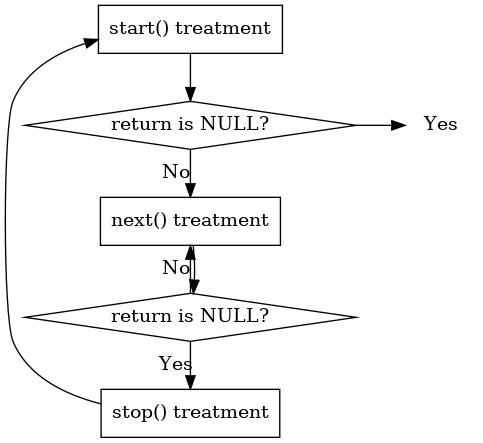
\includegraphics[width=.9\linewidth]{img/seq_file.png}

Seq\_file fournit des fonctions basiques pour la structure file\_operations, telles que seq\_read, seq\_lseek ou d'autres. Mais aucune fonction n'est fournit pour écrire dans notre fichier. Vous pouvez bien sûr utiliser les mêmes méthodes que dans notre exemple précédent pour le faire.

\begin{verbatim}
/**
 *  procfs4.c -  Cree un "fichier" dans /proc
 *      Ce programme utilise la bibliothèque seq_file pour gérer
 *      le fichier /proc
 */

#include <linux/kernel.h>
#include <linux/module.h>
#include <linux/proc_fs.h>      /* Nécessaire pour utiliser le proc fs */
#include <linux/seq_file.h>     /* Nécessaire pour seq_file */

#define PROC_NAME       "iter"

MODULE_AUTHOR("Philippe Reynes");
MODULE_LICENSE("GPL");

/**
 * Cette fonction est appelée au début d'une séquence, par exemple quand :
 *      - Le fichier /proc est lu (pout la première fois)
 *      - A la fin de la la fonction stop (fin de séquence)
 */
static void *my_seq_start(struct seq_file *s, loff_t *pos)
{
    static unsigned long counter = 0;

    /* Est-ce qu'on commande une nouvelle séquence ? */
    if ( *pos == 0 ) {
        /* Si oui => Renvoie une valeur non nulle pour démarrer la séquence */
        return &counter;
    }
    else {
        /*
         * Sinon => Signifie la fin de la séquence, renvoie NULL pour
         * arrêter la lecture
         */
        *pos = 0;
        return NULL;
    }
}

/**
 * Cette fonction est appelée après le début la séquence.
 * Elle est appelée en boucle jusqu'à ce qu'elle renvoie la valeur NULL.
 * Cette valeur signifie la fin de la séquence.
 */
static void *my_seq_next(struct seq_file *s, void *v, loff_t *pos)
{
    unsigned long *tmp_v = (unsigned long *)v;
    (*tmp_v)++;
    (*pos)++;
    return NULL;
}

/**
 * Cette fonction est appelée à la fin de la séquence.
 */
static void my_seq_stop(struct seq_file *s, void *v)
{
    /*
     * Rien à faire, on utilise une variable
     * statique dans la fonction start()
     */
}

/*
 * Cette fonction est appelée à chaque étape d'une séquence.
 */
static int my_seq_show(struct seq_file *s, void *v)
{
    loff_t *spos = (loff_t *) v;

    seq_printf(s, "%Ld\n", *spos);
    return 0;
}

/*
 * Cette structure définit les fonctions qui gèreront la séquence
 */
static struct seq_operations my_seq_ops = {
        .start = my_seq_start,
        .next  = my_seq_next,
        .stop  = my_seq_stop,
        .show  = my_seq_show
};

/*
 * Cette fonction est appelée quand le fichier /proc sera ouvert
 */
static int my_open(struct inode *inode, struct file *file)
{
    return seq_open(file, &my_seq_ops);
};

/*
 * Cette structure définit les fonctions qui géreront le fichier /proc
 */
static struct file_operations my_file_ops = {
    .owner   = THIS_MODULE,
    .open    = my_open,
    .read    = seq_read,
    .llseek  = seq_lseek,
    .release = seq_release
};


/*
 * Cette fonction sera appelée quand le module sera chargé
 */
int init_module(void)
{
    struct proc_dir_entry *entry;

    entry = proc_create(PROC_NAME, 0, NULL, &my_file_ops);
    if(entry == NULL)
    {
        remove_proc_entry(PROC_NAME, NULL);
        pr_debug("Error: Could not initialize /proc/%s\n", PROC_NAME);
        return -ENOMEM;
    }

    return 0;
}

/*
 * Cette fonction sera appelée quand le module sera déchargé du noyau
 */
void cleanup_module(void)
{
    remove_proc_entry(PROC_NAME, NULL);
    pr_debug("/proc/%s supprime\n", PROC_NAME);
}
\end{verbatim}

Si vous désirez plus d'informations, je vous conseille ce lien :

\begin{itemize}
\item \url{http://lwn.net/Articles/22355/}

\item \url{http://www.kernelnewbies.org/documents/seq_file_howto.txt}
\end{itemize}

Vous pouvez également lire le code de fs/seq\_file.c au sein du noyau.

\section*{sysfs : Interagissez avec votre module}
\label{sec-8}

\emph{sysfs} vous permet d'interagir avec le noyau depuis l'espace utilisateur, via la lecture ou l'écriture de variable au sein de modules. Ça peut être très utile à des fins de débogage, ou encore cela peut vous servir d'interface pour vos applications ou vos scripts. Vous pouvez trouvez des répertoires et des fichiers sysfs au sein du répertoire \emph{sys} de votre système.

\begin{verbatim}
ls -l /sys
\end{verbatim}

L'éternel exemple du module hello world incluant la création d'une variable accessible via sysfs est fourni plus bas :

\begin{verbatim}
/*
 * hello-sysfs.c sysfs example
 */

#include <linux/module.h>
#include <linux/kobject.h>
#include <linux/sysfs.h>
#include <linux/init.h>
#include <linux/fs.h>
#include <linux/string.h>

MODULE_LICENSE("GPL");
MODULE_AUTHOR("Bob Mottram");

static struct kobject *mymodule;

/* La variable que vous souhaitez pouvoir modifier */
static int myvariable = 0;

static ssize_t myvariable_show(struct kobject *kobj,
                               struct kobj_attribute *attr,
                               char *buf)
{
    return sprintf(buf, "%d\n", myvariable);
}

static ssize_t myvariable_store(struct kobject *kobj,
                                struct kobj_attribute *attr,
                                char *buf, size_t count)
{
    sscanf(buf, "%du", &myvariable);
    return count;
}


static struct kobj_attribute myvariable_attribute =
    __ATTR(myvariable, 0660, myvariable_show,
           (void*)myvariable_store);

static int __init mymodule_init (void)
{
    int error = 0;

    pr_info("mymodule: initialised\n");

    mymodule =
        kobject_create_and_add("mymodule", kernel_kobj);
    if (!mymodule)
        return -ENOMEM;

    error = sysfs_create_file(mymodule, &myvariable_attribute.attr);
    if (error) {
        pr_info("failed to create the myvariable file " \
               "in /sys/kernel/mymodule\n");
    }

    return error;
}

static void __exit mymodule_exit (void)
{
    pr_info("mymodule: Exit success\n");
    kobject_put(mymodule);
}

module_init(mymodule_init);
module_exit(mymodule_exit);
\end{verbatim}

Créez et installez votre module :

\begin{verbatim}
make
sudo insmod hello-sysfs.ko
\end{verbatim}

Vérifiez qu'il existe :

\begin{verbatim}
sudo lsmod | grep hello_sysfs
\end{verbatim}

Quelle est la valeur de \emph{myvariable} ?

\begin{verbatim}
cat /sys/kernel/mymodule/myvariable
\end{verbatim}

Modifiez la valeur de \emph{myvariable} et vérifiez qu'elle a changée

\begin{verbatim}
echo "32" > /sys/kernel/mymodule/myvariable
cat /sys/kernel/mymodule/myvariable
\end{verbatim}

Finalement, supprimez ce module exemple :

\begin{verbatim}
sudo rmmod hello_sysfs
\end{verbatim}

\section*{Interagir avec un fichier de périphérique}
\label{sec-9}

Les fichiers de périphériques sont censés représenter des périphériques physiques. La plupart de ces périphériques physiques sont utilisés aussi bien en lecture qu'en écriture, il existe donc des mécanismes pour que le pilote du périphérique concerné reçoive des informations du processus qui souhaite écrire dans le périphérique. Ce mécanisme est réalisé en ouvrant le fichier du périphérique pour une écriture, et en écrivant dedans, tout comme vous écririez dans un simple fichier. Dans l'illustration suivante, un exemple vous est donné via la fonction device\_write.

Mais ce n'est pas suffisant. Imaginez que vous disposez d'un port série, lequel est connecté à une carte réseau (même si vous avez une carte réseau intégrée dans votre carte mère, celle-ci est implantée, du point de vue du processeur, comme un port série connecté à une carte réseau, vous n'aurez donc pas à pousser loin votre imagination). Le comportement qui pourra vous sembler naturel sera d'utiliser le fichier de périphérique du port série vers la carte réseau pour y écrire (soit des ordres pour commander la carte réseau, soit des données à transmettre sur la ligne) ou pour y lire des informations depuis la carte réseau (soit les réponses des commandes, soit des données reçues depuis la ligne). Vous avez réglé le problème, mais la question reste ouverte de savoir comment vous ferez quand vous souhaiterez interagir avec le port-série lui-même, par exemple pour définir à quelle fréquence il doit recevoir et envoyer des données.

La réponse au sein d'Unix est d'utiliser une fonction spéciale appelée \textbf{ioctl} (raccourci pour Input Output ConTrol). Chaque périphérique a ses propres commandes ioctl, qui peuvent être soit en lecture (envoyer des informations du processus vers le noyau), soit en écriture (renvoyer les informations Au processus), soit les deux, soit aucune des deux. Vous noterez qu'ici, les rôles des fonctions de lecture et d'écritures sont inversées une fois de plus. Ainsi avec les ioctl, la lecture consiste à envoyer des informations vers le noyau, et l'écriture consiste à recevoir des informations du noyau.

Les fonctions ioctl sont appelées avec trois paramètres : le file descriptor du fichier de périphérique approprié, le numéro d'ioctl, et un paramètre de type long afin que vous puissiez le caster pour passer l'adresse de tout ce que vous souhaitez.

Le numéro de l'ioctl est une valeur formatée qui contient le numéro majeur de votre périphérique, le type de l'ioctl, la commande, et le type de votre paramètre. Le numéro d'ioctl est habituellement créé dans une fichier d'en-tête via un appel de macro ($\backslash$\_IO, $\backslash$\_IOR, $\backslash$\_IOW ou $\backslash$\_IOWR , en fonction du type). Ce fichier d'entête devra ensuite également être inclus à la fois par le programme utilisateur qui va employer l'ioctl (afin qu'il puisse générer un numéro correct), et par le module (afin qu'il puisse comprendre ce numéro). Dans l'exemple suivant, le fichier d'en-tête est chardev.h et le programme utilisateur qui exécute l'ioctl est ioctl.c

Si vous souhaitez utiliser les ioctls pour votre propre module, la meilleure manière est de demander un numéro officiel, ainsi vous ne risquez pas de partager votre numéro avec un autre, dans quel cas le résultat pourrait être désastreux. Pour plus d'informations, jetez un oeil au fichier Documentation/ioctl-number.txt au sein des sources de votre noyau.

\begin{verbatim}
/*
 * chardev2.c - Créé un périphérique d'entrée/sortie en mode caractère
 */

#include <linux/kernel.h>
#include <linux/module.h>
#include <linux/fs.h>
#include <linux/init.h>
#include <linux/delay.h>
#include <linux/device.h>
#include <linux/irq.h>
#include <asm/uaccess.h>
#include <asm/irq.h>
#include <asm/io.h>
#include <linux/poll.h>
#include <linux/cdev.h>

#include "chardev.h"
#define SUCCESS 0
#define DEVICE_NAME "char_dev"
#define BUF_LEN 80

/*
 * Est-ce que le périphérique est
 * actuellement ouvert ?
 * Utilisé pour éviter les accès
 * concurrents au même périphériques
 */
static int Device_Open = 0;

/*
 * Le message que fournira le périphérique quand on lui demandera
 */
static char Message[BUF_LEN];

/*
 * Où en est le processus qui lit le message ?
 * Utile si message est plus grand que la taille du tampon à remplir dans
 * la fonction device_read()
 */
static char *Message_Ptr;

static int Major; /* Numéro Major associé au pilote de notre périphérique */
static struct class *cls;

/*
 * C'est appelé quand un processus demande une ouverture du fichier associé
 * à notre périphérique
 */
static int device_open(struct inode *inode, struct file *file)
{
#ifdef DEBUG
        pr_info("device_open(%p)\n", file);
#endif

    /*
     * On ne souhaite pas traiter deux processus concurentiellement
     */
    if (Device_Open)
        return -EBUSY;

    Device_Open++;
    /*
     * Initialise le message
     */
    Message_Ptr = Message;
    try_module_get(THIS_MODULE);
    return SUCCESS;
}

static int device_release(struct inode *inode, struct file *file)
{
#ifdef DEBUG
    pr_info("device_release(%p,%p)\n", inode, file);
#endif

    /*
     * Nous sommes maintenant prêt pour traiter l'appel suivant
     */
    Device_Open--;

    module_put(THIS_MODULE);
    return SUCCESS;
}

/*
 * Cette fonction est appelée quand un processus qui a déjà ouvert le fichier
 * associé à notre périphérique demande une lecture de ce dernier
 */
static ssize_t device_read(struct file *file,   /* voir include/linux/fs.h  */
                           char __user * buffer,        /* Tampon qui sera  *
                                                         * remplis          */
                           size_t length,       /* Taille du tampon         */
                           loff_t * offset)
{
    /*
     * Nombre d'octets réellement écrits dans le tampon
     */
    int bytes_read = 0;

#ifdef DEBUG
    pr_info("device_read(%p,%p,%d)\n", file, buffer, length);
#endif

    /*
     * Si on atteint la fin du message, renvoie un 0 pour signifier
     * la fin du fichier
     */
    if (*Message_Ptr == 0)
        return 0;

    /*
     * Insertion des données dans le tampon
     */
    while (length && *Message_Ptr) {
    /*
     * Parce que le tampon est dans l'espace utilisateur, et non pas dans
     * l'espace noyau où nous nous trouvons au moment où l'on exécute ce
     * code, une simple modification de valeur par les variable ne
     * fonctionnerait pas. C'est pourquoi nous devons utiliser la fonction
     * put_user() qui copie des données de l'espace noyau vers l'espace
     * utilisateur
     */
     put_user(*(Message_Ptr++), buffer++);
     length--;
     bytes_read++;
}

#ifdef DEBUG
    pr_info("Read %d bytes, %d left\n", bytes_read, length);
#endif
    /*
     * La plupart des fonctions de lecture renvoie le nombre d'octets
     * qui ont été inséré dans le tampon
     */
    return bytes_read;
}

/*
 * Cette fonction sera appelée quand quelqu'un commandera une écriture
 * dans le fichier associé à notre périphérique
 */
static ssize_t
device_write(struct file *file,
             const char __user * buffer, size_t length, loff_t * offset)
{
    int i;

#ifdef DEBUG
    pr_info("device_write(%p,%s,%d)", file, buffer, length);
#endif

    for (i = 0; i < length && i < BUF_LEN; i++)
        get_user(Message[i], buffer + i);

    Message_Ptr = Message;

    /*
     * Une fois n'est pas coutume, nous renvoyons
     * le nombre de caractères traités
     */
    return i;
}

/*
 * Cette fonction sera appelée quand un processus essaiera de commander
 * un ioctl sur le fichier associé à notre périphérique. Par rapport aux
 * structures inode et file, on a ici deux paramètres supplémentaires :
 * le numéro de l'ioctl appelé et le paramètre passé à la fonction ioctl.
 *
 * Si l'ioctl est en mode écriture, ou lecture/écriture, ce qui implique
 * qu'une valeur sera renvoyée au processus l'exécutant, alors l'appel
 * ioctl renverra la même chose que cette fonction.
 */
long device_ioctl(struct file *file,
                  unsigned int ioctl_num,    /* Numéro de l'appel ioctl    */
                  unsigned long ioctl_param) /* Paramètre de l'appel ioctl */
{
    int i;
    char *temp;
    char ch;

    /*
     * Switch en fonction du numéro de l'appel ioctl
     */
    switch (ioctl_num) {
    case IOCTL_SET_MSG:
        /*
         * Reçoit via le paramètre de l'appel ioctl
         * un pointeur vers un message (dans l'espace utilisateur)
         * et le modifie pour qu'il pointe vers le message de notre
         * périphérique.
         */
        temp = (char *)ioctl_param;

         /*
          * Cherche la taille de notre message
          */
         get_user(ch, temp);
         for (i = 0; ch && i < BUF_LEN; i++, temp++)
             get_user(ch, temp);

         device_write(file, (char *)ioctl_param, i, 0);
         break;

    case IOCTL_GET_MSG:
        /*
         * Renvoie un message au processus qui demande une lecture
         * Notre paramètre est un pointeur, il faut donc le remplir
         */
        i = device_read(file, (char *)ioctl_param, 99, 0);

        /*
         * Puis pour faire faire les choses proprement,
         * il faut insérer un 0 à la fin du tampon
         */
        put_user('\0', (char *)ioctl_param + i);
        break;

    case IOCTL_GET_NTH_BYTE:
        /*
         * Cette ioctl est à la fois en mode entrée (ioctl_param)
         * et en mode sortie (la valeur renvoyée par cette fonction)
         */
        return Message[ioctl_param];
        break;
    }

    return SUCCESS;
}

/* Déclarations des module */

/*
 * Cette structure va contenir les fonctions qui seront appelées au moment
 * où un processus agira sur le périphérique qu'on a créé. Comme un pointeur
 * vers cette structure est conservé dans la table des périphériques, ce
 * dernier ne peut pas être local à init_module.
 *
 * La valeur NULL est assignée aux fonctions non implantées.
 */
struct file_operations Fops = {
        .read = device_read,
        .write = device_write,
        .unlocked_ioctl = device_ioctl,
        .open = device_open,
        .release = device_release,     /* Fonction de fermeture */
};

/*
 * Initialiser le module - Enregistrer le périphérique de type caractère
 */
int init_module()
{
    int ret_val;
    /*
     * Enregistre le périphérique de type caractère
     * (ou du moins essaie de le faire)
     */
    ret_val = register_chrdev(MAJOR_NUM, DEVICE_NAME, &Fops);

    /*
     * Les valeurs négatices signifient des erreurs
     */
    if (ret_val < 0) {
        pr_alert("%s failed with %d\n",
                 "Sorry, registering the character device ", ret_val);
        return ret_val;
    }

    Major = ret_val;

    cls = class_create(THIS_MODULE, DEVICE_FILE_NAME);
    device_create(cls, NULL, MKDEV(Major, MAJOR_NUM), NULL, DEVICE_FILE_NAME);

    pr_info("Device created on /dev/%s\n", DEVICE_FILE_NAME);

    return 0;
}

/*
 * Nettoyage - Supprime le fichier approprié de /proc
 */
void cleanup_module()
{
    device_destroy(cls, MKDEV(Major, 0));
    class_destroy(cls);

    /*
     * Supprime le périphérique
     */
    unregister_chrdev(Major, DEVICE_NAME);
}
\end{verbatim}

\begin{verbatim}
/*
 *  chardev.h - Le fichier d'en-tête qui contient toutes les définitions
 *  d'ioctl
 *
 *  Les déclarations ici doivent obligatoirement être contenues dans ce type
 *  de fichier, parce qu'elles doivent être connues à la fois :
 *  - de notre module (dans le fichier chardev.c)
 *  - et par le processus qui appelle les ioctl (ioctl.c).
 */

#ifndef CHARDEV_H
#define CHARDEV_H

#include <linux/ioctl.h>

/*
 * Le numéro majeur de périphérique.
 * On ne peut plus utiliser un mécanisme d'attribution dynamique, car les
 * ioctls doivent le connaître.
 */
#define MAJOR_NUM 100

/*
 * Assigne le message du pilote de notre périphérique
 * depuis un processus utilisateur
 */
#define IOCTL_SET_MSG _IOW(MAJOR_NUM, 0, char *)
/*
 * _IOW signifie qu'on est en train de créer un numéro d'ioctl
 * pour passer des informations depuis un processus utilisateur
 * vers un module noyau.
 *
 * Le premier argument, MAJOR_NUM, est le numéro majeur du périphérique
 * qu'on utilise.
 *
 * Le deuxième argument est le numéro de la commande.
 * Au sein d'un pilote, il peut exister différentes commandes ioctl. Ce numéro
 * sert à les identifier
 *
 * Le troisième argument est le type qu'on attend du processus exécutant
 * une commande ioctl.
 */

/*
 * Obtiens le message du pilote de notre périphérique
 */
#define IOCTL_GET_MSG _IOR(MAJOR_NUM, 1, char *)
/*
 * Cet IOCTL est utilisé pour diffuser une information, pour informer le
 * processus du contenu de notre pilote. Cependant, on a encore besoin
 * d'un tampon pour y insérer les données que l'utilisateur souhaite,
 * tampon qui nous est fourni par ce dernier.
 */

/*
 * Obtenir le Nème caractère de notre message
 */
#define IOCTL_GET_NTH_BYTE _IOWR(MAJOR_NUM, 2, int)
/*
 * L'IOCTL est utilisé à la fois en sortie et en entrée.
 * Il reçoit un numéro N de l'utilisateur, et renvoie Message[N]
 */

/*
 * Le nom du fichier associé à notre périphérique
 */
#define DEVICE_FILE_NAME "char_dev"

#endif
\end{verbatim}

\begin{verbatim}
/*
 *  ioctl.c - Le programme utilisateur qui exécutera des ioctls pour
 *  intéragir avec notre module
 *
 *  Jusqu'Ã  maintenant, nous pouvions utiliser des commandes comme cat
 *  pour commander une entrée ou une sortie sur nos modules, mais
 *  pour exécuter un appel ioctl, il faut nécessairement écrire notre
 *  propre programme utilisateur
 */

/*
 * Spécifique à notre périphérique, ce fichier contient les numéro des ioctls
 * et le numéro majeur du fichier associé à notre périphérique.
 */
#include "../chardev.h"

#include <stdio.h>
#include <stdlib.h>
#include <fcntl.h>     /* open */
#include <unistd.h>    /* exit */
#include <sys/ioctl.h> /* ioctl */

/*
 * Fonction pour les appels ioctls
 */

int ioctl_set_msg(int file_desc, char *message)
{
    int ret_val;

    ret_val = ioctl(file_desc, IOCTL_SET_MSG, message);

    if (ret_val < 0) {
        printf("ioctl_set_msg failed:%d\n", ret_val);
        exit(-1);
    }
    return 0;
}

int ioctl_get_msg(int file_desc)
{
    int ret_val;
    char message[100];

    /*
     * Attention ! Ceci est dangereux parce qu'on ne dit pas au noyau
     * jusqu'où il doit écrire, alors il existe un risque de dépassement
     * du tampon. En condition réelle de programmation noyau, nous
     * aurions utilisé deux appels ioctls :
     * - un pour informer le noyau de la taille du tampon
     * - un second avec le tampon à remplir
     */
    ret_val = ioctl(file_desc, IOCTL_GET_MSG, message);

    if (ret_val < 0) {
        printf("ioctl_get_msg failed:%d\n", ret_val);
        exit(-1);
    }

    printf("get_msg message:%s\n", message);
    return 0;
}

int ioctl_get_nth_byte(int file_desc)
{
    int i;
    char c;

    printf("get_nth_byte message:");

    i = 0;
    do {
        c = ioctl(file_desc, IOCTL_GET_NTH_BYTE, i++);

        if (c < 0) {
            printf("ioctl_get_nth_byte failed at the %d'th byte:\n",
                   i);
            exit(-1);
        }

        putchar(c);
    } while (c != 0);
    putchar('\n');
    return 0;
}

/*
 * Main - Appel des fonctions d'ioctls
 */
int main()
{
    int file_desc, ret_val;
    char *msg = "Message passed by ioctl\n";

    file_desc = open(DEVICE_FILE_NAME, 0);
    if (file_desc < 0) {
        printf("Can't open device file: %s\n", DEVICE_FILE_NAME);
        exit(-1);
    }

    ioctl_get_nth_byte(file_desc);
    ioctl_get_msg(file_desc);
    ioctl_set_msg(file_desc, msg);

    close(file_desc);
    return 0;
}
\end{verbatim}

\section*{Les appels système}
\label{sec-10}

Jusqu'ici, tout ce qu'on a fait était d'utiliser des mécanismes prédéfinis pour enregistrer un fichier \textbf{/proc} et des gestionnaires de périphériques. Ça vous suffira tant que vous vous cantonnez à ce que les développeurs noyaux ont prévu pour vous, comme écrire un pilote de périphérique. Mais qu'en est-il si vous souhaitez aller plus loin ? Si vous souhaitez modifier le fonctionnement du système ?

Si vous n'avez pas encore succombé aux sirènes de la machine virtuelle, alors c'est ici que le développement du noyau peut vraiment devenir dangereux. Pendant que j'ai écrit l'exemple plus bas, J'ai tué l'appel système \textbf{open()}. Ce qui signifie que : je ne pouvais plus ouvrir aucun fichier, je ne pouvais plus lancer aucun programme, et je ne pouvais plus éteindre le système. J'ai dû redémarrer brutalement ma machine virtuelle. Je n'ai perdu aucun fichier important, mais si j'avais fait de même sur une vraie machine, ce cauchemar aurait pu devenir réalité. Pour vous assurer de ne pas perdre de fichier, même au sein d'un environnement d'essai, pensez à exécuter \textbf{sync} juste avant d'appeler \textbf{insmod} et \textbf{rmmod}.

Oubliez tout à propos des fichiers \textbf{/proc} et des fichiers de périphériques. Ce ne sont que des détails sans importance à l'échelle de votre système. Les vrais mécanismes de communication du noyau sont les appels système. Ce sont eux qui sont appelés par tous les processus. Quand un processus demande un service au noyau (tel qu'ouvrir un fichier, créer un nouveau processus, ou demander plus de mémoire), c'est ce mécanisme qui est appelé. Si vous souhaitez changer le fonctionnement de votre noyau, c'est par là que vous devrez passer. Comme j'en ai parlé plus tôt, si vous souhaitez voir tous les appels système effectués par un programme, utilisez la commande \textbf{strace}.

En général, un processus n'est pas censé pouvoir accéder au noyau. Il ne peut ni accéder à la mémoire du noyau, ni appeler les fonctions du noyau. Le matériel, via le CPU, s'en assure (c'est la raison pour laquelle ce mécanisme est appelé 'mode superviseur', ou 'protection de pages').

Les appels système sont une exception à cette règle générale. Ce qui se passe, c'est que les processus remplissent des registres avec des valeurs en guise de paramètres, et appellent ensuite une instruction particulière qui saute à une adresse définie précédemment, au sein du noyau (bien sûr, cette adresse peut être lue par les processus utilisateurs, mais ces derniers ne peuvent pas y écrire). Au sein des CPU Intels, on y accède via l'interruption 0x80. Le matériel sait qu'une fois que vous avez sauté à cette adresse, votre processeur n'est plus en mode utilisateur, mais en mode noyau --- vous êtes donc libre de faire tout ce que vous souhaitez.

L'adresse au sein du noyau où un processus peut sauter est appelé system\_call. L'algorithme à l'arrivée de ce code regarde le numéro d'appel système, qui définit quelle fonction système est demandée. Ensuite, le programme regarde dans la table d'appels système (appelée sys\_call\_table) quelle est l'adresse de la fonction demandée. Pour finir, le processeur saute à cette fonction, et avant d'en revenir, effectue quelques vérifications systèmes avant de redonner la main au processus utilisateur appelant (ou à un autre processus si le premier à été trop long). Si vous souhaitez lire ce code, il est disponible dans le code source (arch/\$<\$architecture\$>\$/kernel/enty.S, après la ligne ENTRY(system\_call)).

Ainsi, si vous souhaitez, d'une certaine manière, changer le fonctionnement d'un certain appel système, ce que vous devez faire est de créer votre propre fonction pour l'insérer (généralement cette fonction exécutera votre code avant d'appeler la fonction système originale) et ensuite changer le pointeur de la table sys\_call\_table pour que cette dernière pointe vers votre fonction. Attention ! Parce que vous ne souhaitez pas que votre module soit enlevé en laissant le système dans un état instable, il est important que la fonction cleanup\_module modifie la table dans son état précédent.

Le code source suivant est un exemple d'un tel module noyau. On souhaite ici "espionner" un certain utilisateur, afin de notifier, via \textbf{pr\_info()}, quand cet utilisateur ouvre un fichier. Pour procéder, on remplace l'appel système lancé à l'ouverture d'un fichier par notre propre fonction, appelée ici \textbf{our\_sys\_open}. Cette fonction vérifie l'uid (l'identifiant de l'utilisateur) du processus courant, et si cet uid est égal à celui qu'on surveille, alors la fonction appelle \textbf{pr\_info()} afin d'afficher le nom du fichier en cours d'ouverture. Ensuite, et peu importe l'uid, notre fonction appelle la fonction originale open() avec les mêmes paramètres, pour effectivement ouvrir le fichier.

La fonction \textbf{init\_module} remplace la fonction concernée dans la table \textbf{sys\_call\_table} avec notre fonction, et conserve l'originale dans une variable. La fonction cleanup\_module utilise cette variable pour restaurer le système dans l'état où il se trouvait avant cette modification. Cette méthode est très dangereuse, dans le cas ou deux modules noyaux modifient le même appel système.

Imaginez deux modules, A et B. L'ouverture de A sera A\_open, et celle de B B\_open. Maintenant, quand A est inséré dans le noyau, l'appel système open est remplacé par A\_open, qui appellera l'appel original open à sa fin. Ensuite, si on insère B au sein de noyau, ce dernier remplacera l'appel système A\_open avec le B\_open. L'appel de A\_open sera sonc effectué à la fin de la fonction B\_open.

Ensuite, enlevons ces modules. Si B est enlevé en premier, alors il n'y aura aucun problème --- l'appel système sera restauré à A\_open, qui lui-même appelle l'open() original. Cependant, si A est enlevé, alors l'appel système original sera restauré (ce qui signifie que B\_open ne sera jamais appelé). C'est problématique, mais pas catastrophique. Cependant, si vous enlevez ensuite B, la suppression de ce dernier va restaurer l'appel système à ce qu'il pense être l'original, \textbf{A\_open}, lequel n'est plus présent en mémoire. Les conséquences seront désastreuses.

À première vue, un module peut régler ce problème en vérifiant, lors de sa suppression, si l'appel système présent dans la table sys\_call\_table est bien sa propre fonction, et si ce n'est pas le cas, il ne doit rien changer (ainsi B ne changerait aucun appel système à sa suppression), mais cette solution conduirait en réalité à un problème plus grave encore. Quand A est enlevé, ce dernier voit que l'appel système a été changé à \textbf{B\_open}. Ce dernier ne restaurera donc pas l'appel système original. Mais malheureusement, B n'a pas conscience de ça. \textbf{B\_open} commencera, puis appellera \textbf{A\_open}, qui n'existe pas en mémoire. Donc même sans enlever B du système, votre système va planter.

Notez que tous les problèmes relatifs à cette situation rendent tout simplement la redéfinition des appels système impossible pour des usages en situation de production. Afin de ne pas tenter les développeurs du dimanche de faire des choses potentiellement désastreuses, la table \textbf{sys\_call\_table} n'est plus exportée, ce qui signifie que si vous souhaitez exécuter l'exemple suivant, vous devrez modifier votre noyau pour exporter la table en question. Dans le répertoire examples, vous trouverez un README et la modification à apporter. Comme vous l'imaginez, une telle modification ne doit pas être prise à la légère. N'essayez pas de réaliser une telle action sur un système important (par exemple un système que vous ne possédez pas ou que vous ne pouvez pas restaurer aisément). Vous aurez besoin d'accéder au code source complet de ce guide pour avoir accès aux modifications et au README. En fonction de votre version du noyau, vous risquez même devoir effectuer cette modification à la main.

C'est ici que se clôt ce chapitre. Sachez cependant que si Le Coyote chassant Bip Bip était un hacker noyau, ce serait la première chose qu'il essaierait pour attraper son repas !

\begin{verbatim}
/*
 *  syscall.c
 *
 *  Exemple de "vol" d'un d'appel système.
 *
 *  Désactive la protection des pages au niveau du processeur
 *  en changeant le 16ème bit dans le registre cr0
 *  (spécifique aux processeurs Intel)
 *
 *  Démonstration basée sur l'exemple de Peter Jay Salzman et sur
 *  https://bbs.archlinux.org/viewtopic.php?id=139406
 */

#include <linux/module.h>
#include <linux/kernel.h>
#include <linux/syscalls.h>
#include <linux/delay.h>
#include <asm/paravirt.h>
#include <linux/moduleparam.h>  /* Qui contiendra les paramètres */
#include <linux/unistd.h>       /* La liste des appels système */

/*
 * On a besoin de ces fichiers afin de connaître qui est
 * l'utilisateur dans la structure du processus actuel
 */
#include <linux/sched.h>
#include <linux/uaccess.h>

unsigned long **sys_call_table;
unsigned long original_cr0;

/*
 * UID qu'on souhaite espionner - sera affectée
 * par la ligne de commande
 */
static int uid;
module_param(uid, int, 0644);

/*
 * La prochaine variable est un pointeur qui contiendra l'adresse
 * de l'appel système avant notre modification.
 *
 * On garde cette adresse dans ce pointeur pour pouvoir, quand on déchargera
 * notre module, remettre le système dans son état initial. On doit garder en
 * mémoire dans ce pointeur l'appel système avant qu'on le modifie, et on ne
 * peut pas juste utiliser l'appel système original (sys_open) dans le cas ou
 * un autre module a modifié cet appel système avant non. Notez bien que cette
 * sécurité n'est pas absolument sûre, car dans le cas redouté décrit dans
 * ce guide de deux modules modifiant le même appel système, alors si le
 * module qui a modifié l'appel système original est supprimé avant le notre,
 * alors si j'appelle une fonction de ce module supprimé dépuis, je ne sais
 * pas ce qui attends notre noyau !
 *
 * Une autre raison pour laquelle on utilise ce pointeur c'est que sys_open
 * est une variable statique, et elle n'est donc pas exportée.
 */
asmlinkage int (*original_call) (const char *, int, int);

/*
 * La fonction suivante va remplacer sys_open
 * Elle sera donc appelée quand n'importe quel processus exécutera l'appel
 * système open.
 * Pour trouver le prototype exact, afin que correspondent parfaitement
 * les arguments, vous devrez faire un tour dans le fichier qui contient la
 * fonction originale (fs/open.c).
 *
 * En théorie, ça veut dire que notre code est donc dépendant de la version
 * actuelle du noyau, puisque notre fonction dépend des types et nombres
 * d'arguments que prennent l'appel système original.
 * En pratique, ne vous inquiétez pas, les appels système ne sont quasiment
 * jamais modifiés (cela signifirai que tous les programmes conçus avant cette
 * mise à jour soit recompilés, puisque les appels système sont l'interface
 * entre le noyau et les processus, et ça causerait donc des ravages
 * dévastateurs pour le noyau et sa réputation)
 */
asmlinkage int our_sys_open(const char *filename, int flags, int mode)
{
    int i = 0;
    char ch;

    /*
     * Note l'ouverture du fichier, si nécessaire
     */
    pr_info("Opened file by %d: ", uid);
    do {
        get_user(ch, filename + i);
        i++;
        pr_info("%c", ch);
    } while (ch != 0);
    pr_info("\n");

    /*
     * A là fin de notre appel système, notre code doit, bien sur, appeler
     * le code original, sinon quoi on perdrait la capacité d'ouvrir
     * tous les fichiers
     */
    return original_call(filename, flags, mode);
}

static unsigned long **aquire_sys_call_table(void)
{
    unsigned long int offset = PAGE_OFFSET;
    unsigned long **sct;

    while (offset < ULLONG_MAX) {
        sct = (unsigned long **)offset;

        if (sct[__NR_close] == (unsigned long *) sys_close)
            return sct;

        offset += sizeof(void *);
    }

    return NULL;
}

static int __init syscall_start(void)
{
    if(!(sys_call_table = aquire_sys_call_table()))
        return -1;

    original_cr0 = read_cr0();

    write_cr0(original_cr0 & ~0x00010000);

    /* Garde l'adresse de l'appel système open original */
    original_call = (void*)sys_call_table[__NR_open];

    /* Modifie la table des appels système pour utiliser notre fonction */
    sys_call_table[__NR_open] = (unsigned long *)our_sys_open;

    write_cr0(original_cr0);

    pr_info("Spying on UID:%d\n", uid);

    return 0;
}

static void __exit syscall_end(void)
{
    if(!sys_call_table) {
        return;
    }

    /*
     * Restaure la table des appels système Ã
     * son état avant notre modification
     */
    if (sys_call_table[__NR_open] != (unsigned long *)our_sys_open) {
        pr_alert("Somebody else also played with the ");
        pr_alert("open system call\n");
        pr_alert("The system may be left in ");
        pr_alert("an unstable state.\n");
    }

    write_cr0(original_cr0 & ~0x00010000);
    sys_call_table[__NR_open] = (unsigned long *)original_call;
    write_cr0(original_cr0);

    msleep(2000);
}

module_init(syscall_start);
module_exit(syscall_end);

MODULE_LICENSE("GPL");
\end{verbatim}

\section*{Processus bloquants et threads}
\label{sec-11}
\subsection*{Sleep}
\label{sec-11-1}
Que faites-vous quand quelqu'un vous demande de faire quelque chose que vous ne pouvez pas faire immédiatement ? Si vous êtes un Corse dérangé par quelqu'un vous lui répondrez sans doute "\emph{Pas maintenant, laisse-moi dormir !}". Mais si vous êtes un module et que vous êtes dérangé par un processus, vous avez une autre possibilité : Vous pouvez endormir le processus qui vous demande jusqu'à ce que vous puissiez vous en occuper. Après tout, les processus sont endormis et réveillés sans arrêt par le noyau (c'est la raison pour laquelle de nombreux processus donnent l'impression de tourner en même temps sur un seul processeur).

Le module noyau suivant est un exemple de ça. Le fichier (appelé \textbf{/proc/sleep}) ne peut être ouvert que par un seul processus à la fois. Si le fichier est déjà ouvert, le module appelle wait\_event\_interruptible. La manière la plus simple de garder un fichier ouvert est la suivante :

\begin{verbatim}
tail -f
\end{verbatim}

La fonction wait\_event\_interruptible change l'état de la tâche (une tâche est ni plus ni moins qu'une structure de données dans le noyau qui contient les informations d'un processus et les appels système utilisés) pour \textbf{TASK\_INTERRUPTIBLE}, qui signifie que la tâche ne sera pas lancée avant qu'elle ne soit réveillée d'une quelconque manière. La fonction wait\_event\_interruptible va ensuite ajouter la tâche en question à WaitQ, la file des tâches qui attendent pour accéder au fichier. Ensuite, la fonction appelle l'ordonnanceur pour changer le contexte d'exécution de la thread à endormir pour une autre, qui sera vraiment utilisée par le CPU.

Quand le processus qui utilisait le fichier n'en a plus besoin, ce processus ferme le fichier, la fonction module\_close est alors appelée. Cette fonction réveille tous les processus dans la file d'attente (il n'y a pas de moyen de n'en réveiller qu'un). Quand cette fonction se termine, alors le processus qui vient de fermer le fichier peut continuer sa vie. En temps voulu, l'ordonnanceur décidera que ce processus a assez profité du processeur, et "donnera" le processeur à un autre processus. Et tôt ou tard, l'un des processus qui était dans la file d'attente pour le fichier se verra donner l'accès au processeur par l'ordonnanceur. Et il reprendra sa vie juste après l'appel à \textbf{module\_interruptible\_sleep\_on}.

Ça signifie que le processus est encore en train d'exécuter du code noyau. D'un point de vue du code utilisateur du programme, on est encore situé dans l'appel système open, lequel ne s'est pas encore terminé. Le processus n'a absolument aucune idée qu'un autre processus a utilisé le processeur entre le moment où il a exécuté l'appel à la fonction open() et le moment où cette fonction s'est terminée.

Une fois que le processus qui attendait l'accès au fichier a la main sur le processeur et sur le fichier, il peut ensuite affecter une variable globale pour signaler aux autres processus que le fichier est encore ouvert (en l'occurrence par lui), et continuer son affaire. Quand les autres processus qui attendent l'accès à ce fichier auront accès au processeur, ils liront que cette variable globale signale que le fichier sur lequel ils attendent un accès est encore occupé, et se rendormiront aussitôt.

Dans notre cas, nous utiliserons tail -f pour garder le fichier ouvert continuellement en tâche de fond, pendant que nous essaierons d'y accéder avec d'autres processus (toujours en tâche de fond, afin que nous n'ayons pas besoin de basculer vers un autre terminal). Dès que le premier fichier sera tué avec la commande kill\%1, alors le second se réveillera, aura finalement accès au fichier avant de se terminer.

Pour rendre cette expérience plus intéressante, sachez que bien que notre processus endormi attend son prince charmant, la fonction \textbf{module\_close} n'a pas le monopole du réveil de notre processus. Ce dernier peut être également réveillé par d'autre interruptions, telles qu'un signal Ctrl+c/ (\textbf{SIGINT}). Ceci vient du fait qu'on a préféré utiliser \textbf{module\_interruptible\_sleep\_on}. On aurait pu utiliser \textbf{module\_sleep\_on} à la place, lequel ignore les signaux, mais pour une raison qui m'échappe, les utilisateurs n'aiment pas avoir l'impression que le contrôle de leur machine leur échappe.

Dans le cas d'un réveil par Ctrl+c/, on veut terminer la fonction immédiatement et renvoyer un \textbf{-EINTR}. C'est essentiel afin que les utilisateurs puissent tuer un processus avant que ce dernier ne reçoivent le fichier qu'il attend.

Il y a encore un point important à retenir. Parfois, les processus sont exigeants et ne souhaitent pas s'endormir. Ils veulent soit obtenir ce qu'ils demandent immédiatement, soit qu'on leur informe que la ressource qu'ils demandent n'est pas disponible. De tels processus utilisent le drapeau \textbf{O\_NONBLOCK} quand ils ouvrent un fichier. Le noyau est censé intervenir en renvoyant une erreur \textbf{-EAGAIN} à l'appel d'une opération qui ignorerait ce drapeau pour bloquer le processus appelant. Le programme cat\_noblock, disponible dans le code source de ce chapitre de votre guide, peut être utiliser pour illustrer l'ouverture d'un fichier avec l'option \textbf{O\_NONBLOCK}.

\begin{verbatim}
hostname:~/lkmpg-examples/09-BlockingProcesses# insmod sleep.ko
hostname:~/lkmpg-examples/09-BlockingProcesses# cat_noblock /proc/sleep
Last input:
hostname:~/lkmpg-examples/09-BlockingProcesses# tail -f /proc/sleep &
Last input:
Last input:
Last input:
Last input:
Last input:
Last input:
Last input:
tail: /proc/sleep: file truncated
[1] 6540
hostname:~/lkmpg-examples/09-BlockingProcesses# cat_noblock /proc/sleep
Open would block
hostname:~/lkmpg-examples/09-BlockingProcesses# kill %1
[1]+  Terminated              tail -f /proc/sleep
hostname:~/lkmpg-examples/09-BlockingProcesses# cat_noblock /proc/sleep
Last input:
hostname:~/lkmpg-examples/09-BlockingProcesses#
\end{verbatim}

\begin{verbatim}
/*
 *  sleep.c - Créer un fichier /proc, et si
 *  plusieurs processus essaient d'y accèder
 *  en même temps, les endorts tous sauf un
 *  à qui la lecture est accordée
 */

#include <linux/kernel.h>
#include <linux/module.h>
#include <linux/proc_fs.h> /* Nécessaire comme nous utilisons proc fs */
#include <linux/sched.h>   /* Nécessaire pour endormir les processus  *
                              et les réveiller                        */
#include <linux/uaccess.h> /* Nécessaire pour les fonctions get_user  *
                              et put_user                             */

/*
 * Les fonctions de notre module
 */

/*
 * Dans ce tableau on garde le dernier message reçu,
 * afin de prouver que notre fichier gère les entrées
 */
#define MESSAGE_LENGTH 80
static char Message[MESSAGE_LENGTH];

static struct proc_dir_entry *Our_Proc_File;
#define PROC_ENTRY_FILENAME "sleep"

/*
 * Fonction de lecture associée dans notre struct file operations
 */
static ssize_t module_output(struct file *file, /* Voir include/linux/fs.h  */
                             char *buf,         /* Le tampon dans lequel on *
                                                   va insérer les données   *
                                                   (situé dans l'espace     *
                                                   utilisateur)             */
                             size_t len,        /* La taille du tampon      */
                             loff_t * offset)
{
    static int finished = 0;
    int i;
    char message[MESSAGE_LENGTH + 30];

    /*
     * Renvoie 0 pour signifier la fin du fichier
     */
    if (finished) {
        finished = 0;
        return 0;
    }

    /*
     * Si vous ne comprenez pas ça au point où vous en êtes,
     * alors vous êtes aussi désespérant qu'un programmeur noyau
     */
    sprintf(message, "Last input:%s\n", Message);
    for (i = 0; i < len && message[i]; i++)
        put_user(message[i], buf + i);

    finished = 1;
    return i;               /* Renvoie le nombre d'octets "lus" */
}

/*
 * Cette fonction reçoit des données de l'utilisateur quand ce dernier écrit
 * quelque chose dans notre fichier /proc
 */
static ssize_t module_input(struct file *file,  /* Le fichier en question   */
                            const char *buf,    /* Le tampon contenant les  *
                                                   données à "écrire"       */
                            size_t length,      /* La taille du tampon      */
                            loff_t * offset)    /* Curseur de notre fichier *
                                                   (Ã  ignorer)              */
{
    int i;

    /*
     * Modifie notre tableau Message avec les données passées par
     * l'utilisateur, afin que que notre fonction module_output
     * puisse par la suite s'en servir
     */
    for (i = 0; i < MESSAGE_LENGTH - 1 && i < length; i++)
        get_user(Message[i], buf + i);
    /*
     * On souhaite une chaîne de caractères bien faite, terminée par un 0
     */
    Message[i] = '\0';

    /*
     * On doit renvoyer le nombre de caractères passés par l'utilisateur
     * qu'on a effectivement utilisés
     */
    return i;
}

/*
 * Vaut 1 si le fichier est actuellement ouvert par un processus
 */
int Already_Open = 0;

/*
 * File des processus qui veulent ouvrir notre fichier
 */
DECLARE_WAIT_QUEUE_HEAD(WaitQ);
/*
 * Appelée quand notre fichier /proc est ouvert
 */
static int module_open(struct inode *inode, struct file *file)
{
    /*
     * Si les drapeaux de notre fichier incluent O_NONBLOCK, ça signifie que
     * le processus qui a essaie d'ouvrir notre fichier ne souhaite pas
     * être bloqué si ce dernier n'est pas disponible. Dans ce cas, si
     * le fichier est déjà ouvert, on doit terminer la fonction avec la valeur
     * d'échec -EAGAIN, qui signifie "Essaie encore !" plutôt que de bloquer
     * un processus qui préfère rester libre et réveillé
     */
    if ((file->f_flags & O_NONBLOCK) && Already_Open)
        return -EAGAIN;

    /*
     * C'est le bon endroit pour insérer la fonction
     * try_module_get(THIS_MODULE), car si jamais un
     * processus est dans la boucle qui vient juste
     * après, laquelle se situe dans le code noyau,
     * alors notre module ne doit pas être supprimé
     */
    try_module_get(THIS_MODULE);

    /*
     * Si le fichier est déjà ouvert, attendre qu'il ne le soit plus
     */
    while (Already_Open) {
        int i, is_sig = 0;

        /*
         * Cette fonction endort le processus en-cours (y compris tous les
         * appels système). Son exécution reprendra juste après l'appel Ã
         * cette fonction, soit parce qu'un autre processus a exécuté
         * wake_up(&WaitQ) (seulement module_close fait cela, quand le
         * fichier est fermé), soit quand un signal (par exemple un Ctrl+C)
         * est envoyé au dit-processus
         */
        wait_event_interruptible(WaitQ, !Already_Open);

        /*
         * Si le processus est réveillé parce qu'il a reçut un signal,
         * alors il faut renvoyer -EINTR(ce qui signifie un échec de l'appel
         * système). Cela permet aux processus qui attendent un fichier
         * d'être tués ou arrêtés par un signal.
         */

        /*
         * Cmmentaire de Emmanuel Papirakis traduit :
         *
         * Ceci est une petite mise à jour par rapport à la version 2.2.*.
         * Les signaux sont maintenant contenus dans deux mots (de 64 bits)
         * et sont stockés dans une structure qui contient un tableau de
         * deux entiers longs non signés.
         * On doit donc faire deux vérifications dans notre "si"
         *
         * Commentaire de Ori Pomerantz traduit :
         *
         * Personne n'a jamais promis de ne pas utiliser des mots plus longs
         * que 64 bits, ou que ce guide ne serait pas utilisé pour des
         * versions de Linux qui utilisent des mots de 16 bits.
         * C'est pourquoi ce code marchera quelque soit votre architecture.
         */
        for (i = 0; i < _NSIG_WORDS && !is_sig; i++)
            is_sig =
                current->pending.signal.sig[i] & ~current->
                blocked.sig[i];

        if (is_sig) {
            /*
             * Il est important de décrémenter le compteur d'utilisation dans
             * le cas ou le processus voulant ouvrir notre fichier a reçu
             * un signal. Si on oublie de décrémenter ce compteur, notre
             * module sera immortel et ne pourra pas être enlevé du noyau
             * autrement que par un redémarrage.
             */
            module_put(THIS_MODULE);
            return -EINTR;
        }
    }

    /*
     * Si on est ici, alors la variable Already_Open doit être égale à 0
     */

    /*
     * Ouvre le fichier
     */
    Already_Open = 1;
    return 0;               /* Autorise l'accès */
}

/*
 * Appelé quand notre fichier /proc est fermé
 */
int module_close(struct inode *inode, struct file *file)
{
    /*
     * Met la variable Already_Open à 0, afin que l'un des processus qui
     * attend sagement d'ouvrir le fichier puisse enfin mettre la main
     * dessus, en signalant son utilisation en remettant la variable
     * Already_Open à 1 avant d'effectivement ouvrir le fichier.
     * Tous les processus qui attendent notre fichier verront alors
     * qu'Already_Open vaut 1, signifiant qu'un processus a déjà la main
     * sur le fichier. Ces processus s'endormiront alors une fois encore.
     */
    Already_Open = 0;

    /*
     * Réveille tous les processus présent dans la file d'attente WaitQ,
     * Afin que ces derniers puissent enfin prendre la main sur le fichier
     * qu'ils attendent.
     */
    wake_up(&WaitQ);

    module_put(THIS_MODULE);

    return 0;               /* Succès */
}

/*
 * Structure pour enregister le fichier /proc, contenant des
 * pointeurs vers les fonctions associées.
 */

/*
 * La structure file operations pour notre fichier proc. C'est ici qu'on place
 * les pointeurs vers toutes les fonctions appelées quand quelqu'un essaie de
 * faire quoique ce soit avec notre fichier. La valeur NULL signifie qu'on
 * n'a pas implanté la fonction associée.
 */
static struct file_operations File_Ops_4_Our_Proc_File = {
    .read = module_output,   /* "Lecture" de notre fichier              */
    .write = module_input,   /* "Ecriture" de notre fichier             */
    .open = module_open,     /* Appelée quand notre fichier sera ouvert */
    .release = module_close, /* Appelée quand notre fichier sera fermé  */
};

/*
 * Initialisation et suppression de notre module.
 */

/*
 * Initialise notre module en enregistrant le fichier proc
 */

int init_module()
{
    Our_Proc_File = proc_create(PROC_ENTRY_FILENAME, 0644, NULL, &File_Ops_4_Our_Proc_File);
    if(Our_Proc_File == NULL)
    {
        remove_proc_entry(PROC_ENTRY_FILENAME, NULL);
        pr_debug("Error: Could not initialize /proc/%s\n", PROC_ENTRY_FILENAME);
        return -ENOMEM;
    }
    proc_set_size(Our_Proc_File, 80);
    proc_set_user(Our_Proc_File,  GLOBAL_ROOT_UID, GLOBAL_ROOT_GID);

    pr_info("/proc/test created\n");

    return 0;
}

/*
 * Fonction de sortie de notre module - Supprime notre fichier de /proc.
 * Cela pourrait être dangereux si il y avait encore des processus présents
 * dans WaitQ, attendant la libération de notre fichier, parcequ'ils ont leurs
 * pointeurs de code dirigés vers notre fonction open(), qui va être déchargée
 * du noyau. J'expliquerai dans le chapitre 10 comment éviter de décharger un
 * module du noyau dans un tel cas.
 */
void cleanup_module()
{
    remove_proc_entry(PROC_ENTRY_FILENAME, NULL);
    pr_debug("/proc/%s removed\n", PROC_ENTRY_FILENAME);
}
\end{verbatim}

\begin{verbatim}
/*
 * cat_noblock.c - Ouvre un fichier et affiche son contenu, mais préfère
 * s'arréter plutot que d'attendre le fichier
 */
/* Copyright (C) 1998 de Ori Pomerantz */

#include <stdio.h>    /* Entrée/Sortie standard */
#include <fcntl.h>    /* Pour la fonction open  */
#include <unistd.h>   /* Pour la fonction read  */
#include <stdlib.h>   /* Pour la fonction exit  */
#include <errno.h>    /* Pour les erreurs       */

#define MAX_BYTES 1024*4


int main(int argc, char *argv[])
{
    int    fd;                /* Le descripteur de fichier pour le fichier *
                               * qu'on souhaite lire                       */
    size_t bytes;             /* Le nombre d'octets lus                    */
    char   buffer[MAX_BYTES]; /* Le tampon qui recevra les données         */


    /* Vérification du bon utilisation de notre programme */
    if (argc != 2) {
        printf("Usage: %s <filename>\n", argv[0]);
        puts("Reads the content of a file, but doesn't wait for input");
        exit(-1);
    }

    /* Ouvre le fichier pour une lecture en mode non bloquant */
    fd = open(argv[1], O_RDONLY | O_NONBLOCK);

    /* Si l'ouverture a échouée */
    if (fd == -1) {
        if (errno = EAGAIN)
            puts("Open would block");
        else
            puts("Open failed");
        exit(-1);
    }

    /* Lit le fichier et affiche son contenu */
    do {
        int i;

        /* Lit les caractères depuis le fichier */
        bytes = read(fd, buffer, MAX_BYTES);

        /* Si une erreur est renvoyée, la signaler *
         * avant de terminer le processus          */
        if (bytes == -1) {
            if (errno = EAGAIN)
                puts("Normally I'd block, but you told me not to");
            else
                puts("Another read error");
            exit(-1);
        }

        /* Affiche les caractères */
        if (bytes > 0) {
            for(i=0; i<bytes; i++)
                putchar(buffer[i]);
        }

        /* Continuer tant qu'il reste des caractères *
         * Ã  lire dans notre fichier                 */
    } while (bytes > 0);
    return 0;
}
\end{verbatim}

\subsection*{Achèvements}
\label{sec-11-2}

Parfois, certaines choses doivent se dérouler avec d'autres au sein d'un module disposant de plusieurs threads. Plutôt que d'utiliser la commande \textbf{/proc/sleep}, le noyau a un autre moyen de réaliser ce mécanisme, tout en permettant les temporisations et les interruptions.

Dans l'exemple suivant, deux threads sont démarrées au sein d'un module, mais l'une d'entre elle doit commencer après l'autre pour le bon fonctionnement du module.

\begin{verbatim}
#include <linux/init.h>
#include <linux/module.h>
#include <linux/kernel.h>
#include <linux/kthread.h>
#include <linux/completion.h>

static struct {
    struct completion crank_comp;
    struct completion flywheel_comp;
} machine;

static int machine_crank_thread(void* arg)
{
    pr_info("Turn the crank\n");

    complete_all(&machine.crank_comp);
    complete_and_exit(&machine.crank_comp, 0);
}

static int machine_flywheel_spinup_thread(void* arg)
{
    wait_for_completion(&machine.crank_comp);

    pr_info("Flywheel spins up\n");

    complete_all(&machine.flywheel_comp);
    complete_and_exit(&machine.flywheel_comp, 0);
}

static int completions_init(void)
{
    struct task_struct* crank_thread;
    struct task_struct* flywheel_thread;

    pr_info("completions example\n");

    init_completion(&machine.crank_comp);
    init_completion(&machine.flywheel_comp);

    crank_thread =
        kthread_create(machine_crank_thread,
                       NULL, "KThread Crank");
    if (IS_ERR(crank_thread))
        goto ERROR_THREAD_1;

    flywheel_thread =
        kthread_create(machine_flywheel_spinup_thread,
                       NULL, "KThread Flywheel");
    if (IS_ERR(flywheel_thread))
        goto ERROR_THREAD_2;

    wake_up_process(flywheel_thread);
    wake_up_process(crank_thread);

    return 0;

ERROR_THREAD_2:
    kthread_stop(crank_thread);
ERROR_THREAD_1:

    return -1;
}

void completions_exit(void)
{
    wait_for_completion(&machine.crank_comp);
    wait_for_completion(&machine.flywheel_comp);

    pr_info("completions exit\n");
}

module_init(completions_init);
module_exit(completions_exit);

MODULE_AUTHOR("Bob Mottram");
MODULE_DESCRIPTION("Completions example");
MODULE_LICENSE("GPL");
\end{verbatim}

La structure \emph{machine} contient l'état de complétude de ces deux threads. À la sortie de chacune de ces threads, l'état associé est mis à jour pour signaler une terminaison, et \emph{wait\_for\_completion} est utilisée par la thread flywheel pour s'assurer qu'elle ne démarre pas prématurément.

Ainsi, même si \emph{flywheel\_thread} est démarrée en premier, vous noterez, si vous chargez ce module avec de jeter un coup d'oeil aux entrées du journal du noyau, que la note "turning the crank" apparaît toujours en premier. C'est parce que la thread flywheel attend toujours la complétion de l'autre thread avant de s'exécuter.

Il existe d'autres versions de la fonction \emph{wait\_for\_completion}, qui incluent des temporisations ou des interruptions, mais ce mécanisme basique conviendra dans la plupart des situations, en ayant l'avantage de limiter la complexité de votre module.

\section*{Eviter les collisions et les interblocages}
\label{sec-12}
Si des processus qui tournent sur différents processeurs ou dans différentes threads essaient d'accéder au même espace mémoire, il est possible que des choses surprenantes arrivent, voir que votre système se bloque. Pour éviter ces problèmes, plusieurs types de fonction d'exclusion mutuelles sont disponibles au sein du noyau. Celles-ci indiquent si une partie de code est "verrouillé" ou "libre", afin d'éviter des exécutions concurrentes du même code.

\subsection*{Mutex}
\label{sec-12-1}
Vous pouvez utiliser les mutex noyau (exclusions mutuelles) de la même manière que vous les exécuteriez en espace utilisateur. Ce mécanisme sera suffisant pour éviter les collisions dans la plupart des cas.

\begin{verbatim}
#include <linux/kernel.h>
#include <linux/module.h>
#include <linux/init.h>
#include <linux/mutex.h>

DEFINE_MUTEX(mymutex);

static int example_mutex_init(void)
{
    int ret;

    pr_info("example_mutex init\n");

    ret = mutex_trylock(&mymutex);
    if (ret != 0) {
        pr_info("mutex is locked\n");

        if (mutex_is_locked(&mymutex) == 0)
            pr_info("The mutex failed to lock!\n");

        mutex_unlock(&mymutex);
        pr_info("mutex is unlocked\n");
    }
    else
        pr_info("Failed to lock\n");

    return 0;
}

static void example_mutex_exit(void)
{
    pr_info("example_mutex exit\n");
}

module_init(example_mutex_init);
module_exit(example_mutex_exit);

MODULE_AUTHOR("Bob Mottram");
MODULE_DESCRIPTION("Mutex example");
MODULE_LICENSE("GPL");
\end{verbatim}

\subsection*{Verrou tournant}
\label{sec-12-2}

Le verrou tournant, ou spinlock, est un mécanisme de verrou basé sur l'attente active ; La thread qui essaie d'acquérir une ressource vérouillée va mobiliser toutes les ressources du processeur en vue d'acquérir ce verrou. Elle va faire la demande de la ressource des millions de fois, jusqu'à ce qu'elle l'obtienne. C'est la raison pour laquelle vous ne devriez utiliser ce verrou que pour du code qui peut espérer réaliser sa tâche en moins de quelques millisecondes. Dans le cas contraire l'utilisateur risquera d'être témoin de ralentissements du système.

L'exemple ici est /"irq safe"/ dans le sens oùles interruptions qui peuvent arriver durant le verrou ne seront pas omises grâce à la variable \emph{flags} qui les retiendra. Elles seront ensuite traitées quand le verrou sera libéré.

\begin{verbatim}
#include <linux/kernel.h>
#include <linux/module.h>
#include <linux/init.h>
#include <linux/spinlock.h>
#include <linux/interrupt.h>

DEFINE_SPINLOCK(sl_static);
spinlock_t sl_dynamic;

static void example_spinlock_static(void)
{
    unsigned long flags;

    spin_lock_irqsave(&sl_static, flags);
    pr_info("Locked static spinlock\n");

    /* Ici vous devez être sûr de ce que vous
       faites. Parce que vous avez verrouillé
       une ressource, et qu'un autre programme
       qui attendra l'accès à cette ressource
       utilisera TOUTES les ressources de
       votre processeur, ce code ne doit
       jamais demander plus de quelques
       millisecondes pour être exécuté. */

    spin_unlock_irqrestore(&sl_static, flags);
    pr_info("Unlocked static spinlock\n");
}

static void example_spinlock_dynamic(void)
{
    unsigned long flags;

    spin_lock_init(&sl_dynamic);
    spin_lock_irqsave(&sl_dynamic, flags);
    pr_info("Locked dynamic spinlock\n");

    /* Ici vous devez être sûr de ce que vous
       faites. Parce que vous avez verrouillé
       une ressource, et qu'un autre programme
       qui attendra l'accès à cette ressource
       utilisera TOUTES les ressources de
       votre processeur, ce code ne doit
       jamais demander plus de quelques
       millisecondes pour être exécuté. */

    spin_unlock_irqrestore(&sl_dynamic, flags);
    pr_info("Unlocked dynamic spinlock\n");
}

static int example_spinlock_init(void)
{
    pr_info("example spinlock started\n");

    example_spinlock_static();
    example_spinlock_dynamic();

    return 0;
}

static void example_spinlock_exit(void)
{
    pr_info("example spinlock exit\n");
}

module_init(example_spinlock_init);
module_exit(example_spinlock_exit);

MODULE_AUTHOR("Bob Mottram");
MODULE_DESCRIPTION("Spinlock example");
MODULE_LICENSE("GPL");
\end{verbatim}

\subsection*{Verrou lecture/écriture}
\label{sec-12-3}
Le verrou de type lecture/écriture est une sorte de verrou tournant spécialisé, afin que vous puissiez exclusivement lire ou écrire vers une certaine ressource. Comme l'exemple de verrou tournant précédent, cet exemple est "irq safe", dans le sens où si d'autres fonctions doivent être appelées en raison d'interruptions reçues, leurs exécutions seront différées sans être oubliées. Comme précédemment, c'est une bonne idée de n'utiliser le verrou qu'un minimum de temps possible afin de ne pas ralentir le système. Ceci bien sûr afin d'éviter le soulèvement des utilisateurs contre le diktat de votre module.

\begin{verbatim}
#include <linux/kernel.h>
#include <linux/module.h>
#include <linux/interrupt.h>

DEFINE_RWLOCK(myrwlock);

static void example_read_lock(void)
{
    unsigned long flags;

    read_lock_irqsave(&myrwlock, flags);
    pr_info("Read Locked\n");

    /* Lecture */

    read_unlock_irqrestore(&myrwlock, flags);
    pr_info("Read Unlocked\n");
}

static void example_write_lock(void)
{
    unsigned long flags;

    write_lock_irqsave(&myrwlock, flags);
    pr_info("Write Locked\n");

    /* Ecriture */

    write_unlock_irqrestore(&myrwlock, flags);
    pr_info("Write Unlocked\n");
}

static int example_rwlock_init(void)
{
    pr_info("example_rwlock started\n");

    example_read_lock();
    example_write_lock();

    return 0;
}

static void example_rwlock_exit(void)
{
    pr_info("example_rwlock exit\n");
}

module_init(example_rwlock_init);
module_exit(example_rwlock_exit);

MODULE_AUTHOR("Bob Mottram");
MODULE_DESCRIPTION("Read/Write locks example");
MODULE_LICENSE("GPL");
\end{verbatim}

Bien sûr, si vous êtes certain qu'aucune fonction déclenchée par des interruptions ne pourra gêner votre algorithme, alors vous pouvez vous contenter des fonctions \emph{read\_lock(\&myrwlock)} et \emph{read\_unlock(\&myrwlock)/}

\subsection*{Opérations atomiques}
\label{sec-12-4}

Si vous réalisez des opérations arithmétiques simple : ajouter, soustraire ou réaliser des opérations bit-à -bit, alors il existe un autre moyen pour s'assurer, dans un monde où plusieurs processeurs et programmes tournent en concurrence, qu'un étranger ne vous a pas dérangé dans votre travail. En utilisant les opérations atomiques, vous êtes assuré que votre opération s'est déroulé exactement comme vous le souhaitez, et qu'un tierce programme n'a pas modifié la valeur sur laquelle vous travaillez en même temps que lui. En voici un exemple :

\begin{verbatim}
#include <linux/kernel.h>
#include <linux/module.h>
#include <linux/interrupt.h>

#define BYTE_TO_BINARY_PATTERN "%c%c%c%c%c%c%c%c"
#define BYTE_TO_BINARY(byte)  \
  (byte & 0x80 ? '1' : '0'), \
  (byte & 0x40 ? '1' : '0'), \
  (byte & 0x20 ? '1' : '0'), \
  (byte & 0x10 ? '1' : '0'), \
  (byte & 0x08 ? '1' : '0'), \
  (byte & 0x04 ? '1' : '0'), \
  (byte & 0x02 ? '1' : '0'), \
  (byte & 0x01 ? '1' : '0')

static void atomic_add_subtract(void)
{
    atomic_t debbie;
    atomic_t chris = ATOMIC_INIT(50);

    atomic_set(&debbie, 45);

    /* Décrémentation atomique */
    atomic_dec(&debbie);

    atomic_add(7, &debbie);

    /* Incrémentation atomique */
    atomic_inc(&debbie);

    pr_info("chris: %d, debbie: %d\n",
           atomic_read(&chris), atomic_read(&debbie));
}

static void atomic_bitwise(void)
{
    unsigned long word = 0;

    pr_info("Bits 0: "BYTE_TO_BINARY_PATTERN, BYTE_TO_BINARY(word));
    set_bit(3, &word);
    set_bit(5, &word);
    pr_info("Bits 1: "BYTE_TO_BINARY_PATTERN, BYTE_TO_BINARY(word));
    clear_bit(5, &word);
    pr_info("Bits 2: "BYTE_TO_BINARY_PATTERN, BYTE_TO_BINARY(word));
    change_bit(3, &word);

    pr_info("Bits 3: "BYTE_TO_BINARY_PATTERN, BYTE_TO_BINARY(word));
    if (test_and_set_bit(3, &word))
        pr_info("wrong\n");
    pr_info("Bits 4: "BYTE_TO_BINARY_PATTERN, BYTE_TO_BINARY(word));

    word = 255;
    pr_info("Bits 5: "BYTE_TO_BINARY_PATTERN, BYTE_TO_BINARY(word));
}

static int example_atomic_init(void)
{
    pr_info("example_atomic started\n");

    atomic_add_subtract();
    atomic_bitwise();

    return 0;
}

static void example_atomic_exit(void)
{
    pr_info("example_atomic exit\n");
}

module_init(example_atomic_init);
module_exit(example_atomic_exit);

MODULE_AUTHOR("Bob Mottram");
MODULE_DESCRIPTION("Atomic operations example");
MODULE_LICENSE("GPL");
\end{verbatim}

\section*{Remplacer les macros Print}
\label{sec-13}

\subsection*{Remplacement}
\label{sec-13-1}
Dans la section 1.2.1.2, j'ai dit que les interfaces graphiques et les modules ne vont pas bien ensemble. C'est vrai pour le développement de modules noyau, mais en situation réelle, vous souhaitez être capable d'envoyer des messages au terminal qui vous a demandé de charger le module en question.

"tty" est une abréviation de \emph{teletype}: à l'origine, il s'agissait d'un périphérique matériel, une combinaison clavier-moniteur utilisée pour communiquer avec un système Unix. C'est aujourd'hui devenu, par abstraction, un flot de texte utilisé par un programme Unix, que ce soit un terminal physique, un terminal virtuel au sein d'une interface graphique, une connexion réseau utilisée par le réseau via ssh, et bien d'autres\ldots{}

Cette abstraction est implantée de la manière suivante : On dispose d'un pointeur, current, vers la tâche en cours d'exécution, à partir duquel on peut obtenir la structure tty de cette tâche. Ensuite, au sein de cette structure tty, on dispose d'un pointeur vers une fonction d'écriture, qui sera appelée pour écrire une chaîne de caractères sur le terminal du programme en cours.

\begin{verbatim}
/*
 *  print_string.c - Affichage de données sur le terminal, qu'il
 *  s'agisse d'un terminal graphique, d'une liaison ssh, etc.
 *  Pour agir, il suffit d'écrire une chaîne de caractères sur le
 *  terminal associé à la tâche courante.
 */
#include <linux/kernel.h>
#include <linux/module.h>
#include <linux/init.h>
#include <linux/sched.h>   /* Fournit l'accès à la structure   *
                            * associée à la tâche courrante    */
#include <linux/tty.h>     /* Pour les déclarations du tty     */
#include <linux/version.h> /* Pour la macro LINUX_VERSION_CODE */

MODULE_LICENSE("GPL");
MODULE_AUTHOR("Peter Jay Salzman");

static void print_string(char *str)
{
    struct tty_struct *my_tty;
    const struct tty_operations *ttyops;

    /*
     * La location de la structure tty a changé
     * depuis la version 2.6.6 du noyau
     */
#if ( LINUX_VERSION_CODE <= KERNEL_VERSION(2,6,5) )
    /*
     * Pour le tty de la tâche courante, pour les noyaux plus vieux que 2.6.6
     */
    my_tty = current->tty;
#else
    /*
     * Pour le tty de la tâche courante, pour les noyaux les plus récents
     */
    my_tty = get_current_tty();
#endif
    ttyops = my_tty->driver->ops;

    /*
     * Si my_tty est NULL, ça signifie qu'aucun tty n'est associé à la
     * tâche courante. (Cela peut vous arriver, par exemple si c'est un
     * démon). Si c'est le cas, vous êtes pieds et poings liés et ne
     * pouvez rien faire.
     */
    if (my_tty != NULL) {

        /*
         * my_tty->driver est une structure qui contient les fonctions
         * du tty, dont l'une d'entre elle (write) est utilisée pour
         * écrire des chaînes de caractères au tty.
         * On peut s'en servir pour écrire une chaîne, qu'elle soit
         * localisée dans l'espace utilisateur, ou dans l'espace noyau
         *
         * Le premier paramètre de la fonction est le tty vers lequel
         * vous souhaitez écrire.
         *
         * Le second paramètre est un booléen qui stipule si la chaîne
         * de caractère reçue vient de l'espace noyau (0/faux), où
         * s'il vient de l'espace utilisateur (vrai/positif).
         * Attention cependant : Depuis les versions du Noyau supérieures
         * à 2.6.9, ce paramètre a été supprimé.
         *
         * Le paramètre suivant est un pointeur vers la chaîne de
         * caractères à écrire.
         *
         * Le dernier paramètre est la taille de la chaîne de caractères
         * à écrire.
         *
         * Comme vous le verrez plus bas, il est parfois nécessaire
         * d'utiliser le préprocesseur pour créer du code qui marchera
         * sur différentes versions du noyau. L'approche naïvre qu'on a
         * adopté ici est loin d'être parfaite. Le meilleur moyen de
         * régler ces problèmes  est décrit dans la seconde section de
         * linux/Documentation/SubmittingPatches
         */
        (ttyops->write) (my_tty,      /* Le tty */
#if ( LINUX_VERSION_CODE <= KERNEL_VERSION(2,6,9) )
                         0,            /* La chaîne de caractères           *
                                        * est localisée en espace           *
                                        * noyau                             */
#endif
                         str,          /* La chaîne de caractères
                                        * à écrire                          */
                         strlen(str)); /* Taille de la chaîne de caractères */

        /*
         * Les ttys étaient à l'origine des périphériques physiques
         * qui, le plus souvant, suivaient à la lettre la règle ASCII
         * standard. En ASCII, pour accèder à une nouvelle ligne,
         * vous avez besoin de deux caractères : un retour de chariot
         * et un saut de ligne. Sur Unix, le saut de ligne sert aussi
         * de retour chariot, mais pas pour votre tty. C'est pourquoi
         * on ne peut donc pas se contenter d'un \n. Il faut rajouter
         * un retour chariot, ou sinon quoi notre terminal continuera
         * bien son affichage sur la ligne suivante, mais sur la même
         * colonne.
         *
         * C'est pourquoi les fichiers de texte sont différents selon
         * Unix ou Windows. Dans CP/M est ses dérivés, tel que MS-DOS
         * et MS-Windows, la règle ASCII a été suivie à la lettre, ce
         * qui signifie qu'une nouvelle ligne inclut un saut de ligne
         * ET un retour chariot (d'ou le \rn).
         */

#if ( LINUX_VERSION_CODE <= KERNEL_VERSION(2,6,9) )
        (ttyops->write) (my_tty, 0, "\015\012", 2);
#else
        (ttyops->write) (my_tty, "\015\012", 2);
#endif
    }
}

static int __init print_string_init(void)
{
    print_string("The module has been inserted.  Hello world!");
    return 0;
}

static void __exit print_string_exit(void)
{
    print_string("The module has been removed.  Farewell world!");
}

module_init(print_string_init);
module_exit(print_string_exit);
\end{verbatim}

\subsection*{Faire clignoter les LEDS du clavier}
\label{sec-13-2}

Vous chercherez parfois un moyen plus simple et plus concret de communiquer avec le monde extérieur. Un exemple frappant : les LEDs de votre clavier qui vous signalent que vous êtes en mode majuscule ou minuscule. On peut se servir de ces LEDs pour attirer l'attention ou afficher un état de votre système. Les LEDs sont présents sur quasiment tous les claviers, dans quel cas ils sont toujours visibles, n'ont pas besoin d'être installés, en plus de quoi leur usage est plus simple et discret que l'écriture sur un terminal ou sur un fichier.

Le code suivant est un exemple de noyau minimal qui permet, une fois qu'il est chargé de faire clignoter les LEDs du clavier jusqu'à son déchargement du noyau.

\begin{verbatim}
/*
 *  kbleds.c - Fait clignoter les LEDs du clavier tant que le module est
 *  chargé au sein du noyau
 */

#include <linux/module.h>
#include <linux/init.h>
#include <linux/vt_kern.h>              /* Pour l'accès à fg_console    */
#include <linux/tty.h>                  /* Pour l'accès à fg_console,   *
                                         * et à la macroMAX_NR_CONSOLES */
#include <linux/kd.h>                   /* Pour l'accès à KDSETLED      */
#include <linux/vt.h>
#include <linux/console_struct.h>       /* Pour l'accès à vc_cons       */

MODULE_DESCRIPTION("Example module illustrating the use of Keyboard LEDs.");
MODULE_AUTHOR("Daniele Paolo Scarpazza");
MODULE_LICENSE("GPL");

struct timer_list my_timer;
struct tty_driver *my_driver;
char kbledstatus = 0;

#define BLINK_DELAY   HZ/5
#define ALL_LEDS_ON   0x07
#define RESTORE_LEDS  0xFF

/*
 * La fonction my_timer_func fait clignoter les LEDs du clavier de manière
 * périodique en appelant la commande KDSETLED (qui est un appel ioctl sur
 * une console virtuelle) sur le pilote du clavier.
 * Pour en apprendre plus sur les opérations sur les consoles virtuelles,
 * regardez le fichier :
 *     /usr/src/linux/drivers/char/vt_ioctl.c, fonction vt_ioctl().
 *
 * L'argument de KDSETLED est affecté à tour de rôle à 0x07 et à 0xFF.
 * 0x07 conduit les Leds à être affectées à LED_SHOW_IOCTL, ce qui les allume
 * 0xFF affecte les Leds à  LED_SHOW_FLAGS, où ces dernières correspondes Ã
 * l'état du clavier.
 * Pour en apprendre plus, regardez :
 *     /usr/src/linux/drivers/char/keyboard.c, fonction setledstate().
 */

static void my_timer_func(unsigned long ptr)
{
    unsigned long *pstatus = (unsigned long *)ptr;
    struct tty_struct* t = vc_cons[fg_console].d->port.tty;

    if (*pstatus == ALL_LEDS_ON)
        *pstatus = RESTORE_LEDS;
    else
        *pstatus = ALL_LEDS_ON;

    (my_driver->ops->ioctl) (t, KDSETLED, *pstatus);

    my_timer.expires = jiffies + BLINK_DELAY;
    add_timer(&my_timer);
}

static int __init kbleds_init(void)
{
    int i;

    pr_info("kbleds: loading\n");
    pr_info("kbleds: fgconsole is %x\n", fg_console);
    for (i = 0; i < MAX_NR_CONSOLES; i++) {
        if (!vc_cons[i].d)
            break;
        pr_info("poet_atkm: console[%i/%i] #%i, tty %lx\n", i,
               MAX_NR_CONSOLES, vc_cons[i].d->vc_num,
               (unsigned long)vc_cons[i].d->port.tty);
    }
    pr_info("kbleds: finished scanning consoles\n");

    my_driver = vc_cons[fg_console].d->port.tty->driver;
    pr_info("kbleds: tty driver magic %x\n", my_driver->magic);

    /*
     * Règle le temporisateur de clignotement pour la première fois
     */
    timer_setup(&my_timer, (void*)&my_timer_func, (unsigned long)&kbledstatus);
    my_timer.expires = jiffies + BLINK_DELAY;
    add_timer(&my_timer);

    return 0;
}

static void __exit kbleds_cleanup(void)
{
    pr_info("kbleds: unloading...\n");
    del_timer(&my_timer);
    (my_driver->ops->ioctl) (vc_cons[fg_console].d->port.tty,
                             KDSETLED, RESTORE_LEDS);
}

module_init(kbleds_init);
module_exit(kbleds_cleanup);
\end{verbatim}

Si aucun des exemples présents dans ce chapitre ne répond à vos besoins en terme de débogage, il existe encore quelques astuces à essayer. Vous êtes vous déjà demandé à quoi la macro CONFIG\_LL\_DEBUG du make menuconfig sert ? Si vous l'activez, alors vous aurez un accès bas niveau au port série. Bien que ça ne semble pas très utile, sachez que vous pourrez alors modifier \textbf{kernel/printk.c} ou n'importe quel autre appel système pour utiliser printascii, ce qui vous permettra de laisser une trace sur absolument tout ce que fait votre code, de près ou de loin, sur le port série. Si vous souhaitez porter le noyau sur une nouvelle architecture, cette manipulation est généralement la première à réaliser. Se connecter à votre noyau à travers une console via le réseau pourra aussi être une chose très utile à des fin de débogage.

Bien que vous ayez lu quelques manières de déboguer, sachez que le débogage est presque toujours une méthode très intrusive vis-à -vis de votre code. La simple insertion de code de débogage pour localiser un problème peut changer en profondeur votre code jusqu'à ce que vous ayez l'impression que votre problème est résolu. C'est un problème qui vous arrivera tôt ou tard. C'est la raison pour laquelle vous devrez limiter le code de débogage au strict minimum, et surtout faire des essais, sans cesse et sans arrêt, pour s'assurer que les problèmes ne reviendront pas en situation de production.

\section*{Tâches ordonnancées}
\label{sec-14}
Il existe deux manières de lancer un tâche : via le mécanisme de tasklet et via les files de travaux. Les tasklets sont un moyen rapide et facile d'ordonnancer une tâche unique, par exemple en la déclanchant suite à une interruption, alors que les files de travaux sont plus complexes, mais plus efficaces pour exécuter plusieurs tâches.

\subsection*{Tasklets}
\label{sec-14-1}

Voici un exemple de module qui utilise les tasklets. La fonction \emph{tasklet\_fn} est lancée pour quelques secondes, durant lesquelles l'exécution de \emph{example\_tasklet\_init} continue jusqu'à se terminer.

\begin{verbatim}
#include <linux/kernel.h>
#include <linux/module.h>
#include <linux/delay.h>
#include <linux/interrupt.h>

static void tasklet_fn(unsigned long data)
{
    pr_info("Example tasklet starts\n");
    mdelay(5000);
    pr_info("Example tasklet ends\n");
}

DECLARE_TASKLET(mytask, tasklet_fn, 0L);

static int example_tasklet_init(void)
{
    pr_info("tasklet example init\n");
    tasklet_schedule(&mytask);
    mdelay(200);
    pr_info("Example tasklet init continues...\n");
    return 0;
}

static void example_tasklet_exit(void)
{
    pr_info("tasklet example exit\n");
    tasklet_kill(&mytask);
}

module_init(example_tasklet_init);
module_exit(example_tasklet_exit);

MODULE_AUTHOR("Bob Mottram");
MODULE_DESCRIPTION("Tasklet example");
MODULE_LICENSE("GPL");
\end{verbatim}

Ansi, avec cet exemple, les notes au sein de \emph{dmesg} devraient contenir :

\begin{verbatim}
tasklet example init
Example tasklet starts
Example tasklet init continues...
Example tasklet ends
\end{verbatim}

\subsection*{Files de travaux}
\label{sec-14-2}

Pour ajouter une tâche à l'ordonnanceur, vous pouvez utiliser une file de travaux. Le noyau utilise ensuite le Completely Fair Scheduler (CFS) (entendez l'ordonnanceur parfaitement équitable) pour exécuter les travaux dans cette file d'attente.

\begin{verbatim}
#include <linux/module.h>
#include <linux/init.h>
#include <linux/workqueue.h>

static struct workqueue_struct *queue=NULL;
static struct work_struct work;

static void work_handler(struct work_struct *data)
{
    pr_info ("work handler function.\n");
}

int init_module()
{
    queue = alloc_workqueue("HELLOWORLD", WQ_UNBOUND, 1);
    INIT_WORK(&work, work_handler);
    schedule_work(&work);

    return 0;

}

void cleanup_module()
{
    destroy_workqueue(queue);
}

MODULE_LICENSE("GPL");
MODULE_AUTHOR("Bob Mottram");
MODULE_DESCRIPTION("Workqueue example");
\end{verbatim}

\section*{Gestionnaire d'interruptions}
\label{sec-15}

\subsection*{Gestionnaire d'interruptions}
\label{sec-15-1}
À l'exception du dernier chapitre, tout ce qu'on a réalisé dans le noyau jusqu'ici était du code appelé par un processus qui le demandait, que ce soit à travers un fichier spécial, à travers l'envoi d'un ioctl(), ou un appel système. Mais ce n'est pas la principale fonction d'un noyau. Un système d'exploitation a la tâche essentielle de communiquer avec le matériel connecté à la machine.

Il existe deux interactions différentes entre le processeur et les autres périphériques. La première, c'est quand le processeur ordonne des actions au matériel, et les transferts de données qui en découlent. La seconde interaction, appelée interruption, advient quand le matériel doit informer le processus d'une situation particulière. Les interruptions sont dures à implanter, parce que le développeur doit tenir compte des contraintes matérielles que le processeur ignore. Par exemple, de nombreux périphériques ont une mémoire très limitée. Si vous ne lisez pas les bons registres du périphérique quand elle est disponible, cette information risque d'être perdue très vite. Par exemple, certains claviers ont un registre unique qui contient la dernière touche tapée par l'utilisateur. Si l'information n'est pas lue avant que l'utilisateur appuie sur une nouvelle touche, cette information risque d'être perdue. Pour éviter ce cas, le clavier va envoyer une interruption au système pour le prévenir qu'une nouvelle information est disponible.

Sous Linux, les interruptions matérielles sont appelées IRQ, pour requêtes d'interruption. Il existe deux types d'IRQ : les courtes et les longues. Une IRQ courte est une IRQ qui doit être traitée en très peu de temps, pendant lequel aucune autre interruption ne pourra être prise en compte. Une IRQ longue peut au contraire durer plus longtemps et peut être interrompue par d'autres interruptions d'un matériel différent (mais pas du même matériel). Dans chaque cas où la situation le permet, il est préférable d'utiliser les IRQ longues.

Quand le processeur reçoit une interruption, il arrête ce qu'il fait (à moins qu'il ne soit déjà occupé par une interruption plus importante, dans quel cas il s'occupe de l'interruption la plus importante), sauvegarde certains paramètres sur la pile d'exécution, et appelle le gestionnaire d'interruption. Ce qui signifie que tout n'est pas permis dans le gestionnaire d'interruption. C'est pourquoi le gestionnaire d'interruption se contente de faire ce qui est urgent, en général il s'agit de lire ou d'écrire dans les registres du matériel, avant d'ordonnancer la gestion de cette nouvelle information afin de s'en occuper plus tard (c'est ce qu'on appelle le "bottom half", ou la partie immergée). Finalement, le gestionnaire d'interruption rend la main à la tâche qui a été interrompue par l'interruption. Le noyau garantit ensuite d'appeler la partie immergée de l'interruption dès que possible -- et à ce moment, le noyau aura tous les droits.

Le moyen de procéder de la sorte est d'appeler \textbf{request\_irq()} afin que votre gestionnaire d'interruption soit appelé quand l'IRQ associée est reçut.

Dans la pratique, la gestion des IRQ est un peu plus complexe. La plupart des périphériques sont conçus de telle sorte que deux gestionnaires devront être appelés en cascade. Ainsi, toutes les IRQs d'un gestionnaire d'interruption B seront reconduites vers une certaine IRQ d'un autre gestionnaire d'interruption A. Bien sûr, ça nécessite que le noyau cherche quelle était l'IRQ qui était vraiment lancée par le matériel. D'autres architectures matérielles proposent d'autres mécanismes d'interruptions, appelés "fast IRQ" (FIQ) pour requête d'interruption rapide. Comme ils sont relatifs à certaines architectures, ils doivent être codés en assembleur. C'est la raison pour laquelle ils sont d'une certaine manière à l'écart du noyau. Ils peuvent être conçus de la même manière que les autres IRQs mais dans ce cas ils ne seraient pas plus rapides que les requêtes interruptions "normales". Les noyaux conçus pour les systèmes multi-processeurs (les noyaux SMP, pour Symmetric MultiProcessor) ont encore plus de problèmes à régler. Dans ces noyaux, au moment où une interruption est levée, il faut non seulement trouver quelle IRQs est levée, mais il faut aussi prendre en compte à quel processeur elle était destinée. Cela dépasse le cadre de ce cours, mais les personnes qui souhaitent en savoir plus devraient faire des recherches sur les "Advanced Programmable Interrupt Controller".

La fonction \textbf{request\_irq()} qui permet d'activer une fonction qui va gérer l'interruption reçoit un numéro de requête d'interruption, une fonction, des drapeaux, un nom pour le fichier \emph{proc} de l'interruption et un paramètre à passer au gestionnaire d'interruption. Il n'y a qu'un certain nombre de requêtes d'interruption, et ce nombre dépend du matériel. Les drapeaux qui sont passés peuvent inclure SA\_SHIRQ, qui indique que vous êtes en train de partager la requête d'interruption en cours avec un autre gestionnaire d'interruption (en général parce que plusieurs périphériques matériels partagent la même requête d'interruption), ou SA\_INTERRUPT, qui indique que vous traitez une interruption courte. Cette fonction ne se terminera avec succès que s'il n'existe pas déjà un gestionnaire pour cette interuption, ou si les deux gestionnaires ont conscience de partager une même interruption.

\subsection*{Détection de pression de bouton}
\label{sec-15-2}

Les ordinateurs monocartes les plus populaires, comme les Raspberry Pis ou les Beagleboard disposent de plusieurs broches GPIO (traduites littéralement par Entrée/Sortie pour un Usage Général). Vous pouvez attacher un bouton poussoir à ces broches. Vous aurez ensuite deux manière différentes de savoir si un utilisateur appuie sur l'un des boutons. Soit en créant une tâche qui va gaspiller du temps de processeur et de l'énergie en regardant périodiquement si le bouton est appuyé, ou faire en sorte que l'appui déclenche une interruption, qui sera gérée par le processeur en appelant la fonction de gestion d'interruption associée.

Voilà un exemple de code pour Raspberry PI, où des boutons sont connectés aux broches 17 et 18 et une LED est connectée à la broche 4. Vous pouvez bien sûr changer ces numéros pour qu'ils correspondent à votre machine.

\begin{verbatim}
/*
 *  intrpt.c - Gère les GPIOs avec les interruptions
 *
 *  Copyright (C) 2017 par Bob Mottram
 *  Basé sur l'exemple sur Raspberry Py de Stehan Wendler(devnull@kaltpost.de)
 *  de:
 *    https://github.com/wendlers/rpi-kmod-samples
 *
 *  Appuyez sur un boutton pour allumer une LED,
 *  et sur un autre pour l'éteindre
 */

#include <linux/module.h>
#include <linux/kernel.h>
#include <linux/gpio.h>
#include <linux/interrupt.h>

static int button_irqs[] = { -1, -1 };

/* Définit les GPIOs pour les LEDs.              *
 * Changez ces valeurs en fonction de votre rasp */
static struct gpio leds[] = {
        {  4, GPIOF_OUT_INIT_LOW, "LED 1" }
};

/* Définit les GPIOs pour les boutons.           *
 * Changez ces valeurs en fonction de votre rasp */
static struct gpio buttons[] = {
        { 17, GPIOF_IN, "LED 1 ON BUTTON" },
        { 18, GPIOF_IN, "LED 1 OFF BUTTON" }
};

/*
 * Fonction d'interruption qui sera appelée quand un bouton sera pressé
 */
static irqreturn_t button_isr(int irq, void *data)
{
    /* Premier bouton */
    if (irq == button_irqs[0] && !gpio_get_value(leds[0].gpio))
            gpio_set_value(leds[0].gpio, 1);
    /* Second bouton */
    else if(irq == button_irqs[1] && gpio_get_value(leds[0].gpio))
            gpio_set_value(leds[0].gpio, 0);

    return IRQ_HANDLED;
}

int init_module()
{
    int ret = 0;

    pr_info("%s\n", __func__);

    /* Les registres correspondant aux broches associées aux LEDs */
    ret = gpio_request_array(leds, ARRAY_SIZE(leds));

    if (ret) {
        pr_err("Unable to request GPIOs for LEDs: %d\n", ret);
        return ret;
    }

    /* Les registres correspondant aux broches associées aux bouttons */
    ret = gpio_request_array(buttons, ARRAY_SIZE(buttons));

    if (ret) {
        pr_err("Unable to request GPIOs for BUTTONs: %d\n", ret);
        goto fail1;
    }

    pr_info("Current button1 value: %d\n",
           gpio_get_value(buttons[0].gpio));

    ret = gpio_to_irq(buttons[0].gpio);

    if (ret < 0) {
        pr_err("Unable to request IRQ: %d\n", ret);
        goto fail2;
    }

    button_irqs[0] = ret;

    pr_info("Successfully requested BUTTON1 IRQ # %d\n",
           button_irqs[0]);

    ret = request_irq(button_irqs[0], button_isr,
                      IRQF_TRIGGER_RISING | IRQF_TRIGGER_FALLING,
                      "gpiomod#button1", NULL);

    if (ret) {
        pr_err("Unable to request IRQ: %d\n", ret);
        goto fail2;
    }


    ret = gpio_to_irq(buttons[1].gpio);

    if (ret < 0) {
        pr_err("Unable to request IRQ: %d\n", ret);
        goto fail2;
    }

    button_irqs[1] = ret;

    pr_info("Successfully requested BUTTON2 IRQ # %d\n",
           button_irqs[1]);

    ret = request_irq(button_irqs[1], button_isr,
                      IRQF_TRIGGER_RISING | IRQF_TRIGGER_FALLING,
                      "gpiomod#button2", NULL);

    if (ret) {
        pr_err("Unable to request IRQ: %d\n", ret);
        goto fail3;
    }

    return 0;

/* Nettoie ce qui a déjà été fait en cas d'échec */
fail3:
    free_irq(button_irqs[0], NULL);

fail2:
    gpio_free_array(buttons, ARRAY_SIZE(leds));

fail1:
    gpio_free_array(leds, ARRAY_SIZE(leds));

    return ret;
}

void cleanup_module()
{
    int i;

    pr_info("%s\n", __func__);

    /* Libère les interruptions */
    free_irq(button_irqs[0], NULL);
    free_irq(button_irqs[1], NULL);

    /* Eteint les LEDs */
    for (i = 0; i < ARRAY_SIZE(leds); i++)
        gpio_set_value(leds[i].gpio, 0);

    /* Suppression */
    gpio_free_array(leds, ARRAY_SIZE(leds));
    gpio_free_array(buttons, ARRAY_SIZE(buttons));
}

MODULE_LICENSE("GPL");
MODULE_AUTHOR("Bob Mottram");
MODULE_DESCRIPTION("Handle some GPIO interrupts");
\end{verbatim}

\subsection*{Partie immergée d'une interruption}
\label{sec-15-3}

Supposez maintenant que vous devez faire beaucoup de choses au sein de votre gestionnaire d'interruption. La manière la plus simple de procéder ainsi sans désactiver les interruptions pour un long délai est de combiner ce gestionnaire avec le mécanisme de tasklet. Ainsi, le gros de travail est déporté vers l'ordonnanceur.

L'exemple plus bas modifie l'exemple précédent pour lancer une tâche additionnelle quand une interruption est levée.

\begin{verbatim}
/*
 * bottomhalf.c - Gestion d'interruption utilisant la partie immergée
 *
 *  Copyright (C) 2017 par Bob Mottram
 *  Basé sur l'exemple pour rasp de Stefan Wendler (devnull@kaltpost.de)
 *  disponible ici :
 *    https://github.com/wendlers/rpi-kmod-samples
 *
 *  Appuyez sur un bouton pour allumer une LED,
 *  et sur un autre pour l'éteindre
 */

#include <linux/module.h>
#include <linux/kernel.h>
#include <linux/gpio.h>
#include <linux/delay.h>
#include <linux/interrupt.h>

static int button_irqs[] = { -1, -1 };

/* Définit les GPIOs pour les LEDs.              *
 * Changez ces valeurs en fonction de votre rasp */
static struct gpio leds[] = {
        {  4, GPIOF_OUT_INIT_LOW, "LED 1" }
};

/* Définit les GPIOs pour les boutons.           *
 * Changez ces valeurs en fonction de votre rasp */
static struct gpio buttons[] = {
        { 17, GPIOF_IN, "LED 1 ON BUTTON" },
        { 18, GPIOF_IN, "LED 1 OFF BUTTON" }
};

/* Tasklet qui contient du code long à s'exécuter */
static void bottomhalf_tasklet_fn(unsigned long data)
{
    pr_info("Bottom half tasklet starts\n");
    /* Ici vous pouvez insérer du code lourd à exécuter */
    mdelay(500);
    pr_info("Bottom half tasklet ends\n");
}

DECLARE_TASKLET(buttontask, bottomhalf_tasklet_fn, 0L);

/*
 * Fonction d'interruption : Déclenchée quand un bouton est appuyé
 */
static irqreturn_t button_isr(int irq, void *data)
{
    /* Ici vous pouvez insérer du code rapide à exécuter */
    if (irq == button_irqs[0] && !gpio_get_value(leds[0].gpio))
            gpio_set_value(leds[0].gpio, 1);
    else if(irq == button_irqs[1] && gpio_get_value(leds[0].gpio))
            gpio_set_value(leds[0].gpio, 0);

    /* Chargez maintenant le reste    *
     * (la partie la plus énergivore) *
     * de la tâche à exécuter         */
    tasklet_schedule(&buttontask);

    return IRQ_HANDLED;
}

int init_module()
{
    int ret = 0;

    pr_info("%s\n", __func__);

    /* Enregistrement des broches liées aux LEDs */
    ret = gpio_request_array(leds, ARRAY_SIZE(leds));

    if (ret) {
        pr_err("Unable to request GPIOs for LEDs: %d\n", ret);
        return ret;
    }

    /* Enregistrement des broches liées aux boutons */
    ret = gpio_request_array(buttons, ARRAY_SIZE(buttons));

    if (ret) {
        pr_err("Unable to request GPIOs for BUTTONs: %d\n", ret);
        goto fail1;
    }

    pr_info("Current button1 value: %d\n",
           gpio_get_value(buttons[0].gpio));

    ret = gpio_to_irq(buttons[0].gpio);

    if (ret < 0) {
        pr_err("Unable to request IRQ: %d\n", ret);
        goto fail2;
    }

    button_irqs[0] = ret;

    pr_info("Successfully requested BUTTON1 IRQ # %d\n",
           button_irqs[0]);

    ret = request_irq(button_irqs[0], button_isr,
                      IRQF_TRIGGER_RISING | IRQF_TRIGGER_FALLING,
                      "gpiomod#button1", NULL);

    if (ret) {
        pr_err("Unable to request IRQ: %d\n", ret);
        goto fail2;
    }


    ret = gpio_to_irq(buttons[1].gpio);

    if (ret < 0) {
        pr_err("Unable to request IRQ: %d\n", ret);
        goto fail2;
    }

    button_irqs[1] = ret;

    pr_info("Successfully requested BUTTON2 IRQ # %d\n",
           button_irqs[1]);

    ret = request_irq(button_irqs[1], button_isr,
                      IRQF_TRIGGER_RISING | IRQF_TRIGGER_FALLING,
                      "gpiomod#button2", NULL);

    if (ret) {
        pr_err("Unable to request IRQ: %d\n", ret);
        goto fail3;
    }

    return 0;

/* Nettoyage de ce qui a été exécuté, en cas d'échec */
fail3:
    free_irq(button_irqs[0], NULL);

fail2:
    gpio_free_array(buttons, ARRAY_SIZE(leds));

fail1:
    gpio_free_array(leds, ARRAY_SIZE(leds));

    return ret;
}

void cleanup_module()
{
    int i;

    pr_info("%s\n", __func__);

    /* Libération des interruptions */
    free_irq(button_irqs[0], NULL);
    free_irq(button_irqs[1], NULL);

    /* Extinction des LEDs */
    for (i = 0; i < ARRAY_SIZE(leds); i++)
        gpio_set_value(leds[i].gpio, 0);

    /* Suppression */
    gpio_free_array(leds, ARRAY_SIZE(leds));
    gpio_free_array(buttons, ARRAY_SIZE(buttons));
}

MODULE_LICENSE("GPL");
MODULE_AUTHOR("Bob Mottram");
MODULE_DESCRIPTION("Interrupt with top and bottom half");
\end{verbatim}

\section*{Cryptage}
\label{sec-16}

À l'aube de l'internet, le monde était bienveillant\ldots{} mais tout ne s'est pas passé comme prévu. Quand la première version de ce guide a été écrite, le monde de l'informatique était bien plus innocent et tout le monde se fichait du cryptage - en tout cas c'était le cas des développeurs noyau. C'est n'est plus le cas de nos jours. Pour gérer le cryptage, le noyau a sa propre API qui fournit des méthodes de cryptage, de décryptage, et votre fonction de hachage préférée.

\subsection*{Fonction de hachage}
\label{sec-16-1}

Le hachage d'une information et sa vérification sont des opérations communes. Voilà en exemple pour hacher une donnée avec l'algorithme sha256 au sein d'un module noyau :

\begin{verbatim}
#include <linux/module.h>
#include <crypto/internal/hash.h>

#define SHA256_LENGTH (256/8)

static void show_hash_result(char * plaintext, char * hash_sha256)
{
    int i;
    char str[SHA256_LENGTH*2 + 1];

    pr_info("sha256 test for string: \"%s\"\n", plaintext);
    for (i = 0; i < SHA256_LENGTH ; i++)
        sprintf(&str[i*2],"%02x", (unsigned char)hash_sha256[i]);
    str[i*2] = 0;
    pr_info("%s\n", str);
}

int cryptosha256_init(void)
{
    char * plaintext = "This is a test";
    char hash_sha256[SHA256_LENGTH];
    struct crypto_shash *sha256;
    struct shash_desc *shash;

    sha256 = crypto_alloc_shash("sha256", 0, 0);
    if (IS_ERR(sha256))
        return -1;

    shash =
        kmalloc(sizeof(struct shash_desc) + crypto_shash_descsize(sha256),
                GFP_KERNEL);
    if (!shash)
        return -ENOMEM;

    shash->tfm = sha256;
    shash->flags = 0;

    if (crypto_shash_init(shash))
        return -1;

    if (crypto_shash_update(shash, plaintext, strlen(plaintext)))
        return -1;

    if (crypto_shash_final(shash, hash_sha256))
        return -1;

    kfree(shash);
    crypto_free_shash(sha256);

    show_hash_result(plaintext, hash_sha256);

    return 0;
}

void cryptosha256_exit(void)
{
}

module_init(cryptosha256_init);
module_exit(cryptosha256_exit);

MODULE_AUTHOR("Bob Mottram");
MODULE_DESCRIPTION("sha256 hash test");
MODULE_LICENSE("GPL");
\end{verbatim}

Pour créer et installer le module :

\begin{verbatim}
make
sudo insmod cryptosha256.ko
dmesg
\end{verbatim}

Vous devriez vous apercevoir que la chaîne de caractère a été hachée.

Finalement, enlevez le module :

\begin{verbatim}
sudo rmmod cryptosha256
\end{verbatim}

\subsection*{Cryptage par clé symétrique}
\label{sec-16-2}

Voici un exemple de cryptage de clé symétrique d'une chaîne de caractères en utilisant l'algorithme AES et une clé secrète associée.

\begin{verbatim}
#include <crypto/internal/skcipher.h>
#include <linux/module.h>
#include <linux/crypto.h>

#define SYMMETRIC_KEY_LENGTH 32
#define CIPHER_BLOCK_SIZE    16

struct tcrypt_result {
    struct completion completion;
    int err;
};

struct skcipher_def {
    struct scatterlist sg;
    struct crypto_skcipher * tfm;
    struct skcipher_request * req;
    struct tcrypt_result result;
    char * scratchpad;
    char * ciphertext;
    char * ivdata;
};

static struct skcipher_def sk;

static void test_skcipher_finish(struct skcipher_def * sk)
{
    if (sk->tfm)
        crypto_free_skcipher(sk->tfm);
    if (sk->req)
        skcipher_request_free(sk->req);
    if (sk->ivdata)
        kfree(sk->ivdata);
    if (sk->scratchpad)
        kfree(sk->scratchpad);
    if (sk->ciphertext)
        kfree(sk->ciphertext);
}

static int test_skcipher_result(struct skcipher_def * sk, int rc)
{
    switch (rc) {
    case 0:
        break;
    case -EINPROGRESS:
    case -EBUSY:
        rc = wait_for_completion_interruptible(
            &sk->result.completion);
        if (!rc && !sk->result.err) {
            reinit_completion(&sk->result.completion);
            break;
        }
    default:
        pr_info("skcipher encrypt returned with %d result %d\n",
            rc, sk->result.err);
        break;
    }

    init_completion(&sk->result.completion);

    return rc;
}

static void test_skcipher_callback(struct crypto_async_request *req, int error)
{
    struct tcrypt_result *result = req->data;
    int ret;

    if (error == -EINPROGRESS)
        return;

    result->err = error;
    complete(&result->completion);
    pr_info("Encryption finished successfully\n");
}

static int test_skcipher_encrypt(char * plaintext, char * password,
                                 struct skcipher_def * sk)
{
    int ret = -EFAULT;
    unsigned char key[SYMMETRIC_KEY_LENGTH];

    if (!sk->tfm) {
        sk->tfm = crypto_alloc_skcipher("cbc-aes-aesni", 0, 0);
        if (IS_ERR(sk->tfm)) {
            pr_info("could not allocate skcipher handle\n");
            return PTR_ERR(sk->tfm);
        }
    }

    if (!sk->req) {
        sk->req = skcipher_request_alloc(sk->tfm, GFP_KERNEL);
        if (!sk->req) {
            pr_info("could not allocate skcipher request\n");
            ret = -ENOMEM;
            goto out;
        }
    }

    skcipher_request_set_callback(sk->req, CRYPTO_TFM_REQ_MAY_BACKLOG,
                                  test_skcipher_callback,
                                  &sk->result);

    /* Nettoyez la clés */
    memset((void*)key,'\0',SYMMETRIC_KEY_LENGTH);

    /* Utilisez le meilleur mot de passe du monde */
    sprintf((char*)key,"%s",password);

    /* Cryptage AES 256 par clés symétriques */
    if (crypto_skcipher_setkey(sk->tfm, key, SYMMETRIC_KEY_LENGTH)) {
        pr_info("key could not be set\n");
        ret = -EAGAIN;
        goto out;
    }
    pr_info("Symmetric key: %s\n", key);
    pr_info("Plaintext: %s\n", plaintext);

    if (!sk->ivdata) {
        /* Voyez https://fr.wikipedia.org/wiki/Vecteur_d%27initialisation */
        sk->ivdata = kmalloc(CIPHER_BLOCK_SIZE, GFP_KERNEL);
        if (!sk->ivdata) {
            pr_info("could not allocate ivdata\n");
            goto out;
        }
        get_random_bytes(sk->ivdata, CIPHER_BLOCK_SIZE);
    }

    if (!sk->scratchpad) {
        /* Le texte que vous souhaitez crypter */
        sk->scratchpad = kmalloc(CIPHER_BLOCK_SIZE, GFP_KERNEL);
        if (!sk->scratchpad) {
            pr_info("could not allocate scratchpad\n");
            goto out;
        }
    }
    sprintf((char*)sk->scratchpad,"%s",plaintext);

    sg_init_one(&sk->sg, sk->scratchpad, CIPHER_BLOCK_SIZE);
    skcipher_request_set_crypt(sk->req, &sk->sg, &sk->sg,
                               CIPHER_BLOCK_SIZE, sk->ivdata);
    init_completion(&sk->result.completion);

    /* Cryptage */
    ret = crypto_skcipher_encrypt(sk->req);
    ret = test_skcipher_result(sk, ret);
    if (ret)
        goto out;

    pr_info("Encryption request successful\n");

out:
    return ret;
}

int cryptoapi_init(void)
{
    /* Le meilleur mot de passe du monde */
    char * password = "password123";

    sk.tfm = NULL;
    sk.req = NULL;
    sk.scratchpad = NULL;
    sk.ciphertext = NULL;
    sk.ivdata = NULL;

    test_skcipher_encrypt("Testing", password, &sk);
    return 0;
}

void cryptoapi_exit(void)
{
    test_skcipher_finish(&sk);
}

module_init(cryptoapi_init);
module_exit(cryptoapi_exit);

MODULE_AUTHOR("Bob Mottram");
MODULE_DESCRIPTION("Symmetric key encryption example");
MODULE_LICENSE("GPL");
\end{verbatim}

\section*{Standardisation des interfaces : Le modèle de périphérique}
\label{sec-17}

Jusqu'ici, on a vu plusieurs sortes de modules qui faisaient toutes sortes de choses, mais leurs interfaces avec le reste du noyau étaient limitées. L'idée est venue, pour imposer une interface standardisée (afin qu'il existe une manière normalisée de démarrer, suspendre et reprendre un périphérique), de créer un modèle de périphérique. C'est ce qui a été ajouté au sein du noyau. L'exemple suivant le montre, et vous pouvez utiliser ce modèle pour ajouter vos propres fonctions de périphérique telle qu'une fonction d'arrêt, de redémarrage, ou autre.

\begin{verbatim}
#include <linux/kernel.h>
#include <linux/module.h>
#include <linux/platform_device.h>

struct devicemodel_data {
    char *greeting;
    int   number;
};

static int devicemodel_probe(struct platform_device *dev)
{
    struct devicemodel_data *pd = (struct devicemodel_data *)(dev->dev.platform_data);

    pr_info("devicemodel probe\n");
    pr_info("devicemodel greeting: %s; %d\n", pd->greeting, pd->number);

    /* Le code d'initialisation de votre périphérique */

    return 0;
}

static int devicemodel_remove(struct platform_device *dev)
{
    pr_info("devicemodel example removed\n");

    /* Le code de suppression de votre périphérique */

    return 0;
}

static int devicemodel_suspend(struct device *dev)
{
    pr_info("devicemodel example suspend\n");

    /* Le code de mise en veille de votre périphérique */

    return 0;
}

static int devicemodel_resume(struct device *dev)
{
    pr_info("devicemodel example resume\n");

    /* Le code de reprise en activité de votre périphérique */

    return 0;
}

static const struct dev_pm_ops devicemodel_pm_ops =
{
    .suspend = devicemodel_suspend,
    .resume = devicemodel_resume,
    .poweroff = devicemodel_suspend,
    .freeze = devicemodel_suspend,
    .thaw = devicemodel_resume,
    .restore = devicemodel_resume
};

static struct platform_driver devicemodel_driver = {
    .driver     = {
        .name   = "devicemodel_example",
        .owner  = THIS_MODULE,
        .pm     = &devicemodel_pm_ops,
    },
    .probe      = devicemodel_probe,
    .remove     = devicemodel_remove,
};

static int devicemodel_init(void)
{
    int ret;

    pr_info("devicemodel init\n");

    ret = platform_driver_register(&devicemodel_driver);

    if (ret) {
        pr_err("Unable to register driver\n");
        return ret;
    }

    return 0;
}

static void devicemodel_exit(void)
{
    pr_info("devicemodel exit\n");
    platform_driver_unregister(&devicemodel_driver);
}

MODULE_LICENSE("GPL");
MODULE_AUTHOR("Bob Mottram");
MODULE_DESCRIPTION("Linux Device Model example");

module_init(devicemodel_init);
module_exit(devicemodel_exit);
\end{verbatim}

\section*{Optimisation}
\label{sec-18}

\subsection*{Conditions likely et unlikely}
\label{sec-18-1}

Vous souhaitez parfois que votre code tourne de la manière la plus rapide possible, spécialement si ce dernier concerne la gestion d'une interruption, ou tout autre chose qui peut prendre du temps là ou vous souhaitez l'éviter. Si votre code contient des conditions booléennes, et si vous savez que ces conditions auront presque toujours la même valeur (que ce soit vraie \emph{true} ou fausse \emph{false}), alors vous pouvez optimiser votre code en utilisant les macros \emph{likely} (pour une condition qui sera souvent vraie) ou \emph{unlikely} (pour une condition qui sera souvent fausse).

Par exemple, l'allocation de mémoire va statistiquement le plus souvent  réussir.

\begin{verbatim}
bvl = bvec_alloc(gfp_mask, nr_iovecs, &idx);
if (unlikely(!bvl)) {
  mempool_free(bio, bio_pool);
  bio = NULL;
  goto out;
}
\end{verbatim}

Quand la macro \emph{unlikely} est utilisée, alors le compilateur modifie les instructions qui y sont liées de sorte qu'il évite un saut au sein du code coûteux en ressource, saut qui ne sera effectué que si la condition est vraie. Ceci évite de vider le pipeline de votre processeur, et ça vous évitera donc de nombreux cycles durant lesquels votre processeur sera bloqué. L'exact opposé arrive si vous utilisez la macro \emph{likely}.

Attention cependant. Cette manoeuvre doit être utilisée dans les conditions dont vous êtes presque toujours sur du résultat. C'est une mauvaise idée de trop l'utiliser sur les conditions de vérification d'erreurs et donc d'en tirer des conclusions hâtives sur votre code. Il ne faudrait pas confondre prédiction et espoir, puisque vous prévoyez rarement quand les erreurs vont arriver.

\section*{Pièges récurrents}
\label{sec-19}

La messe n'est pas dite. Avant de vous renvoyer dans le monde écrire des modules noyau, vous devez être prévenu de certaines choses. Si je ne vous ai pas assez prévenu et qu'une chose mauvaise vous arrive, merci de signaler le problème, et je vous rembourserai le montant que j'ai touché pour votre copie papier de ce guide.

\subsection*{Utilisation de bibliothèques standards.}
\label{sec-19-1}

Vous ne pouvez pas les utiliser, et si vous le faites vous êtes passible du bûcher. Ces bibliothèques sont réservées au code utilisateur et vous n'avez le droit de n'utiliser que des fonctions noyau, qui sont les fonctions dont vous pouvez apercevoir les symboles dans le fichier /proc/kallsyms.

\subsection*{Désactiver les interruptions}
\label{sec-19-2}
Vous devrez parfois désactiver toutes les interruptions pour une très courte période, et ça ne pose pas de problème, mais si vous ne les réactivez pas ensuite, votre système sera embourbé et vous serez contraint de l'éteindre à la manière d'un barbare.

\subsection*{Ne vous jetez pas dans la gueule du loup}
\label{sec-19-3}

Je n'ai probablement pas besoin de vous prévenir pour ça, mais je vais quand même le faire, juste au cas où\ldots{}

\section*{Que faire ensuite ?}
\label{sec-20}

J'aurais facilement pu rajouter plusieurs chapitres à ce livre. Il y a tant à dire ! J'aurais pu ajouter un chapitre sur l'ajout de nouveau systèmes de fichiers, ou l'ajout d'un nouveau protocole de communication réseau (comme si vous en aurez un jour besoin -- vous risquez de chercher longtemps pour trouver un protocole réseau qui n'est pas encore géré par Linux). J'aurais pu ajouter des explications sur les mécanismes du noyau qu'on a pas traités, tel que le démarrage du système, ou l'interface disque/système.

J'ai pourtant choisi de ne pas le faire. Mon but en écrivant ce livre était de fournir au lecteur une première initiation aux mystères de la programmation de module noyau pour Linux, et à ce but d'enseigner les techniques élémentaires de développement noyau. Mais pour les lecteurs qui restent sur leur faim et qui sont intéressés pour en apprendre davantage, je conseille \href{https://kernelnewbies.org}{kernelnewbies.org} et le répertoire \emph{Documentation} au sein du code source du noyau, qui n'est pas toujours très clair, mais qui est un excellent point de départ pour en apprendre plus. De plus, comme l'a dit Linus Torvalds, la meilleure manière d'en apprendre plus sur le noyau reste de lire le code source.

Si vous êtes intéressé par plus d'exemples de modules noyau, alors je vous conseille de chercher du contenu de sites comme Github, Bitbucket ou Gitlab, dont les contenus sont très bien référencés (mais vous pouvez tomber sur tout et n'importe quoi, comme de vieilles versions de ce guide qui ne compileront plus sur des versions à jour du noyau). Vous trouverez également des exemples très instructifs sur l'utilisation de modules pour attaquer, compromettre un système, ou encore en tirer des données normalement privées. La meilleure manière de savoir défendre un système, c'est en connaissant ses points faibles, c'est pourquoi je vous conseille la lecture de tels dépots.

J'espère vraiment vous avoir aidé dans votre quête pour devenir un meilleur développeur, ou au moins pour vous amuser ou en apprendre plus sur cette technologie. Si vous souhaitez écrire des modules utiles et intéressants pour le noyau, j'espère que vous le ferez sous une licence libre, afin que je puisse m'en servir ou m'en inspirer.

Si vous souhaitez contribuer à ce guide, reporter une chose erronée, ou si vous souhaitez ajouter des commentaires acerbes ou sardoniques, par exemple en rajoutant des remarques évoquant des singes ou d'autres animaux dans des situations inénarrables, déposez alors une disputation, ou mieux, proposez une pull request sur le dépôt git de ce projet : \url{https://bitbucket.org/s_burel/lkmpg_fr}.
% Emacs 26.1 (Org mode 8.2.3c)
\end{document}
